\documentclass[12pt,oneside]{book}

	% History ================================================================
	% 2023.06.03 - Modified from Chase Murray's version
	% ========================================================================

    % STANDARD PACKAGES ======================================================
    \usepackage{datetime}
    \usepackage{graphicx}
    % \usepackage{ctex} % Allow Chinese characters
    \usepackage[utf8]{inputenc}
    \usepackage[american]{babel}
    \usepackage{amssymb}
    \usepackage[intlimits]{amsmath}
    \usepackage{amsfonts}
    \usepackage{amsthm}
    \usepackage{array}
    \usepackage{mdwlist}        
    % \usepackage[labelsep=quad,indention=10pt]{subfig}
    \usepackage{algorithm}
    \usepackage[noend]{algpseudocode}
    \usepackage{lscape}
    \usepackage{rotating} % Allows \begin{sideways} \end{sideways} for vertical table headers.    
    \usepackage{threeparttable} % Allow footnotes in tables.    
    \usepackage{tabularx}
    \usepackage{multirow} % Allow table cells to span multiple rows/cols.
    \usepackage{makecell}
    \usepackage{longtable}
    \usepackage{url} % Allow \url{} and \href{url}{name}
    \usepackage{verbatim}    
    \usepackage{enumerate} % http://www.tex.ac.uk/cgi-bin/texfaq2html?label=enumerate
    \usepackage{color} % Allow colored fonts
    \usepackage[toc,page]{appendix}

    \usepackage{bm}

    \usepackage{tikz}
        \usetikzlibrary{shapes.geometric, arrows}
            \tikzstyle{startstop} = [rectangle, rounded corners, minimum width=3cm, minimum height=1cm,text centered, draw=black]
            \tikzstyle{io} = [trapezium, trapezium left angle=70, trapezium right angle=110, minimum width=3cm, minimum height=1cm, text centered, draw=black]
            \tikzstyle{process} = [rectangle, minimum width=2cm, minimum height=1cm, text centered, draw=black, inner sep=0.1cm]
            \tikzstyle{decision} = [diamond, minimum width=2cm, minimum height=0cm, text centered, draw=black, inner sep=0cm]
            \tikzstyle{arrow} = [thick,->,>=stealth]
            \tikzstyle{branchnode} = [circle, minimum size = 1cm, text centered, draw=black, inner sep=0.1cm]
            \tikzstyle{solidNode} = [circle, minimum size = 0.1cm, fill=black]
            \tikzstyle{link} = [thick, -]
            \tikzstyle{matchedLink} = [decorate, decoration={snake}]
            \tikzstyle{circleNode} = [
                circle, 
                minimum size = 0.7cm, 
                text centered, 
                draw=black, 
                inner sep=0.1cm
            ]
    \usepackage{diagbox}
    \usepackage{lastpage} % \pageref{LastPage} = total number of pages.
    \usepackage{ifthen}        
    \usepackage{setspace} % Allows \singlespacing, \onehalfspacing, \doublespacing 
    \usepackage{listings} % Allows formatting of Python code (and other languages)
    % \usepackage{wrapfig}
    \usepackage[normalem]{ulem} % Allows strikethrough (\sout{text to strike})
    % \usepackage{subfigure}        % Allows subfigs/subfloats


    \usepackage{xcolor,colortbl}    % http://ctan.org/pkg/xcolor
    % \usepackage[table]{xcolor}    % https://tex.stackexchange.com/questions/50349/color-only-a-cell-of-a-table
    
    % Make sure that {color} and {xcolor} are called before mdframed
    \usepackage[framemethod=TikZ]{mdframed}    % Allows colored textbox

    \usepackage{lipsum}                     % Dummy text
    % ========================================================================

    % DEFINE PROGRAMMING FORMAT ++++++++++++++++++++++++++++++++++++++++++++++
        \lstset{language=Python}          % Set your language (you can change the language for each code-block optionally)

        \definecolor{mygreen}{rgb}{0,0.6,0}
        \definecolor{mygray}{rgb}{0.5,0.5,0.5}
        \definecolor{mymauve}{rgb}{0.58,0,0.82}

        \lstset{
          backgroundcolor=\color{gray!05!white},   % choose the background color; you must add \usepackage{color} or \usepackage{xcolor}; should come as last argument
          basicstyle=\ttfamily,                    % the size of the fonts that are used for the code
          breakatwhitespace=false,                 % sets if automatic breaks should only happen at whitespace
          breaklines=true,                         % sets automatic line breaking
          captionpos=t,                            % sets the caption-position to bottom
          commentstyle=\color{black},              % comment style
          deletekeywords={...},                    % if you want to delete keywords from the given language
          escapeinside={\%*}{*)},                  % if you want to add LaTeX within your code
          extendedchars=true,                      % lets you use non-ASCII characters; for 8-bits encodings only, does not work with UTF-8
          frame=single,                               % adds a frame around the code
          keepspaces=true,                         % keeps spaces in text, useful for keeping indentation of code (possibly needs columns=flexible)
          % keywordstyle=\color{blue},             % keyword style
          language=Python,                         % the language of the code
          morekeywords={*,...},                    % if you want to add more keywords to the set
          numbers=left,                            % where to put the line-numbers; possible values are (none, left, right)
          numbersep=5pt,                           % how far the line-numbers are from the code
          % numberstyle=\tiny\color{mygray},       % the style that is used for the line-numbers
          rulecolor=\color{black},                 % if not set, the frame-color may be changed on line-breaks within not-black text (e.g. comments (green here))
          showspaces=false,                        % show spaces everywhere adding particular underscores; it overrides 'showstringspaces'
          showstringspaces=false,                  % underline spaces within strings only
          showtabs=false,                          % show tabs within strings adding particular underscores
          stepnumber=1,                            % the step between two line-numbers. If it's 1, each line will be numbered
          % stringstyle=\color{mymauve},           % string literal style
          tabsize=4,                               % sets default tabsize to 2 spaces
          % title=\lstname,                        % show the filename of files included with \lstinputlisting; also try caption instead of title
          xleftmargin=35pt,
          xrightmargin=15pt, 
          aboveskip=0pt,
          belowskip=5pt
        }
    % ++++++++++++++++++++++++++++++++++++++++++++++++++++++++++++++++++++++++

    % DEFINE/RENEW SOME ENVIRONMENTS =========================================    
        % \renewenvironment{abstract}
        %   {\normalfont\footnotesize
        %     \list{}{\labelwidth0pt
        %       \leftmargin20pt \rightmargin\leftmargin
        %       \listparindent\parindent \itemindent0pt
        %       \parsep0pt
        %       \let\fullwidthdisplay\relax
        %     }
        %     \item[\hskip\labelsep\bfseries\abstractname:] %
        % }{
        %   \endlist}

        % \newcommand{\keywordsname}{Keywords}
        % \newenvironment{keywords}
        %   {\normalfont\footnotesize
        %     \list{}{\labelwidth0pt
        %       \leftmargin20pt \rightmargin\leftmargin
        %       \listparindent\parindent \itemindent0pt
        %       \parsep0pt
        %       \let\fullwidthdisplay\relax}
        %     \item[\hskip\labelsep\bfseries\keywordsname:]}{\endlist}

        % \newcommand{\dochistname}{History}
        % \newenvironment{DocHistory}
        %   {\normalfont\footnotesize
        %     \list{}{\labelwidth0pt
        %       \leftmargin20pt \rightmargin\leftmargin
        %       \listparindent\parindent \itemindent0pt
        %       \parsep0pt
        %       \let\fullwidthdisplay\relax}
        %     \item[\hskip\labelsep\bfseries\dochistname:]}{\endlist}
    % ========================================================================    

    % DEFINE PAGE FORMATTING +++++++++++++++++++++++++++++++++++++++++++++++++
        % Select Line Spacing:
        \singlespacing
        % \onehalfspacing        
        % \doublespacing    

        % Margins:
        \usepackage[letterpaper,left=1.0in,top=1.0in,right=1.0in,bottom=1.0in]{geometry}
    
        % Page Style
        \pagestyle{plain}    % Includes page number
        %\pagestyle{empty}    % Completely blank                

        % By default all math is set to inline mode. The \displaystyle command
        % ensures that we don't get small fractions or summations with limits
        % on the sides.
        \everymath{\displaystyle}    
        
        % http://tex.stackexchange.com/questions/5223/command-for-argmin-or-argmax
        \DeclareMathOperator*{\argmin}{arg\,min}

        % Allow flalign items to be split over multiple pages:
        \allowdisplaybreaks[1]   % See ftp://ftp.ams.org/pub/tex/doc/amsmath/amsldoc.pdf    
    % ++++++++++++++++++++++++++++++++++++++++++++++++++++++++++++++++++++++++

    % DEFINITION, THEOREM, AND LEMMA +++++++++++++++++++++++++++++++++++++++++

        \theoremstyle{definition}
            \newtheorem{definition}{Definition}[section]
            \newtheorem*{example}{Example}
            \newtheorem{problem}{Problem}[section]
            \newtheorem*{solution}{Solution}
            \newtheorem{hypothesis}{Hypothesis}[section]
        \theoremstyle{plain}
            \newtheorem{theorem}{Theorem}[section]
            \newtheorem{corollary}{Corollary}[theorem]
            \newtheorem{lemma}[theorem]{Lemma}
            \newtheorem{conjecture}{Conjecture}
            \newtheorem{proposition}{Proposition}
        \theoremstyle{remark}
            \newtheorem*{remark}{Remark}

    % ++++++++++++++++++++++++++++++++++++++++++++++++++++++++++++++++++++++++

    % CUSTOM MACROS ++++++++++++++++++++++++++++++++++++++++++++++++++++++++++

        % This is how you may create a new variable:
        % \newcommand{\docjunk}{ text to display }
        
        % See https://gist.github.com/benkehoe/c46647134d4bbd514869
        % for more examples.

        % Create a box marked ``To Do'' around text.
        % \todo{  insert text here  }.
        \newcommand{\todo}[1]{\vspace{5 mm}\par \noindent
        \marginpar{\textsc{to do}}
        \framebox{\begin{minipage}[c]{0.95 \textwidth}
        \tt\begin{center} #1 \end{center}\end{minipage}}\vspace{5 mm}\par}

        % Create an empty box marked ``Result'' in the margin.
        % Specify the number of empty rows.
        % \result{8 em}.
        \newcommand{\result}[1]{\vspace{5 mm}\par \noindent
        \marginpar{\textsc{Result}} $\qquad\qquad$
        \framebox{\begin{minipage}[c]{0.75 \textwidth}
        \tt\begin{center} \vspace{#1} \end{center}\end{minipage}}\vspace{5 mm}\par}

        % Color selected text in red font.
        % \alert{text to color}
        \newcommand{\alert}[1]{{\color{red}#1}}

        % Color selected text in blue font.
        % \edited{text to color}
        \newcommand{\edited}[1]{{\color{blue}#1}}

        % Color selected text and add a "FIXME" note in the margin.
        % \fixme{text to color}
        \newcommand{\fixme}[1]{{\color{red}#1}
            \marginpar{\textsc{\color{red}fixme}}}

        % Color selected text (optional) and add a note in brackets.
        % \note[selected text]{comments}
        % \note{comments}
        \renewcommand{\note}[2][]{
            {\color{blue}#1 %
            [\textsc{note}:~#2]}
        }
        
        % Color selected text (optional) and add a note from someone.
        % \notefrom[selected text]{from}{comments}
        % \notefrom{from}{comments}
        \newcommand{\notefrom}[3][]{
            {\color{green!50!black}#1 %
            [\textsc{from #2}:~#3]}
        }
        
        % Color selected text (optional) and add a note to someone.
        % \noteto[selected text]{to}{comments}
        % \noteto{to}{comments}
        \newcommand{\noteto}[3][]{
            {\color{red}#1 %
            [\textsc{to #2}:~#3]}
        }

        % Color and Line Settings for Boxed Text
        \mdfsetup{
        % middlelinecolor=red,
        middlelinewidth=1pt,
        % linecolor=blue,
        % linewidth=1pt,
        backgroundcolor=orange!10!white,
        linecolor=orange!50!black,
        roundcorner=5pt}
        
        % Shortcut for referencing figures/tables:
        % Usage:  \figref{fig:name} --> Figure 1.
        \newcommand{\figref}[1]{\figurename~\ref{#1}}
        \newcommand{\tabref}[1]{\tablename~\ref{#1}}
    % ++++++++++++++++++++++++++++++++++++++++++++++++++++++++++++++++++++++++

    % SETUP TikZ +++++++++++++++++++++++++++++++++++++++++++++++++++++++++++++
        \usetikzlibrary{arrows,shapes,matrix}
        \usetikzlibrary{decorations.pathmorphing} 
        \usepgflibrary{plotmarks}
        \usetikzlibrary{patterns}  
        \usetikzlibrary{positioning} 
        \usetikzlibrary{snakes}  
        \tikzstyle{block}=[draw opacity=0.7,line width=1.4cm]
        
        % MORE STUFF TO ADD HERE?
    % ++++++++++++++++++++++++++++++++++++++++++++++++++++++++++++++++++++++++

    % SETUP BIBLIOGRAPHY +++++++++++++++++++++++++++++++++++++++++++++++++++++
    % [This section MUST be used if you have a bibliography.    ]
    % [Otherwise, leave this section commented out.        ]
    % \begin{comment}

        % FIXME -- EXPLAIN
        
        % Setup the Bibliography Style -- Select ONE of the following:
        % \usepackage{natbib}
        % \usepackage[sectionbib,square]{natbib}     %%% See natbib.pdf for explanation.
        % \usepackage[sectionbib,round]{natbib}
        \usepackage[square,numbers]{natbib}

        \bibliographystyle{plainnat}

        % Natbib setup for author-year style
        % \bibpunct has 1 optional and 6 mandatory arguments:
        %  [0.] The character preceding a post-note, default is a comma plus space. In redefining this character, 
        %     one must include a space if one is wanted. 
        %  1. the opening bracket symbol, default = (
        %  2. the closing bracket symbol, default = )
        %  3. the punctuation between multiple citations, default = ;
        %  4. the letter `n' for numerical style, or `s' for numerical superscript style, 
        %    any other letter for author-year, default = author-year;
        %  5. the punctuation that comes between the author names and the year
        %  6. the punctuation that comes between years or numbers when common author lists are suppressed (default = ,);

        % Natbib setup for author-year style
        \bibpunct[, ]{(}{)}{,}{a}{}{,}                % Use author names
        % \bibpunct[, ]{[}{]}{,}{n}{}{,}            % Use numbers
        
        \def\bibfont{\small}
        \def\bibsep{\smallskipamount}
        \def\bibhang{24pt}
        \def\newblock{\ }
        \def\BIBand{and}
    % \end{comment}
    % ++++++++++++++++++++++++++++++++++++++++++++++++++++++++++++++++++++++++

    % DOCUMENT INFO ++++++++++++++++++++++++++++++++++++++++++++++++++++++++++
        \newcommand{\docTitle}{}

        % List authors here, separated by \and 
        \newcommand{\docAuthor}{}
        % \newcommand{\docAuthor}{}

        \newcommand{\docAffil}{
            Department of Industrial \& Systems Engineering,\\%
            University at Buffalo, Buffalo, New York, USA%
        }

        \newcommand{\docAbstract}{}

        \newcommand{\docKeyword}{}

        % This date will appear under the title.
        \newcommand{\docDate}{\today}       % {} --> don't show a date.
            
        % This date will appear in the page header:
        \newcommand{\draftDate}{\today}    % {\today} --> draft, {} --> finalized (hidden)
    
        % The image files should be saved here:
        \graphicspath{ {../../image/} }
    % ++++++++++++++++++++++++++++++++++++++++++++++++++++++++++++++++++++++++

    % DEFINE HEADER ++++++++++++++++++++++++++++++++++++++++++++++++++++++++++
        \usepackage{fancyhdr}
        \pagestyle{fancy}
        \ifthenelse{\equal{\draftDate}{}}
            {
                % This is the final version...remove the date from the header
                \chead{}
            }
            {
                % This is a working draft...include the date in the header
                % \chead{\color{red}DRAFT -- Updated \draftDate~at~\currenttime}
            }
        \lhead{}    % no left/right header content
        \rhead{}
        %\cfoot{}
        %\lfoot{}
        %\rfoot{}
        \renewcommand{\headrulewidth}{0pt}
        \renewcommand{\footrulewidth}{0pt}
        %\fancyfoot{}
    % ++++++++++++++++++++++++++++++++++++++++++++++++++++++++++++++++++++++++
    
    % DEFINE PROGRAMMING FORMAT ++++++++++++++++++++++++++++++++++++++++++++++
    \lstset{language=Python}          % Set your language (you can change the language for each code-block optionally)

    \definecolor{mygreen}{rgb}{0,0.6,0}
    \definecolor{mygray}{rgb}{0.5,0.5,0.5}
    \definecolor{mymauve}{rgb}{0.58,0,0.82}

    \lstset{ %
      backgroundcolor=\color{gray!05!white},   % choose the background color; you must add \usepackage{color} or \usepackage{xcolor}; should come as last argument
      basicstyle=\ttfamily,        % the size of the fonts that are used for the code
      breakatwhitespace=false,         % sets if automatic breaks should only happen at whitespace
      breaklines=true,                 % sets automatic line breaking
      captionpos=t,                    % sets the caption-position to bottom
      commentstyle=\color{black},    % comment style
      deletekeywords={...},            % if you want to delete keywords from the given language
      escapeinside={\%*}{*)},          % if you want to add LaTeX within your code
      extendedchars=true,              % lets you use non-ASCII characters; for 8-bits encodings only, does not work with UTF-8
      frame=single,                       % adds a frame around the code
      keepspaces=true,                 % keeps spaces in text, useful for keeping indentation of code (possibly needs columns=flexible)
      % keywordstyle=\color{blue},       % keyword style
      language=Python,                 % the language of the code
      morekeywords={*,...},           % if you want to add more keywords to the set
      numbers=none,                    % where to put the line-numbers; possible values are (none, left, right)
      numbersep=5pt,                   % how far the line-numbers are from the code
      % numberstyle=\tiny\color{mygray}, % the style that is used for the line-numbers
      rulecolor=\color{black},         % if not set, the frame-color may be changed on line-breaks within not-black text (e.g. comments (green here))
      showspaces=false,                % show spaces everywhere adding particular underscores; it overrides 'showstringspaces'
      showstringspaces=false,          % underline spaces within strings only
      showtabs=false,                  % show tabs within strings adding particular underscores
      stepnumber=1,                    % the step between two line-numbers. If it's 1, each line will be numbered
      % stringstyle=\color{mymauve},     % string literal style
      tabsize=4,                       % sets default tabsize to 2 spaces
      % title=\lstname,                   % show the filename of files included with \lstinputlisting; also try caption instead of title
      xleftmargin=35pt,
      xrightmargin=15pt, 
      aboveskip=0pt,
      belowskip=5pt
    }
    % ++++++++++++++++++++++++++++++++++++++++++++++++++++++++++++++++++++++++

    \newcommand{\titleSec}{
        % See https://tex.stackexchange.com/questions/216098/redefine-maketitle
        \begin{center}
        % \let \footnote \thanks
        {\Large \textbf{\docTitle} \par}

        % Authors?
        % Comment these lines out if you want to hide authors
        \vskip 1.0em%
        \lineskip .5em%
        \begin{tabular}[t]{c}
            \docAuthor
        \end{tabular}\par%

        % Affiliation?
        % Comment these lines out if you want to hide affiliation info
        \vskip 1.0em%
        {\small \docAffil \par}

        % Displayed date?
        % Comment these lines out if you want to hide the date
        %\vskip 1.0em%
        %{\small \docDate \par}  

        \end{center}
        \par
        \vskip 1.5em

        % \begin{abstract}
        %     \docAbstract
        % \end{abstract}

        % \begin{keywords}
        %     \docKeyword
        % \end{keywords}

        % This is version \texttt{\templateVersion} of this template.
        % Visit \templatesURL for the latest versions.
    }
\usepackage{float}
\usepackage{subcaption}
\newcommand{\floor}[1]{\left\lfloor #1 \right\rfloor}
\newcommand{\ceil}[1]{\left\lceil #1 \right\rceil}

\begin{document}

    \clearpage
    \newcommand\nbvspace[1][3]{\vspace*{\stretch{#1}}}
    \pagestyle{empty}
    \begin{center}
        \bfseries
        \nbvspace[4]
        \huge
        Lecture Notes

        \nbvspace[1]
        \Huge
        Introduction to Integer Programming

        \nbvspace[2]
        \includegraphics[width=6in]{../../image/cover.png}

        \nbvspace[3]
        \large
        2024 Winter Semester

        \nbvspace[1]
        \large
        Lan Peng

        \nbvspace[1]
        \large
        Management School, Shanghai University
        \nbvspace[1]
    \end{center}

    \newpage
    \pagestyle{plain}
    \pagenumbering{roman}
    \tableofcontents
    \clearpage

    \pagenumbering{arabic}%\setcounter{page}{1}
    \chapter{Simplex Method}
        \begin{center}
            \textit{``One step at a time.''}
        \end{center}

        \section{Preliminaries}
            \subsection{Linear Algebra}
                \paragraph{Linear combination}
                    A vector $\mu$ is said to be a linear combination of $v^1, v^2, \dots, v^m$ if
                    \begin{equation*}
                        \sum_{i=1}^m\lambda_i v^i=\mu
                    \end{equation*}
                    In addition, $\mu$ is a 
                    \begin{itemize}
                        \item conic combination if $\lambda_i \ge 0$
                        \item affine combination if $\sum_{i=1}^m \lambda_i =1$
                        \item convex combination if $\sum_{i=1}^m \lambda_i =1 \text{ and } \lambda_i \ge 0$
                    \end{itemize}

                \paragraph{Linear independence and affinely independence}
                    A collection of vectors $v^1, v^2, \dots, v^m$ of dimension $n$ is called linearly independent if
                    \begin{equation*} 
                        \sum_{j=1}^k \lambda_j v^j = 0 \quad \Rightarrow \quad \lambda_j = 0, \forall j =1,2, \dots, m
                    \end{equation*}
                
                    A collection of vectors $v^1, v^2, \dots, v^m$ of dimension $n$ is called affinely independent if
                    \begin{equation*} 
                        \sum_{j=1}^k \lambda_j v^j = 0 \text{ and } \sum_{j=1}^k \lambda_j = 0 \Rightarrow \lambda_j = 0, \forall j =1,2, \dots, m 
                    \end{equation*} 

                    All the following statements are equivalent:
                    \begin{itemize}
                        \item $v^1, v^2, \dots, v^m$ of dimension $n$ are affinely independent
                        \item $v^2 - v^1, v^3-v^1, \dots, v^m-v^1$ of dimension $n$ are linearly independent
                        \item $\left [ \begin{matrix}v^1 \\ 1\end{matrix} \right ], \left [ \begin{matrix}v^2 \\ 1\end{matrix} \right ], \dots, \left [ \begin{matrix}v^m \\ 1\end{matrix} \right ]$ are linearly independent
                    \end{itemize}

                    The difference between linearly independent and affinely independent is indicated in the following figure. For example, this figure is in 2-Dimension space
                    \begin{figure}[h]
                        \centering
                        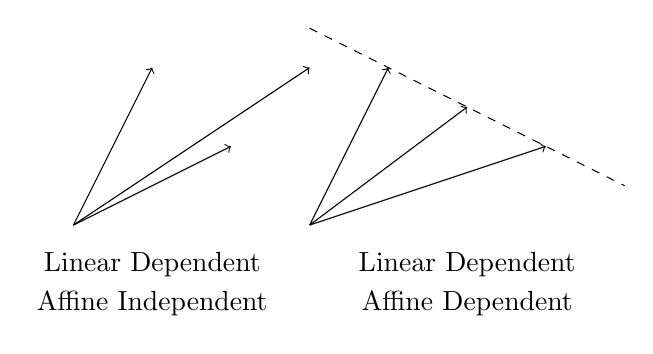
\begin{tikzpicture}
                            \draw [->] (1,1) -- (3,2);
                            \draw [->] (1,1) -- (4,3);
                            \draw [->] (1,1) -- (2,3);
                            \node at (2, 0.5) {Linear Dependent};
                            \node at (2, 0) {Affine Independent};
                            \draw [->] (4,1) -- (5,3);
                            \draw [->] (4,1) -- (6,2.5);
                            \draw [->] (4,1) -- (7,2);
                            \draw [dashed] (4,3.5) -- (8,1.5);
                            \node at (6, 0.5) {Linear Dependent};
                            \node at (6, 0) {Affine Dependent};
                        \end{tikzpicture}
                        \caption{Linearly Independent / Affinely Independent}
                    \end{figure}

                \paragraph{Spanning set and basis}
                    A collection of vectors $v^1, v^2, \dots, v^m$ of dimension $n$ is said to span $\mathcal{R}^n$ if any vector in $\mathcal{R}^n$ can be represented as a linear combination of $v^1, v^2, \dots, v^m$. $v^1, v^2, \dots, v^m$ is said to form a basis of $\mathcal{R}^n$ if the following conditions holds.
                    \begin{itemize}
                        \item $v^1, v^2, \dots, v^m$ span $\mathcal{R}^n$.
                        \item If any of these vectors is deleted, the remaining collection of vector does not span $\mathcal{R}^n$.
                    \end{itemize}

                \paragraph{Rank of a matrix}
                    The span of the columns of a matrix $A$ is called the column space or the range, denoted $range(A)$. The span of the rows of a matrix $A$ is called the row space. The dimension of the column space and row space are equal, which is denoted by $rank(A)$. $rank(A) \le \min\{m,n\}$, if $rank(A) = \min\{m,n\}$, then $A$ is said to have full rank and $A$ is a basis of $\mathcal{R}^n$.

            \subsection{Polyhedral Sets}
                \paragraph{Convex sets}
                    A set $S\subseteq \mathcal{R}^n$ is convex if $\forall x,y \in S, \lambda \in [0,1]$, we have $\lambda x + (1-\lambda)y \in S$

                    \begin{figure}[!htp]
                        \centering
                        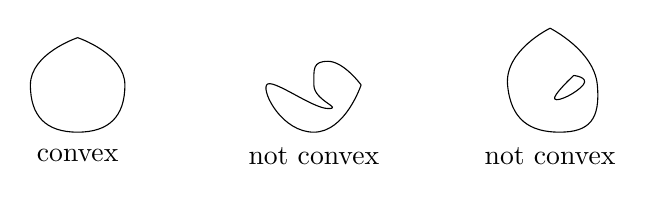
\begin{tikzpicture}[scale=0.6]
                            \draw plot [smooth, tension = 1.2] coordinates{(-5, 1) (-4, 0) (-5, -1) (-6, 0) (-5, 1)};
                            \draw plot [smooth, tension = 1.2] coordinates{(1, 0) (0.3, 0.5) (0, 0) (0.3, -0.5) (-1, 0) (0, -1) (1,0)};
                            \draw plot [smooth, tension = 1.2] coordinates{(5, 1.2) (4.1, 0) (5.2, -1) (6, 0) (5, 1.2)};
                            \draw plot [smooth, tension = 1.2] coordinates{(5.5, 0.2) (5.7, 0) (5.1, -0.3) (5.5, 0.2)};
                            \node at (0,-1.5) {not convex};
                            \node at (-5, -1.5) {convex};
                            \node at (5, -1.5) {not convex};
                        \end{tikzpicture}
                        \caption{A set is convex iff for any two points in the set, the line segment joining those two points lies entirely in the set}
                    \end{figure}

                    Let $x^1, ..., x^k \in \mathcal{R}^n$ and $\lambda \in \mathcal{R}^k$ be given such that $\lambda^Te=1$
                    \begin{itemize}
                        \item The vector $\sum_{i=1}^k \lambda_i x ^i$ is said to be a convex combination of $x^1, ... , x^k$
                        \item The convex hull of $x^1, ... , x^k$ is the set of all convex combinations of these vectors, denoted $conv(x^1, ... ,x^k)$
                    \end{itemize}

                \paragraph{Polyhedral, hyperplanes and half-spaces}
                    \begin{itemize}
                        \item A polyhedron is a set of the form $\{x\in \mathcal{R}^n|Ax\le b\}=\{x \in \mathcal{R}^n | a^ix\le b^i, \forall i \in M\}$, where $A \in \mathcal{R}^{m\times n}$ and $b \in \mathcal{R}^m$
                        \item A polyhedron $P \subset \mathcal{R}^n$ is bounded if there exists a constant $K$ such that $|x_i|<K, \forall x \in P, \forall i \in [1, n]$, in this case the polyhedron is call polytope.
                        \item The lower-bound of $K$ is called diagonal denoted by $d$
                        \item A hyperplane is $\{x\in \mathcal{R}^n|a^Tx=b\}$
                        \item A half-space is $\{x\in \mathcal{R}^n|a^Tx\le b\}$
                    \end{itemize}

                \paragraph{Open, close sets: boundary and interior}
                    \begin{itemize}
                        \item Denote $N_\epsilon = \{y\in \mathcal{R}^n|\lVert y-x\rVert < \epsilon \}$ as the neighborhood of $x\in \mathcal{R}^n$
                        \item Given $S\subseteq \mathcal{R}^n$, x belongs to the interior of $S$, denoted by $int(S)$ if there is $\epsilon > 0$ such that $N_\epsilon(x) \le S$
                        \item $S$ is said to be an open set iff $S=int(S)$
                        \item $x$ belongs to the boundary $\partial S$ if $\forall \epsilon >0$, $N_\epsilon(x)$ contains at least one point in $S$ and a point not in $S$
                        \item $x\in S$ belongs to the closure of $S$, denoted $cl(s)$ if $\forall \epsilon > 0$, $N_\epsilon(x) \cap S = \emptyset$
                        \item $S$ is called closed iff $S=cl(S)$
                        \item In IP, LP, MIP, etc. we always work with close set. No \lq\lq{}$<$\rq\rq{} or \lq\lq{}$>$\rq\rq{}
                    \end{itemize}

                \paragraph{Dimension of polyhedral}
                    \begin{itemize}
                        \item A polyhedron $P$ is dimension $k$, denoted $dim(P)=k$, if the maximum number of affinely independent points in $P$ is $k+1$
                        \item A polyhedron $P\subseteq \mathcal{R}^n$ is full-dimensional if $dim(P) = n$
                        \item Let $M=\{1, 2, ..., m\}$, $M^= = \{i \in M | a_ix=b_i, \forall x \in P\}$, i.e. the equality set, $M^\le = M \setminus  M^=$, i.e. the inequality set. Then, Let $(A^=, b^=)$, $(A^\le, b^\le)$ be the corresponding rows of $(A, b)$, If $P\subseteq \mathcal{R}^n$, then $dim(P) = n - rank(A^=, b^=)$. To proof a constraint $(A^=, b^=)$ is an equality constraint, we need to proof all point in the closure of $P$ satisfied the constraint, to proof it is not an equality constraint, we need to find one point that is not in the hyperplane.
                        \item $x\in P$ is called an inner point of $P$ if $a^ix < b_i, \forall i \in M^\le$
                        \item $x\in P$ is called an interior point of $P$ if $a^ix < b_i, \forall i \in M$
                        \item Every nonempty polyhedron has at least one inner point
                        \item A polyhedron has an interior point iff $P$ is full-dimensional, i.e., there is no equality constraint
                    \end{itemize}

            \subsection{E.P. and B.F.S.}
                \paragraph{Extreme point}
                    A point $x$ in a convex set $X$ is called an extreme point iff $x$ cannot be represented as a strict convex combination of two distinct points of $X$. In other words, if $x = \lambda x_1 + (1 - \lambda) x_2$, then $x_1 = x_2 = x$.

                    An alternative definition is as follows. Let the hyperplanes associated with the $(m + n)$ defining half-spaces of $X$ be referred to as defining hyperplanes of $X$. Furthermore, note that a set of defining hyperplanes are linearly independent if the coefficient matrix associated with this set of equations has full row rank. Then a point $x$ is said to be an extreme point if $x$ lies on some $n$ linearly independent defining hyperplanes of $X$. In addition, if more than $n$ defining hyperplanes pass through an extreme point, then such extreme point is called a degenerated extreme point.

                \paragraph{Basic feasible solution}
                    Consider the system $\{A_{m\times n}x=b_m, x\ge 0\}$, suppose $rank(A, b) = rank(A) =m$, we can arrange $A$ and have a partition of $A$. Let $A=[B, N]$ where $B$ is $m\times m$ invertible matrix, and $N$ is a $m\times (n-m)$ matrix. The solution $x=\left[\begin{matrix}x_B\\x_N\end{matrix}\right]$ to the equation $Ax=b$, where
                    \begin{equation}
                        x_B = B^{-1}b \nonumber
                    \end{equation}
                    and
                    \begin{equation}
                        x_N = 0 \nonumber
                    \end{equation}
                    is called basic solution of system. If $x_B \ge 0$, it is called basic feasible solution. If $x_B > 0$ it is called non-degenerate basic feasible solution. For $x_B \ge 0$, if some $x_j = 0$, those components are called degenerated basic feasible solution. $B$ is called the basic matrix, $N$ is called nonbasic matrix.

                \paragraph{Correspondence between B.F.S and E.P.}
                    \begin{theorem}
                        $x$ is an E.P. iff $x$ is a B.F.S.
                    \end{theorem}
                    
                    \begin{proof}
                        ($\Rightarrow$) If $x$ is an extreme point, by definition, there are (at least) $n$ linearly independent defining hyperplanes at $x$, since $Ax = b$ provides $m$ linearly independent binding hyperplane, there must by some $p = n - m$ additional binding defining hyperplanes from the non-negativity constraints that together with $Ax = b$ provide $n$ linearly independent defining hyperplanes binding at $x$. Denoting these $p$ additional hyperplanes by $x_N = 0$, we therefore conclude that the system $Ax = b, x_N = 0$ has $x$ as the unique solution. Now, let $N$ represent the columns of the variables $x_N$ in $A$, and let $B$ be the remaining columns of $A$ with $x_B$ as the associated variables. Since $Ax = b$ can be written as $Bx_B + Nx_N = b$, this means that $B$ is $m \times m$ and invertible, and moreover, $x_B = B^{-1}b \ge 0$, since $x = (x_B, x_N)$ is a feasible solution. Therefore, $x$ is a basic feasible solution.

                        ($\Leftarrow$) If $x$ is a basic feasible solution, by definition, $x = (x_B, x_N)$ where correspondingly $A = (B, N)$ such that $x_B = B^{-1}b \ge 0$ and $x_N = 0$. This means that the $n$ hyperplanes $Ax = b, x_N = 0$ are binding at $x$ and are linearly independent. Thus, $x$ is an extreme point.
                    \end{proof}

        \section{Simplex Method}
            \subsection{Search Algorithm}
                \paragraph{Improving search algorithm}
                    A simplex method is a search algorithm, for each iteration it finds a not-worse solution, which can be represented as
                    \begin{equation}
                        x^t = x^{t-1}+\lambda_{t-1}d^{t-1} \nonumber 
                    \end{equation}
                    Where $x^t$ is the solution of the $t$th iteration, $\lambda_t$ is the step length of $t$th iteration, and $d^t$ is the direction of the $t$th iteration.
                        
                \paragraph{Optimality test}
                    \begin{align}
                        z &= cx \nonumber\\
                        & = \left[\begin{matrix}c_B & c_N\end{matrix} \right] \left [ \begin{matrix}x_B \\ x_N \end{matrix} \right] \nonumber \\
                        & = c_B x_B + c_N x_N \nonumber \\
                    \text{and } \quad& Ax=b \nonumber \\
                        \Rightarrow & Bx_B + Nx_N = b, x_B\ge 0, x_N\ge 0\nonumber \\
                        \Rightarrow & x_B = B^{-1}b-B^{-1}Nx_N\nonumber \\
                        \Rightarrow & z = c_BB^{-1}b-c_BB^{-1}Nx_N+c_Nx_N\nonumber
                    \end{align}
                    for current solution $\hat{x}=\left [\begin{matrix}\hat{x_B} \\ 0\end{matrix}\right]$, $\hat{z} = c_BB^{-1}b$, then
                    \begin{equation}
                        z - \hat{z} = \left[\begin{matrix}0 & c_N - c_BB^{-1}N \end{matrix} \right] \left[ \begin{matrix}x_B \\ x_N \end{matrix}\right] \nonumber
                    \end{equation}
                    The $c_N - c_BB^{-1}N$ is the reduced cost, for a minimized problem, if $c_N - c_BB^{-1}N > 0$ means $z - \hat{z} \ge 0$, it reaches the optimality because we cannot find a solution less than $\hat{z}$.
                                
                \paragraph{Find direction}
                    Suppose we choose $x_k$ as a candidate to pivot into Basis\\
                    \begin{equation}
                        x = \left[ \begin{matrix}B^{-1}b-B^{-1}a_kx_k \\ 0+e_kx_k\end{matrix}\right]=\left[ \begin{matrix}B^{-1}b \\ 0\end{matrix} \right] + \left[ \begin{matrix} -B^{-1}a_k \\ e_k \end{matrix} \right]x_k \nonumber
                    \end{equation}
                    In this form, we can see: $x$ is the result after $t$th iteration, $\left[ \begin{matrix}B^{-1}b \\ 0\end{matrix} \right]$ is the result after $(t-1)$th iteration. $ \left[ \begin{matrix} -B^{-1}a_k \\ e_k \end{matrix} \right]$ is the iteration direction, $x_k$ is the step length. The only requirement of $x_k$ is $r_k < 0$ where $r_k=c_k - z_k$ is reduce cost, which is the $k$th entry of $c_N - c_BB^{-1}N$. Generally speaking, we usually take $r_k = \min\{c_j - z_j\}$ (which in fact can not guarantee the efficient of the algorithm.)

                \paragraph{Find the step length}
                    We need to guarantee the non-negativity, so for each iteration, we need to make sure $x\ge 0$. Which means
                    \begin{equation}
                        B^{-1}b-B^{-1}a_kx_k \ge 0 \nonumber 
                    \end{equation}
                    Denote $B^{-1}b$ as $\bar{b}$, denote $B^{-1}a_k$ as $y_k$. If $y_k \le 0$, we can have $x_k$ as large as infinite, which means unboundness. If $y_k > 0$ now we can use the minimum ratio to guarantee non-negativity.
                    \begin{equation}
                        \forall i \in B, \bar{b}_i - y_{ik} x_k \ge 0 \Rightarrow x_k = \min_{i \in B} \{\frac{\bar{b}_i}{y_{ik}}, y_{ik} > 0\}.\nonumber
                    \end{equation}

            \subsection{Find Initial Solution}
                \paragraph{Non-trivial case}
                    If some of the constraint is not in $\sum_{i=1}^na_ix_i \le 0$ form, we cannot add a positive slack variable. In this case, we add an artificial variable other than slack variable.
                    \begin{equation}
                        \sum_{i=1}^n a_ix_i \ge (or =) 0 \Rightarrow \sum_{j=1}^n a_ix_i + x_a = 0 \nonumber
                    \end{equation}
                    Notice that in an optimal solution, $x_a = 0$, otherwise it is not valid.\\
                    Artificial variables are only a tool to get the simplex method started. A so-called Two-phase Method is describe in this section.
                
                \paragraph{Two-Phase method}
                    \begin{itemize}
                        \item Phase I: Solve the following program start with a basic feasible solution $x=0, x_a=b$, i.e., the artificial variable forms the basis.
                        \begin{align}
                            \min \quad & 1x_a \nonumber\\
                            \text{s.t.} \quad & Ax + x_a = b \nonumber\\
                                              & x \ge 0 \nonumber\\
                                              & x_a \ge 0 \nonumber
                        \end{align}
                        If the optimal $1x_a \ne 0$, infeasible, stop. Otherwise proceed Phase II.
                        \item Phase II: Remove the columns of artificial variables, replace the objective function with the original objective function, proceed to solve simplex method.
                    \end{itemize}               
                    
                \paragraph{Discussion}
                    \begin{itemize}
                        \item Case A: $x_a \ne 0$. Infeasible.
                        \item Case B.1: $x_a = 0$ and all artificial variables are out of the basis. At the end of Phase I, we derive
                        \begin{align}
                            \begin{tabular} {|c|c|c|c|c|}
                                \hline
                                $x_0$ & $x_B$ & $x_N$ & $x_a$ & RHS \\
                                \hline
                                1 & 0 & 0 & -1 & 0\\
                                \hline
                                0 & $I$ & $B^{-1}N$ & $B^{-1}$ & $B^{-1}b$ \\
                                \hline
                            \end{tabular} \nonumber
                        \end{align}
                        We can discard $x_a$ columns, (or we can leave it because it keeps track of $B^{-1}$), and then we do the Phase II
                        \begin{align}
                            \begin{tabular} {|c|c|c|c|}
                                \hline
                                $z$ & $x_B$ & $x_N$ & $RHS$ \\
                                \hline
                                1 & 0 & $c_BB^{-1}N - c_N$ & $c_BB^{-1}b$ \\
                                \hline
                                0 & $I$ & $B^{-1}N$ & $B^{-1}b$ \\
                                \hline
                            \end{tabular} \nonumber     
                        \end{align}
                        \item Case B.2: Some artificial variables are in the basis at zero values. This is because of degeneracy. We pivot on those artificial variables, once they leave the basis, eliminate them.
                    \end{itemize}

            \subsection{Degeneracy and Cycling}
                \paragraph{Degeneracy}
                    If the basic variable $x_B$ is not strictly $> 0$, i.e. if some basic variable equals to 0, we call it degenerate.

                \paragraph{Cycling}
                    In the degenerate case, pivoting by the simplex rule does not always give a strict decrease in the objective function value, because it may have $b_r = 0$. It is possible that the tableau may repeat if we use the simplex rule.Geometrically speaking, it means that at the same point - extreme point - it corresponds to more than one feasible solutions, so when we are pivoting, we stays at the same place. However, in computer algorithm, we rarely care about cycling because the data in computer is not precise, it is very hard to get into cycling.

                \paragraph{Cycling prevent}
                    \begin{itemize}
                        \item Lexicographic rule
                        \begin{itemize}
                            \item For entering variable, same as simplex rule
                            \item For leaving variable, if there is a tie, choose the variable with the smallest $\frac{y_{r1}}{y_{rk}}$.
                        \end{itemize}
                        \item Bland's rule
                        \begin{itemize}
                            \item For entering variable, choose the variable with smallest index where $z_j - c_j \le 0$
                            \item For leaving variable, if there is a tie, choose the variable with smallest index.
                        \end{itemize}
                        \item Successive ratio rule
                        \begin{itemize}
                            \item Select the pivot column as any column $k$ where $z_k - c_k \le 0$
                            \item Given $k$, select the pivot row $r$ as the minimum successive ratio row associated with column $k$. In other words, for pivot columns where there is no tie in the usual minimum ratio, the successive ratio rule reduces to the simplex rule.
                        \end{itemize}
                    \end{itemize}

        \section{Revised Simplex Method}
            \subsection{Key to Revised Simplex Method}
                The procedure of Simplex Method is (almost) exactly the same as original simplex method. However, notice that we don't need to use $N$ so for the revised simplex method, we don't calculate any matrix related to $N$

                The original matrix:

                \begin{align}
                    \begin{tabular} {|c|c|c|c|}
                        \hline
                        $z$ & $x_B$ & $x_N$ & $RHS$ \\
                        \hline
                        1 & 0 & $c_BB^{-1}N - c_N$ & $c_BB^{-1}b$ \\
                        \hline
                        0 & $I$ & $B^{-1}N$ & $B^{-1}b$ \\
                        \hline
                    \end{tabular} \nonumber     
                \end{align}

                The revised matrix:

                \begin{align}
                    \begin{tabular} {|c|c|}
                        \hline
                        Basic Inverse & RHS \\
                        \hline
                        $w=c_BB^{-1}$ & $c_B\bar{b} = c_BB^{-1}b$\\
                        \hline
                        $B^{-1}$ & $\bar{b} = B^{-1}b$\\
                        \hline
                    \end{tabular} \nonumber
                \end{align}

                For each pivot iteration, calculate $z_j - c_j = wa_j - c_j = c_BB^{-1}a_j - c_j, \forall j\in N$, pivot rules are the same as simplex method, each time find a variable $x_k$ to enter basis

                \begin{align}
                    \begin{tabular}{|c|c|c|c|}
                        \cline{1-2} \cline{4-4} $B^{-1}$ & RHS & & $x_k$ \\
                        \cline{1-2} \cline{4-4} $w$ & $c_B\bar{b}$ & & $z_k-c_k$ \\
                        \cline{1-2} \cline{4-4} $B^{-1}$ & $\bar{b}$ & & $y_k$ \\
                        \cline{1-2} \cline{4-4}
                    \end{tabular} \nonumber
                \end{align}

                Do the minimum ratio rule to find the variable $x_r$ to leave the basis

                \begin{align}
                    \begin{tabular}{|c|c|c|c|}  
                        \cline{1-2} \cline{4-4} $B^{-1}$ & RHS & & $x_k$ \\
                        \cline{1-2} \cline{4-4} $w$ & $c_B\bar{b}$ & & $z_k-c_k$ \\
                        \cline{1-2} \cline{4-4} & $\bar{b}_1$ & & $y_{1k}$\\
                        & $\bar{b_2}$ & & $y_{2k}$\\
                        & $\cdots$ & & $\cdots$\\
                        $B^{-1}$ & $\bar{b}_r$ & & $y_{rk}$(pivot at here)\\
                        & $\cdots$ & & $\cdots$\\
                        & $\bar{b}_m$ & & $y_{mk}$\\
                        \cline{1-2} \cline{4-4} 
                    \end{tabular} \nonumber
                \end{align}

            \subsection{Comparison between Simplex and Revised Simplex}
                \paragraph{Advantage of revised simplex}
                    \begin{itemize}
                        \item Save storage memory
                        \item Don\rq{}t need to calculate N (including $B^{-1}N$ and $c_BB^{-1}N$)
                        \item More accurate because round up errors will not be accumulated 
                    \end{itemize}

                \paragraph{Disadvantage of revised simplex}
                    Need to calculate $wa_j$ for all $j \in N$ (in fact don\rq{}t need to calculated it for the variable just left the basis) 

                \paragraph{Computation complexity}
                    \begin{align}
                        \begin{tabular}{|c|c|c|}
                            \hline Method & Type & Operations\\
                            \hline Simplex & $\times$ & $(m+1)(n-m+1)$\\
                            \cline{2-3} & $+$ & $m(n-m+1)$\\
                            \hline Revised Simplex & $\times$ & $(m+1)^2+m(n-m)$ \\
                            \cline{2-3} & $+$ & $m(m+1)+m(n-m)$ \\
                            \hline
                        \end{tabular} \nonumber
                    \end{align}

                \paragraph{When to use?}
                    \begin{itemize}
                        \item When $m >> n$, do revise simplex method on the dual problem
                        \item When $m \simeq n$, revise simplex method is not as good as simplex method
                        \item When $m << n$ perfect for revise simplex method.
                    \end{itemize}
                            
            \subsection{Decomposition of B inverse}
                Let $B=\{ a_{B_1}, a_{B_2}, ..., a_{B_r}, ..., a_{B_m}\}$ and $B^{-1}$ is known.
                If $a_{B_r}$ is replaced by $a_{B_k}$, then $B$ becomes $\bar{B}$. Which means $a_{B_r}$ enters the basis and $a_{B_k}$ leaves the basis. \\
                Then $\bar{B}^{-1}$ can be represent by $B^{-1}$. Noting that $a_k=By_k$ and $a_{B_i}=Be_i$, then
                \begin{align}
                    \bar{B} & = (a_{B_1}, a_{B_2}, ...,a_{B_{r-1}}, a_k, a_{B_{r+1}}, a_m) \nonumber \\
                    & = (Be_1, Be_2, ..., Be_{r-1}, By_k, Be_{r+1}, ..., Be_m) \nonumber \\
                    & = BT \nonumber
                \end{align}
                where $T$ is
                \begin{equation}
                    T=\left[ \begin{array}{cccccccc}
                        1 & 0 & ... & 0 & y_{1k} & 0 & ... & 0 \\
                        0 & 1 & ... & 0 &  y_{2k} & 0 & ... & 0 \\
                        \vdots & \vdots & & \vdots & \vdots & \vdots & & \vdots \\
                        0 & 0 & ... & 1 & y_{r-1,k} & 0 & ... & 0 \\
                        0 & 0 & ... & 0 & y_{rk} & 0 & ... & 0 \\
                        0 & 0 & ... & 0 &  y_{r+1,k} & 1 & ... & 0 \\
                        \vdots & \vdots & & \vdots & \vdots & \vdots & & \vdots \\
                        0 & 0 & ... & 0 &  y_{mk}& 0 & ... & 1 \\
                    \end{array} \right] \nonumber
                \end{equation}
                and 
                \begin{equation}
                    E =  T ^{-1}=\left[ \begin{array}{cccccccc}
                        1 & 0 & ... & 0 & \frac{-y_{1k}}{y_{rk}} & 0 & ... & 0 \\
                        0 & 1 & ... & 0 & \frac{-y_{2k}}{y_{rk}} & 0 & ... & 0 \\
                        \vdots & \vdots & & \vdots & \vdots & \vdots & & \vdots \\
                        0 & 0 & ... & 1 & \frac{-y_{r-1,k}}{y_{rk}} & 0 & ... & 0 \\
                        0 & 0 & ... & 0 & \frac{1}{y_{rk}} & 0 & ... & 0 \\
                        0 & 0 & ... & 0 & \frac{-y_{r+1,k}}{y_{rk}} & 1 & ... & 0 \\
                        \vdots & \vdots & & \vdots & \vdots & \vdots & & \vdots \\
                        0 & 0 & ... & 0 &  \frac{-y_{mk}}{y_{rk}} & 0 & ... & 1 \\
                    \end{array} \right] \nonumber
                \end{equation}
                For each iteration, i.e. one variable enters the basis and one leaves the basis, $\bar{B}^{-1}=T^{-1}B^{-1}=EB^{-1}$. Given that the first iteration starts from slack variables, the first basis $B_1$ is $I$, then we have
                \begin{equation}
                    B^{-1}_t=E_{t-1} E_{t-2} \cdots E_{2} E_{1} I\nonumber
                \end{equation}
                Using $E$ in calculation can simplify the product of matrix where
                \begin{align}
                    cE &= {c_1,c_2,...,c_m} \left[ \begin{array}{cccccc}
                    1 & 0 & ... & g_1 & ... & 0 \\
                    0 & 1 & ... & g_2 & ... & 0 \\
                    \vdots & \vdots & & \vdots & & \vdots \\
                    0 & 0 & ... & g_m & ... & 1 \\
                    \end{array} \right] \nonumber \\
                    &= (c_1, c_2, ... ,c_{r-1}, cg, c_{r+1}, ..., c_m) \nonumber
                \end{align}
                and
                \begin{align}
                    Ea &=  \left[ \begin{array}{cccccc}
                    1 & 0 & ... & g_1 & ... & 0 \\
                    0 & 1 & ... & g_2 & ... & 0 \\
                    \vdots & \vdots & & \vdots & & \vdots \\
                    0 & 0 & ... & g_m & ... & 1 \\
                    \end{array} \right]
                     \left[ \begin{array}{c}
                    a_1 \\
                    a_2 \\
                    \vdots \\
                    a_m \\
                    \end{array} \right] \nonumber \\
                    &= 
                    \left[ \begin{array}{c}
                    a_1 \\
                    a_2 \\
                    \vdots \\
                    a_{r-1} \\
                    0 \\
                    a_{r+1} \\
                    \vdots \\
                    a_m \\
                    \end{array} \right] +
                    a_r\left[ \begin{array}{c}
                    g_1 \\
                    g_2 \\
                    \vdots \\
                    g_{r-1} \\
                    g_r \\
                    g_{r+1} \\
                    \vdots \\
                    g_m \\
                    \end{array} \right] \nonumber \\
                    &=\bar{a}+a_rg \nonumber
                \end{align}
                Then we can calculate $w$, $y_k$ and $\bar{b}$
                \begin{align}
                    w&=c_BB^{-1} = c_BE_{t-1}E_{t-2}...E_2E_1 \nonumber \\
                    y_k &=B^{-1}a_k = E_{t-1}E_{t-2}...E_2E_1a_k \nonumber \\
                    \bar{b}&=B^{-1}_{t+1}b=E_tE_{t-1}E_{t-2}...E_2E_1b \nonumber
                \end{align}

        \section{Duality}
            \subsection{Dual Formulation}
                For any prime problem
                \begin{align}
                    \text{min} \quad & cx \nonumber\\
                    \text{s.t.} \quad & Ax\ge b \nonumber\\
                                & x\ge 0 \nonumber
                \end{align}
                we can have a dual problem
                \begin{align}
                    \text{max} \quad & wb \nonumber \\
                    \text{s.t.} \quad & wA\le c\nonumber\\
                                & w \ge 0\nonumber
                \end{align}
                
            \subsection{Mixed Forms of Duality}
                For the following prime problem
                \begin{align}
                    \text{P(or D)} \quad \min \quad & c_1x_1 + c_2x_2 + c_3x_3 \nonumber\\
                    \quad \text{s.t.} \quad & A_{11}x_1 + A_{12}x_2 + A_{13}x_3 \ge b_1 \nonumber\\
                                            & A_{21}x_1 + A_{22}x_2 + A_{23}x_3 \le b_2 \nonumber\\
                                            & A_{31}x_1 + A_{32}x_2 + A_{33}x_3 = b_3 \nonumber\\
                                            & x_1 \ge 0 \nonumber\\
                                            & x_2 \le 0 \nonumber\\
                                            & x_3 \quad \text{unrestricted} \nonumber
                \end{align}
                The dual of the problem
                \begin{align}
                    \text{D(or P)} \quad \max \quad & w_1b_1 + w_2b_2 + w_3b——3 \nonumber\\
                    \quad \text{s.t.} \quad & w_1A_{11} + w_2A_{21} + w_3A_{31} \le c_1 \nonumber\\
                                            & w_1A_{12} + w_2A_{22} + w_3A_{32} \ge c_2 \nonumber\\
                                            & w_1A_{13} + w_2A_{23} + w_3A_{33} = c_3 \nonumber\\
                                            & w_1 \ge 0 \nonumber\\
                                            & w_2 \le 0 \nonumber\\
                                            & w_3 \quad \text{unrestricted} \nonumber
                \end{align}
                In sum, the relation between primal and dual problems are listed as following\\
                \begin{table}[!htp]
                    \centering
                    \begin{tabular}{|c|c|c|c|c|}
                        \hline & Minimization& & Maximization& \\
                        \hline & $\geq 0$ & $\longleftrightarrow$ & $\leq 0$ & \\
                        Var & $\leq 0$ & $\longleftrightarrow$ & $\geq 0$ & Cons \\
                        & Unrestricted & $\longleftrightarrow$ & = & \\
                        \hline & $\geq 0$ & $\longleftrightarrow$ & $\geq 0$ & \\
                        Cons & $\leq 0$ & $\longleftrightarrow$ & $\leq 0$ & Var \\
                        & = & $\longleftrightarrow$ & Unrestricted & \\
                        \hline
                    \end{tabular}
                \end{table}                

            \subsection{Primal-Dual Relationships}
                \paragraph{Weak duality property}
                    Let $x_0$ be any feasible solution of a primal minimization problem,
                    \begin{equation}
                        Ax_0 \ge b, \quad x_0\ge 0 \nonumber
                    \end{equation}
                    Let $x_0$ be any feasible solution of a dual maximization problem,
                    \begin{equation}
                        w_0A \le c, \quad w_0\ge 0 \nonumber
                    \end{equation}
                    Therefore, we have
                    \begin{equation}
                        cx_0 \ge w_0Ax_0 \ge w_0b \nonumber
                    \end{equation}
                    which is called the weak duality property. This property is for any feasible solution in the primal and dual problem.\\
                    Therefore, any feasible solution in the maximization problem gives the lower bound of its dual problem, which is a minimization problem, vice versa. We use this to give the bounds in using linear relaxation to solve IP problem.

                \paragraph{Fundamental theorem of duality}
                    With regard to the primal and dual LP problems, one and only one of the following can be true. 

                    \begin{itemize}
                        \item Both primal and dual has optimal solution $x^*$ and $w^*$, where $cx^* = w^*b$
                        \item One problem has an unbounded optimal objective value, the other problem must be infeasible
                        \item Both problems are infeasible.
                    \end{itemize}

                    \begin{table}[!htp]
                        \centering
                        \begin{tabular}{|c|c|c|}
                            \hline P & & D \\
                            \hline Optimal & $\Rightarrow$ & Optimal \\
                            Degeneracy & & Multiple optimal \\
                            (or Multiple optimal) & & (or Degeneracy) \\
                            \hline Infeasible & $\Rightarrow$ & Unbounded or Infeasible \\
                            \hline Unbounded & $\Rightarrow$ & Infeasible \\
                            \hline
                        \end{tabular}
                    \end{table}

                \paragraph{Strong duality property}
                    From KKT condition, we know that in order to make $x^*$ the optimal solution, the following condition should be met.
                    \begin{itemize}
                        \item Primal Optimal: $Ax^* \ge b$, $x^*\ge 0$
                        \item Dual Optimal: $w^*A \le c$, $w^*\ge 0$
                        \item Complementary Slackness:
                    \begin{equation}
                        \begin{cases}
                            w^*(Ax^*-b) = 0\\
                            (c-w^*A)x^* = 0
                        \end{cases} \nonumber
                    \end{equation}
                    \end{itemize}
                    The first condition means the primal has an optimal solution, the second condition means the dual has an optimal solution. The third condition means $cx^*=w^*b$, which is also called strong duality property.

                \paragraph{Complementary slackness theorem}
                    Let $\bm{x^*}$ and $\bm{w^*}$ be any feasible solutions, they are optimal iff
                    \begin{align}
                        (c_j - \bm{w^*}\bm{a_j})x_j^* &= 0, \quad j = 1,...,n\nonumber \\
                        w_i^*(\bm{a^i}\bm{x^*} - b_i) &= 0, \quad i = 1,...,m\nonumber
                    \end{align}
                    In particular
                    \begin{align}
                        x_j^*>0 &\Rightarrow \bm{w^*}\bm{a_j} = c_j \nonumber \\
                        \bm{w^*}\bm{a_j} < c_j &\Rightarrow x_j^* = 0 \nonumber \\
                        w_i^* >0 &\Rightarrow \bm{a^i}\bm{x^*} = b_i \nonumber \\
                        \bm{a^i}\bm{x^*} > b_i &\Rightarrow w_i^*=0\nonumber
                    \end{align}
                    It means, if in optimal solution a variable is positive (has to be in the basis), the correspond constraint in the other problem is tight. If the constraint in one problem is not tight, the correspond variable in the other problem is zero.

                \paragraph{Use dual to solve the primal}
                    in the dual problem, we solved some $w$ which is positive, we can know that the correspond constraint in primal is tight, furthermore we can solve the basic variables from those tight constraints, which becomes equality and we can solve it using Gaussian-Elimination.

            \subsection{Shadow Price}
                \paragraph{Shadow price under non-degeneracy}
                    Let $B$ be an optimal basis for primal problem and the optimal solution $x^*$ is non-degenerated.
                    \begin{equation}
                        z=c_BB^{-1}b - \sum_{j\in N}(z_j - c_j)x_j = w^*b - \sum_{j\in N}(z_j - c_j)x_j \nonumber
                    \end{equation}
                    therefore
                    \begin{equation}
                        \frac{\partial z^*}{\partial b_i} = c_BB^{-1}_i = w_i^* \nonumber
                    \end{equation}
                    $w^*$ is the shadow prices for the right-hand-side vectors. We can also regard it as the incremental cost of producing one more unit of the $i$th product. Or $w^*$ is the fair price we would pay to have an extra unit of the $i$th product.

                \paragraph{Shadow price under degeneracy}
                    For shadow price under degeneracy, the $w^*$ may not be the true shadow price, for it may not be the right basis. In this case, the partial differentiation may not be valid, for component $b_i$, if $x_i = 0$ and $x_i$ is a basic variable, we can't find the differentiation.

            \subsection{Dual Simplex Method}
                Occasionally, an initial feasible solution for the Simplex Method might be difficult to acquired, for example, when $\mathbf{0}$ is not an initial solution, or, in some other cases, a basic infeasible solution is known in advance. To solve the LP, we can take advantage of the LP Strong Duality Theorem, and solve the dual problem to optimality instead of the prime problem. Such technique is called the Dual Simplex Method. The details of such method is as follows (for minimization problems)

                \begin{enumerate}
                    \item Choose an initial basic solution $x_B$ and corresponding basis matrix $B$ so that $c_BB^{-1}A_j - c_j \ge 0$ for all $j \in J$, where $J$ is the set of non-basic variables.
                    \item Construct a simplex tableau using this initial solution.
                    \item If $\bar{b} = B^{-1}b \ge 0$, then an optimal solution has been achieved; STOP. Otherwise, the dual problem is feasible, GOTO STEP 4.
                    \item Choose a leaving variable $x_{B_i} = \bar{b}_i$ so that $\bar{b}_i < 0$
                    \item Choose the index of the entering variable $x_j$ using the following minimum ratio test:
                    \begin{equation*}
                        \frac{z_j - c_j}{\bar{a}_{j_i}} = \min \{\frac{z_k - c_k}{\bar{a}_{k_i}}|k \in J, \bar{a}_{j_i} < 0\}
                    \end{equation*}
                    \item If no entering variable can be selected ($\bar{a}_{j_i} \ge 0, \forall k \in K$) then the dual problem is unbounded and the prime problem is infeasible. STOP
                    \item Using a standard simplex pivot, on element $\bar{a}_{j_i}$, thus causing $w_{B_i}$ to become 0 (and thus feasible) and causing $x_j$ to enter the basis. GOTO STEP 3.
                \end{enumerate}

                In general, the Dual Simplex Method is (almost) the same as a Simplex Method. The Dual Simplex Method starts with an infeasible basic solution, during each iteration, it maintains dual feasibility and work towards primal feasibility. In Dual Simplex Method, the old Right Hand Side becomes new $z_j - c_j$, and the old $z_j - c_j$ become new Right Hand Side.

    \chapter{Computational Complexity} 
        \begin{center}
            \texttt{``import numpy as np''}
        \end{center}

        \section{Preliminaries}
            \subsection{How difficult is to solve an integer program?}
                \begin{itemize}
                    \item Hard!
                    \item What is ``hard''? $\Rightarrow$ measurement of difficulties.
                    \item $\Rightarrow$ computational complexity $\Rightarrow$ the art of classifying computational problems according to their resource usage.
                    \item What is ``algorithm''? $\Rightarrow$ Given a string $s$, an algorithm takes the input $s$ and within finite number of steps, returns an output string $s^\prime$.
                    \item What is ``resource usage''? $\Rightarrow$ How much \textit{time}/\textit{space} it takes for an algorithm to process $s$?
                \end{itemize}

            \subsection{Asymptotic Notation}
                \paragraph{$O$-Notation}
                    Let $f(n)$ and $g(n)$ be real functions. We say $f(n) = O(g(n))$ if there exist positive constants $n_0$ and $c$ such that
                    \begin{equation*}
                        0 \le f(n) \le cg(n), \quad \forall n \ge n_0
                    \end{equation*}

                    A common trick that finds $O(g(n))$ for $f(n)$ is to find function $g(n)$ such that 
                    \begin{equation*}
                        \lim_{n \rightarrow \infty} \frac{f(n)}{g(n)} = C \quad \text{(constant)}
                    \end{equation*}

                    The $O$-Notation is referred as the asymptotic upper bound. The $O$-Notation is more widely used, since it can provide a clear estimate of the worst case time/space complexity of an algorithm that exclusively considers the critical grow factors.

                \paragraph{$\Omega$-Notation}
                    Let $f(n)$ and $g(n)$ be real functions. We say $f(n) = \Omega(g(n))$ if there exist positive constants $n_0$ and $c$ such that
                    \begin{equation*}
                        0 \le cg(n) \le f(n), \quad \forall n \ge n_0
                    \end{equation*}

                    The $\Omega$-Notation is referred as the asymptotic lower bound. In addition:

                    \begin{theorem}
                        $f(n) = O(g(n)) \Leftrightarrow g(n) = \Theta(f(n))$
                    \end{theorem}
                
                \paragraph{$\Theta$-Notation}
                    Let $f(n)$ and $g(n)$ be real functions. We say $f(n) = \Theta(g(n))$ if there exist positive constants $n_0$, $c_1$, and $c_2$ such that
                    \begin{equation*}
                        c_1g(n) \le f(n) \le c_2g(n), \quad \forall n \ge n_0
                    \end{equation*}

                    The $\Theta$-Notation is referred as the asymptotic tight bound. In addition:

                    \begin{theorem}
                        $f(n) = \Theta(g(n)) \Leftrightarrow f(n) = O(g(n)) \text{ and } f(n) = \Omega(g(n))$
                    \end{theorem}

        \section{P v.s. NP}
            \subsection{P and NP}
                \paragraph{Decision problem} A decision problem $X$ is the set of strings on which the output is yes, i.e., $s \in X$ iff the correct output for the input $s$ is 1 (yes).

                    \begin{example}
                        The optimization version of the knapsack problem: Given a set of items $N$, each item $i \in N$ having a weight $w_i$ and a value $c_i$, a capacity $b$ and a threshold value $k$, find a collection of items $S \subseteq N$ of the maximum value whose total weight is less than or equal to $b$. The output is a set $S$.

                        The decision version of the knapsack problem: Given a set of items $N$, each item $i \in N$ having a weight $w_i$ and a value $c_i$, a capacity $b$ and a threshold value $k$, determine if there exists a collection of items $S \subseteq N$ whose total weight is less than or equal to $b$ and its total value is at least $k$. The output is a boolean value, True/False.
                    \end{example}

                    If we have an algorithm to solve the optimization version of knapsack problem, we can immediately solve the decision version. 

                \paragraph{Class $P$}
                    \begin{definition}[polynomial running time]
                        Algorithm $A$ has polynomial running time if there is a polynomial function $p(\dot)$ such that for every string $s$, $A$ terminates on $s$ in at most $p(|s|)$ steps.
                    \end{definition}

                    \begin{definition}[Class $P$]
                        The complexity class $P$ is the set of decision problems $X$ that can be solved in polynomial time.
                    \end{definition}

                    That is, there is a known algorithm that provides the solution of any instance of size $n$ in time $n^{O(1)}$.

                    \begin{example} The following problems are known as in class $P$:
                        \begin{itemize}
                            \item Shortest path problem
                            \item Maximum flow problem
                            \item Spanning tree problem
                            \item Linear programming (but not the simplex method)
                            \item Assignment problem
                        \end{itemize}
                    \end{example}

                \paragraph{Class NP}
                    \begin{definition}[certifier, certificate]
                        $B$ is an efficient certifier for a problem $X$ if
                        \begin{itemize}
                            \item $B$ is a polynomial-time algorithm that takes two input strings $s$ and $t$
                            \item There is a polynomial function $p$ such that $s \in X$ if and only if there is a string $t$ such that $|t| \le p(|s|)$ and $B(s, t) = 1$
                        \end{itemize}
                        The string $t$ such that $B(s, t) = 1$ is called a certificate.
                    \end{definition}

                    \begin{example}
                        Q: Given a graph $G = (V, E)$ with a Hamiltonian cycle, how can one convince another there exists a Hamiltonian cycle? 

                        A: One can send a string (certificate) to another, the other will run an algorithm (certifier) to check if the string represents a Hamiltonian cycle.
                    \end{example}

                    \begin{definition}[class NP]
                        The complexity class NP is the set of all problems for which there exists an polynomial-time certifier.
                    \end{definition}

                \paragraph{P v.s. NP}
                    \begin{itemize}
                        \item Is $P = NP?$ This is the most famous and fundamental open problem in computer science.
                        \item Most people believe $P \neq NP$.
                        \item If $P = NP$, that means if one can check a solution in polynomial time, one can solve it in polynomial time.
                        \item We are sure that $P \subseteq NP$
                    \end{itemize}

            \subsection{Polynomial Time Reduction}
                \paragraph{Polynomial-time reducible} Given a black box algorithm $A$ that solves a problem $X$, if any instance of a problem $Y$ can be solved using a polynomial number of standard computational steps, plus a polynomial number of calls to $A$, then we say $Y$ is polynomial-time reducible to $X$, denoted as $Y \le_P X$.

                Suppose $Y \le_P X$:
                \begin{itemize}
                    \item If $X$ can be solved in polynomial time, then $Y$ can be solved in polynomial time.
                    \item If $Y$ cannot be solved in polynomial time, then $X$ cannot be solved in polynomial time.
                \end{itemize}

                $X$ is at least as hard as $Y$.

            \subsection{NP-Completeness}
                \paragraph{NP-Completeness}
                    A problem $X$ is called NP-complete if
                    \begin{itemize}
                        \item $X \in NP$, and
                        \item $Y \le_P X$, for every $Y \in NP$
                    \end{itemize}

                    If any NP-complete problem can be solved in polynomial time, then $P = NP$. Unless $P = NP$, a NP-complete problem cannot be solved in polynomial time.

                \paragraph{Circuit-Sat}
                    The Circuit Satisfiability problem is the first NP-complete problem.

                    \begin{theorem}[Cook's Theorem]
                        SAT is NP-Complete
                    \end{theorem}

                    \begin{figure}[H]
                        \centering
                        \includegraphics[width=0.5\textwidth]{../../image/circuit.png}
                    \end{figure}

                    \begin{itemize}
                        \item key fact: any algorithm that takes $n$ bits as input and outputs $0/1$ with running time $T(n)$ can be converted into a circuit of size $p(T(n))$ for some polynomial function $p(\cdot)$.
                        \item Then, we can show that any problem $Y \in NP$ can be reduced to Circuit-Sat
                    \end{itemize}

                \paragraph{Reductions of NP-Complete problems}
                    We will show a SAT $\le_P$ 3-SAT

                    \begin{definition}[3-CNF]
                        3-CNF is a special case of formula:
                        \begin{itemize}
                            \item Boolean variables: $x_1, x_2, \cdots, x_n$
                            \item Literals: $x_i$ or $\bar{x_i}$
                            \item Clause: disjunction (``or'') of at most 3 literals
                            \item 3-CNF formula: conjunctino (``and'') of clauses.
                        \end{itemize}
                    \end{definition}

                    \begin{example}
                        This is a 3-CNF: $(x_1 \vee x_2 \vee x_3) \wedge (x_2 \vee \bar{x_3} \vee x_4)$
                    \end{example}

                    To satisfy a 3-CNF, we need to satisfy all clauses. To satisfy a clause, we need to satisfy at least 1 literal. Associate every wire with a new variable, the circuit will be equivalent to a formula. Each formula can be transformed into a 3-CNF. 

                    The SAT is satisfiable iff the 3-CNF is satifiable, and the size of the 3-CNF formula is polynomial in the size of the circuit. Thus SAT $\le_P$ 3-SAT.

                    For other problems, here is a polynomial-reducible relation graph for reference.

                    \begin{figure}[H]
                        \centering
                        \includegraphics[width=0.8\textwidth]{../../image/polyRedu.png}
                    \end{figure}

        \section{Algorithm Analysis and Design}
            \subsection{Three programming paradigms}
                \paragraph{Greedy Algorithm}
                    \begin{itemize}
                        \item Make a greedy choice
                        \item At each step, make an irrevocable decision using a ``reasonable'' strategy
                        \item Prove that the greedy choice is safe
                        \item Show that the remaining task after applying the strategy is to solve a/many \textbf{smaller instance}(s) of the same problem
                        \item Usually for optimization problems.
                    \end{itemize}

                \paragraph{Dynamic Programming}
                    \begin{itemize}
                        \item Break up a problem into many \textbf{overlapping} sub-problems
                        \item Build solutions for larger and larger sub-problems
                        \item Use a table/dictionary to store solutions for sub-problems for reuse
                    \end{itemize}

                \paragraph{Divide and Concur}
                    \begin{itemize}
                        \item Break a problem into many \textbf{independent} sub-problems
                        \item Solve each sub-problem separately
                        \item Combine solutions for sub-problems to form a solution for the original one
                        \item Usually used to design more efficient algorithms
                    \end{itemize}

            \subsection{Master Theorem}
                \begin{theorem}
                    $T(n) = aT(n/b) + O(n^c)$, where $a \ge 1, b > 1, c \ge 0$ are constants. Then,
                    \begin{equation*}
                        T(n) = \begin{cases}
                            & O(n^{\log_b a}) \quad \text{if } c < \log_b a\\
                            & O(n^c \log n) \quad \text{if } c = \log_b a\\
                            & O(n^c) \quad \text{if } c > \log_b a
                        \end{cases}
                    \end{equation*}
                \end{theorem}

                \begin{figure}[H]
                    \centering
                    \includegraphics[width=0.8\textwidth]{../../image/masterTheorem.png}
                    \label{fig:masterTheorem}
                \end{figure}

                \begin{itemize}
                    \item $c < \log_b a$: bottom-level dominates, $(\frac{a}{b^c})^{\log_b n} n^c = O(n^{\log_b a})$
                    \item $c = \log_b a$: all levels have same time, $n^c \log_b n = O(n^c \log n)$
                    \item $c > \log_b a$: top-level dominates, $O(n^c)$
                \end{itemize}

        \section{Some examples}
            \subsection{Minimum Spanning Tree Problem}
                \paragraph{Basic Concepts}
                    \begin{example}
                        A company wants to build a communication network for their offices. For a link between office $v$ and office $w$, there is a cost $c_{vw}$. If an office is connected to another office, then they are connected to with all its neighbors. Company wants to minimize the cost of communication networks.
                    \end{example}

                    \begin{definition}[Minimum spanning tree problem]
                        Given a connected graph graph $G$, and a cost $C_e, \forall e\in E$, find a minimum cost spanning tree of $G$
                    \end{definition}

                \paragraph{Kruskal's Algorithm}
                    Let's start with a greedy algorithm

                    \begin{algorithm}[H]
                        \caption{MST-Greedy(G, w)}
                        \begin{algorithmic}[1]
                            \State $F = \emptyset$
                            \State Sort edges in $E$ in non-decreasing order of weight $w$
                            \For {$e = (u, v)$}
                                \If {$u$ and $v$ are not connected by a path of edge in $F$}
                                    \State $F = F \cup \{(u, v)\}$
                                \EndIf
                            \EndFor
                            \State \Return $F$
                        \end{algorithmic}
                    \end{algorithm}


                    The Kruskal's algorithm is as follows
                    \begin{algorithm}[H]
                        \caption{Kruskal's Algorithm}
                        \begin{algorithmic}
                            \State $F \gets \emptyset$
                            \State $S \gets \{\{v\}: v \in V\}$
                            \State Sort edges in $E$ in non-decreasing order of weight $w$
                            \For {$e = (u, v)$}
                                \State $S_u \gets$ the set in $S$ containing $u$
                                \State $S_v \gets$ the set in $S$ containing $v$
                                \If {$S_u \neq S_v$}
                                    \State $F \gets F \cup \{(u, v)\}$
                                    \State $S \gets S \setminus \{S_u\} \setminus \{S_v\} \cup \{S_u \cup S_v\}$
                                \EndIf
                            \EndFor
                            \State \Return $F$
                        \end{algorithmic}
                    \end{algorithm}

                \paragraph{Prim's Algorithm}
                    Let's start with another greedy algorithm
                    \begin{algorithm}[H]
                        \caption{MST-Greedy(G, w)}
                        \begin{algorithmic}
                            \State $S \gets \{s\}$, where $s$ is arbitary vertex in $V$
                            \State $F \gets \emptyset$
                            \While {$S \neq V$}
                                \State $(u, v) \gets$ the lightest edge between $S$ and $V \setminus S$, where $u \in S$ and $v \in V \setminus S$
                                \State $S \gets S \cup \{v\}$
                                \State $F \gets F \cup \{(u, v)\}$
                            \EndWhile
                        \end{algorithmic}
                    \end{algorithm}

                    The Prim's algorithm is as follows
                    \begin{algorithm}[H]
                        \caption{Prim's Algorithm}
                        \begin{algorithmic}
                            \State $s \gets$ arbitary vertex in $G$
                            \State $S \gets \emptyset$, $d(s) \gets 0$ and $d(v) \gets \infty$ for every $v \in V \setminus \{s\}$
                            \While {$S \neq V$}
                                \State $u \gets $ vertex in $V\setminus S$ with minimum $d(u)$
                                \State $S \gets S \cup \{u\}$
                                \For {Each $v \in V \setminus S$ such that $(u, v) \in E$}
                                    \If {$w(u, v) < d(v)$}
                                        \State $d(v) \gets w(u, v)$
                                        \State $\pi(v) \gets u$
                                    \EndIf
                                \EndFor
                            \EndWhile
                            \State \Return $\{(u, \pi(u))| u \in V \setminus \{s\}\}$
                        \end{algorithmic}
                    \end{algorithm}

            \subsection{Knapsack Problem}
                \paragraph{Integer program model}
                    \begin{align}
                        \max \quad & \sum_{i \in S} v_i\\
                        \text{s.t.} \quad & \sum_{i \in S} w_i \le W\\
                        & w_i \ge 0, \forall i \in S
                    \end{align}

                \paragraph{Solve knapsack problem by dynamic programming}
                    \begin{itemize}
                        \item Let $opt[i, W^\prime]$ be the optimum value when budget is $W^\prime$ and the items are $\{1, 2, 3, \cdots, i\}$.
                        \item If $i = 0, opt[i, W^\prime] = 0$ for every $W^\prime = 0, 1, \cdots, W$. Then
                        \item $opt[i, W'] = \begin{cases}
                            & 0, \qquad i = 0\\
                            & opt[i - 1, W^\prime], \qquad i > 0, w_i > W^\prime \\
                            & \max \left\{ opt[i - 1, W^\prime], opt[i - 1, W^\prime - w_i] + v_i \right\}, \qquad i > 0, w_i \le W^\prime
                        \end{cases}$
                    \end{itemize}
                    
            \subsection{Fibonacci Numbers}
                \paragraph{Fibonacci sequence}
                    \begin{equation}
                        0, 1, 1, 2, 3, 5, 8, 13, 21, 34, 55, 89, \cdots
                    \end{equation}

                \paragraph{Naive algorithm}
                    Use recursion (in a stupid way)
                    \begin{algorithm}[H]
                        \caption{Fib(n)}
                        \begin{algorithmic}[1]
                            \If {$n = 0$}
                                \State \Return 0
                            \EndIf
                            \If {$n = 1$}
                                \State \Return 1
                            \EndIf
                            \State \Return Fib($n - 1$) + Fib($n - 2$)
                        \end{algorithmic}
                    \end{algorithm}

                    The runtime is exponential $O(2^n)$. This is stupid.

                \paragraph{Reasonable algorithm}
                    Use dynamic programming
                    \begin{algorithm}[H]
                        \caption{Fib(n)}
                        \begin{algorithmic}[1]
                            \State F(0) $\gets$ 0
                            \State F(1) $\gets$ 1
                            \For {$i \gets 2$ to $n$}
                                \State F($i$) $\gets$ F($i - 1$) + F($i - 2$)
                            \EndFor
                            \State \Return F(n)
                        \end{algorithmic}
                    \end{algorithm}

                    The runtime is $O(n)$.

                \paragraph{Even better algorithm}
                    
                    Notice that

                    \begin{align*}
                        \begin{bmatrix}
                            F_n \\ F_{n - 1}
                        \end{bmatrix} &= \begin{bmatrix}
                            1 & 1 \\ 1 & 0
                        \end{bmatrix} \begin{bmatrix}
                            F_{n - 1} \\ F_{n - 2}
                        \end{bmatrix}\\
                        \begin{bmatrix}
                            F_n \\ F_{n - 1}
                        \end{bmatrix} &= \begin{bmatrix}
                            1 & 1 \\ 1 & 0
                        \end{bmatrix}^2 \begin{bmatrix}
                            F_{n - 2} \\ F_{n - 3}
                        \end{bmatrix}\\
                        &\cdots\\
                        \begin{bmatrix}
                            F_n \\ F_{n - 1}
                        \end{bmatrix} &= \begin{bmatrix}
                            1 & 1 \\ 1 & 0
                        \end{bmatrix}^{n - 1} \begin{bmatrix}
                            F_1 \\ F_0
                        \end{bmatrix}\\
                    \end{align*}

                    First define power($n$)

                    \begin{algorithm}[H]
                        \caption{power(n)}
                        \begin{algorithmic}[1]
                            \If {$n = 0$}
                                \State \Return $\begin{bmatrix}
                                    1 & 0 \\ 0 & 1
                            \end{bmatrix}$
                            \EndIf
                            \State $R \gets$ power($n/2$.floor())
                            \State $R \gets R \times R$
                            \If {$n$ is odd number}
                                \State $R \gets R \times \begin{bmatrix}
                                    1 & 1 \\ 1 & 0
                                \end{bmatrix}$
                            \EndIf
                            \State \Return $R$
                        \end{algorithmic}
                    \end{algorithm}

                    Then the Fibonacci sequence is calculated by

                    \begin{algorithm}[H]
                        \caption{Fib(n)}
                        \begin{algorithmic}[1]
                            \If {$n = 0$}
                                \State \Return 0
                            \EndIf
                            \State $M \gets $ power($n - 1$)
                            \State \Return M[1][1]
                        \end{algorithmic}
                    \end{algorithm}

                    The time complexity is $T(n) = T(n/2) + O(1) = O(\log n)$

            \subsection{Multiplications}
                \paragraph{Polynomial Multiplication}
                    Given two polynomials of degree $n - 1$, we need to find the product of two polynomials.

                    \begin{example}
                        Let $A = (4, -5, 2, 3)$ and $B = (-5, 6, -3, 2)$ as input. The expected output $C = (-20, 49, -52, 20, 2, -5, 6)$, since
                        \begin{align*}
                            &(3 x^3 + 2 x^2 - 5 x + 4) \times (2 x^3 - 3 x^2 + 6x - 5)\\
                           =& 6 x^6 - 9 x^5 + 18 x^4 - 15 x^3 + 4 x^5 - 6x^4 + 12x^3 - 10 x^2\\
                            & -10 x^4 + 15 x^3 - 30 x^2 + 25 x + 8 x^3 - 12 x^2 + 24 x - 20\\
                           =& 6 x^6 - 5 x^5 + 2x^4 + 20x^3 - 52 x^2 + 49 x - 20
                        \end{align*}
                    \end{example}

                    A naive algorithm for polynomial multiplication is as follows
                    \begin{algorithm}[H]
                        \caption{naivePolyMultiply($A, B, n$)}
                        \begin{algorithmic}[1]
                            \State Let $C[k] = 0$ for every $k = 0, 1, \cdots, 2n - 2$
                            \For {$i \gets 0$ to $n - 1$}
                                \For {$j \gets 0$ to $n - 1$}
                                    \State $C[i + j] \gets C[i + j] + A[i] \times B[j]$
                                \EndFor
                            \EndFor
                            \State \Return $C$
                        \end{algorithmic}
                    \end{algorithm}

                    Obviously, the running time is $O(n^2)$. Now we try to use divide-and-conquer to improve. For a polynomial $p(x)$ with degree of $n - 1$, denote
                    \begin{equation*}
                        p(x) = p_H(x) x^{\frac{n}{2}} + p_L(x)
                    \end{equation*}

                    then, $p_H(x)$ and $p_L(x)$ are polynomials of degree $n/2 - 1$. Consider
                    \begin{equation*}
                        pq = (p_H x^{\frac{n}{2}} + p_L)(q_H x^{\frac{n}{2}} + q_L) = p_Hq_Hx^n + (p_Hq_L + p_Lq_H)x^{\frac{n}{2}} + p_Lq_L
                    \end{equation*}

                    The recurrence time is
                    \begin{equation*}
                        T(n) = 4T(n/2) + O(n) = O(n^2)
                    \end{equation*}

                    still not good... Consider
                    \begin{align*}
                        pq &= (p_H x^{\frac{n}{2}} + p_L)(q_H x^{\frac{n}{2}} + q_L) \\
                           &= p_Hq_Hx^n + ((p_H + p_L)(q_H + q_L) - p_Hq_H - p_Lq_L)x^{\frac{n}{2}} + p_Lq_L
                    \end{align*}

                    The new recurrence time is
                    \begin{equation*}
                        T(n) = 3T(n/2) + O(n) = O(n^{\log_2 3}) = O(n^{1.585})
                    \end{equation*}

                    Better!!! The algorithm is given as follows

                    \begin{algorithm}[H]
                        \caption{polyMultiply($A, B, n$)}
                        \label{algo:polyMultiply}
                        \begin{algorithmic}[1]
                            \State $A_L \gets A[0 .. n/2-1]$, $A_H \gets A[n/2 .. n-1]$
                            \State $B_L \gets B[0 .. n/2-1]$, $B_H \gets B[n/2 .. n-1]$
                            \State $C_L \gets polyMultiply(A_L, B_L, n/2)$
                            \State $C_H \gets polyMultiply(A_H, B_H, n/2)$
                            \State $C_M \gets polyMultiply(A_L + A_H, B_L + B_H, n/2)$
                            \State Initialize $C \gets [0 .. 0]$ ($2n - 1$) 0s
                            \For {$i \gets 0$ to $n - 2$}
                                \State $C[i] \gets C[i] + C_L[i]$
                                \State $C[i + n] \gets C[i + n] + C_H[i]$
                                \State $C[i + n/2] \gets C[i + n/2] + C_M[i] - C_L[i] - C_H[i]$
                            \EndFor
                            \State \Return $C$
                        \end{algorithmic}
                    \end{algorithm}

                    Notice that the name of Algorithm \ref{algo:polyMultiply} appears inside itself (line 3, 4, 5). This is referred as \textit{recursion}. The key to recursion functions is to break complex problems into smaller instances of the \textbf{same} problems, so we need to ``think beyond timescape''.

                \paragraph{Matrix multiplication}
                    Given two matrices $\mathbf{A} \in \mathbb{R}^{n\times}$ and $\mathbf{B} \in \mathbb{R}^{n\times}$, we need to find the production, $\mathbf{C} = \mathbf{AB} \in \mathbb{R}^{n\times}$.

                    A naive algorithm for matrix multiplication is as follows

                    \begin{algorithm}[H]
                        \caption{naiveMatMultiply(A, B, n)}
                        \begin{algorithmic}[1]
                            \For {$i \gets 1$ to $n$}
                                \For {$j \gets 1$ to $n$}
                                    \State $C[i, j] \gets 0$
                                    \For {$k \gets 1$ to n}
                                        \State $C[i, j] \gets C[i, j] + A[i, k] \times B[k, j]$
                                    \EndFor
                                \EndFor
                            \EndFor
                            \State \Return $C$
                        \end{algorithmic}
                    \end{algorithm}

                    The running time is $O(n^3)$. Try divided-and-conquer. Let

                    \begin{align*}
                        \mathbf{A} = \begin{bmatrix}
                            \mathbf{A}_{11} & \mathbf{A}_{12}\\
                            \mathbf{A}_{21} & \mathbf{A}_{22}
                        \end{bmatrix}, \quad
                        \mathbf{B} = \begin{bmatrix}
                            \mathbf{B}_{11} & \mathbf{B}_{12}\\
                            \mathbf{B}_{21} & \mathbf{B}_{22}
                        \end{bmatrix}
                    \end{align*}

                    each sub-matrix is $n/2 \times n/2$. Then

                    \begin{align*}
                        \mathbf{C} = \begin{bmatrix}
                            \mathbf{A}_{11}\mathbf{B}_{11} + \mathbf{A}_{12}\mathbf{B}_{21} &
                            \mathbf{A}_{11}\mathbf{B}_{12} + \mathbf{A}_{12}\mathbf{B}_{22} \\
                            \mathbf{A}_{21}\mathbf{B}_{11} + \mathbf{A}_{22}\mathbf{B}_{21} & 
                            \mathbf{A}_{21}\mathbf{B}_{12} + \mathbf{A}_{22}\mathbf{B}_{22}
                        \end{bmatrix}
                    \end{align*}

                    Still not good enough because $T(n) = 8T(n/2) + O(n)$. 

                \paragraph{Strassen's Algorithm}

                    In 1969, the first matrix multiplication algorithm with time complexity lower than $O(n^3)$ was introduced by Volker Strassen, the famous Strassen's Algorithm. 

                    For $\mathbf{A}, \mathbf{B}, \mathbf{C}$, let
                    \begin{align*}
                        \mathbf{M}_1 &= (\mathbf{A}_{11} + \mathbf{A}_{22}) (\mathbf{B}_{11} + \mathbf{B}_{22})\\
                        \mathbf{M}_2 &= (\mathbf{A}_{21} + \mathbf{A}_{22}) \mathbf{B}_{11}\\
                        \mathbf{M}_3 &= \mathbf{A}_{11} (\mathbf{B}_{12} - \mathbf{B}_{22})\\
                        \mathbf{M}_4 &= \mathbf{A}_{22} (\mathbf{B}_{21} - \mathbf{B}_{11})\\
                        \mathbf{M}_5 &= (\mathbf{A}_{11} + \mathbf{A}_{12}) \mathbf{B}_{22}\\
                        \mathbf{M}_6 &= (\mathbf{A}_{21} - \mathbf{A}_{11}) (\mathbf{B}_{11} + \mathbf{B}_{12}) \\
                        \mathbf{M}_7 &= (\mathbf{A}_{12} - \mathbf{A}_{22}) (\mathbf{B}_{21} + \mathbf{B}_{22})
                    \end{align*}

                    Then, 

                    \begin{align*}
                        \mathbf{C}_{11} &= \mathbf{M}_1 + \mathbf{M}_4 - \mathbf{M}_5 + \mathbf{M}_7\\
                        \mathbf{C}_{12} &= \mathbf{M}_3 + \mathbf{M}_5\\
                        \mathbf{C}_{21} &= \mathbf{M}_2 + \mathbf{M}_4\\
                        \mathbf{C}_{22} &= \mathbf{M}_1 - \mathbf{M}_2 + \mathbf{M}_3 + \mathbf{M}_6
                    \end{align*}

                    In total, $T(n) = 7T(n/2) + O(n) = O(n^{\log_2 7})$.

                    Why is this important? Matrix multiplication has been widely used in machine learning such as calculating convolutions. For $n > 300$, the Strassen's algorithm will run significantly faster than the naive algorithm.

                    There are some algorithms even faster than Strassen, e.g., the Coppersmith-Winograd matrix multiplication algorithm.

    \chapter{Branch and Bound}
        \begin{center}
            \textit{``The time to relax is when you don't have time for it.''}
        \end{center}

        \section{Preliminary}
            \subsection{Why Rounding Can be Bad?}
                \paragraph{IP example}
                    Rounding can be bad because the optimal of IP can be far away from optimal of LP. For example,
                    \begin{align*}
                        \text{max} \quad & z=x_1 +0.64x_2  \\
                        \text{s.t.} \quad & 50x_1 +31x_2 \le 250  \\
                                    & 3x_1-2x_2\ge -4  \\
                                    & x_1,x_2\ge 0 \quad \text{(for LP)}\\
                                    & x_1,x_2 \in Z^+ \quad \text{(for IP)} 
                    \end{align*}
                    \begin{figure}[H]
                        \centering
                        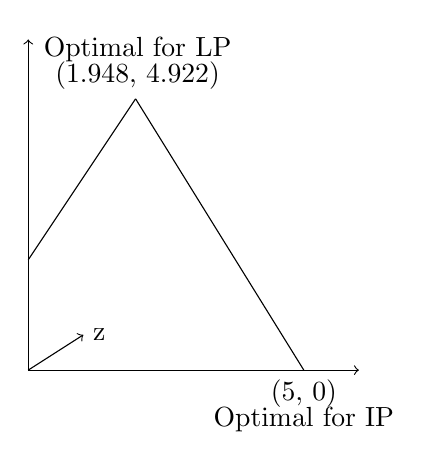
\begin{tikzpicture}[scale=0.7]
                            \draw [->] (1,1) -- (1, 7);
                            \draw [->] (1,1) -- (7, 1);
                            \draw (1,3) -- (2.948, 5.922);
                            \draw (2.948, 5.922) -- (6, 1);
                            \draw [->] (1,1) -- (2, 1.64);
                            \node [right] at (2, 1.64) {z};
                            \node [above] at (2.984, 5.922) {(1.948, 4.922)};
                            \node [above] at (2.984, 6.422) {Optimal for LP};
                            \node [below] at (6,1) {(5, 0)};
                            \node [below] at (6, 0.5) {Optimal for IP};
                        \end{tikzpicture}
                        \caption{Optimal solution for LP / IP}
                    \end{figure}

                \paragraph{QAP example}
                    Rounding can make the LP useless. For example, for QAP problem, the IP model is
                    \begin{align*}
                        \text{min} \quad z &= \sum_{i\in D} \sum_{s\in O} c_{is} x_{is} + \sum_{i\in D} \sum_{j \in D} \sum_{s \in O} \sum_{t\in O} w_{ij}^{st}y_{ij}^{st}  \\
                        \text{s.t.} \quad & \sum_{i \in D} x_{is} =1, \quad s\in O  \\
                                    &\sum_{s \in O} x_{is} = 1, \quad i \in D  \\
                                    &x_{is} \in \{0, 1\}, \quad i \in D, s\in O  \\
                                    & y_{ij}^{st} \ge x_{is} + x_{jt} - 1, \quad i\in D, j\in D, s\in O, t \in O  \\
                                    & y_{ij}^{st} \ge 0, \quad i\in D, j\in D, s\in O, t \in O  \\
                                    & y_{ij}^{st} \le x_{is}, \quad i\in D, j\in D, s\in O, t \in O  \\
                                    & y_{ij}^{st} \le x_{jt}, \quad i\in D, j\in D, s\in O, t \in O  
                    \end{align*}
                    We can get the optimal solution for LP supposing $\forall i, s \quad x_{is}\in [0, 1]$
                    \begin{align*}
                        x_{is} &= \frac{1}{|D|}, \quad i \in D, s\in O   \\
                        y_{ij}^{st} & = 0, \quad i\in D, j\in D, s\in O, t \in O 
                    \end{align*}
                   
            \subsection{Relaxation}

                \paragraph{Local Optimal v.s. Global Optimal}
                    Let 
                    \begin{align*}
                        Z_s &= \text{min} \{f(x):x\in S\} \\
                        Z_t &= \text{min} \{f(x):x\in T\}  \\
                        & S \subset T 
                    \end{align*}
                    then

                    \begin{equation*}Z_t \le Z_s  \end{equation*}
                    Notice that if $x_T^* \in S$ then $x_S^*=x_T^*$, to generalized it, We have

                    \begin{align*}
                        \begin{cases}x_T^* \in \text{arg min} \{f(x): x\in T\} \\ x_T^* \in S\end{cases} \\ \Rightarrow x_T^*\in \text{arg min} \{f(x): x\in S\} 
                    \end{align*}

                    Especially for IP, we can take the LP relaxation as $T$ and the original feasible region of IP as $S$, therefore, if we find an optimal solution from LP relaxation $T$ which is also a feasible solution of $S$, then it is the optimal solution for IP ($S$)
                    
                \paragraph{LP Relaxation}
                    To perform the LP relaxation, we expand the feasible region
                    \begin{align*}
                        x \in \{0,1\} & \rightarrow x\in [0, 1]  \\
                        y\in Z^+ & \rightarrow y \ge 0 
                    \end{align*}
                    If we have $Z_{LP}(s) = conv(s)$ then
                    \begin{equation*} LP(s): {x\in R_+^n: Ax\le b}\end{equation*}
                    The closer $LP(s)$ is to $conv(s)$ the better. Interestingly, we only need to know the convex in the direction of $c$.\\

                    For IP problem
                    \begin{align*}
                        Z_{IP} \quad \text{max} \quad &z = cx  \\
                                \text{s.t.} &Ax \le b \\
                                        &x\in {Z^n} 
                    \end{align*}

                    In feasible region $S = \{x\in Z^n, Ax\le b\}$ , the optimal solution $Z_{IP} = \text{max}\{cx: x\in S\}$. Denote $conv(S)$ as the convex hull of $S$ then

                    \begin{equation*}Z_{IP}(S) = Z_{IP}(conv(S))  \end{equation*}
            
                \paragraph{Relation Between LP Relaxation and IP}
                    Let
                    \begin{align*}
                        Z_{IP} &=\max_{x\in S} cx, \quad \text{where } s \text{ is a set of integer solutions} \\
                        Z_{LP} &=\max cx, \quad \text{the LP relaxation of IP}  
                    \end{align*}
                    then
                    \begin{align*}
                        Z_{IP} &= \max_{1\le i \le k} \{\max_{x \in S_i} cx \} \\
                        \text{iff} \quad S&=\bigcup_{1\le i \le k} S_i 
                    \end{align*}
                    Notice that $S_i$ don\rq{}t need to be disjointed.
                    
                \paragraph{LP feasibility and IP(or MIP) feasibility}
                    Solve the LP relaxation, one of the following things can happen
                    \begin{itemize}
                        \item LP relaxation is infeasible $\rightarrow$ MIP is infeasible
                        \item LP relaxation is unbounded $\rightarrow$ MIP is infeasible or unbounded
                        \item LP relaxation has optimal solution $\hat{x}$ and $\hat{x}$ are integer ($\hat{x} \in S$), $\rightarrow$ $Z_{IP} = Z_{LP}$
                        \item LP relaxation has optimal solution $\hat{x}$ and $\hat{x}$ are not integer ($\hat{x} \notin S$), now defines a new upper bound, $Z_{LP} \ge Z_{IP}$                    
                    \end{itemize}
                    If the first three happens, stop, if the fourth happens, we branch and recursively solve the sub-problems.

        \section{Branch and Bound}

            \subsection{Algorithm overview}
                \begin{algorithm}[H]
                    \caption{Branch and Bound (For maximization problem)}
                    \begin{algorithmic}[1]
                        \State find a feasible solution as the initial Lower bound $L$
                        \State put the original LP relaxation in candidate list $S$
                        \While {$S \ne \emptyset$}
                            \State select a problem $\hat{S}$ from $S$
                            \State solve the LP relaxation of $\hat{S}$ to obtain $u(\hat{S})$
                            \If {LP is infeasible}
                                \State $\hat{S}$ pruned by infeasibility
                            \ElsIf {LP is unbounded}
                                \State \Return Unbounded
                            \ElsIf{LP $u(\hat{S}) \le L$}
                                \State $\hat{S}$ pruned by bound
                            \ElsIf{LP $u(\hat{S}) > L$}
                                \If {$\hat{x}\in S$}
                                    \State $u(\hat{S})$ becomes new $L$, $L=u(\hat{S})$
                                \ElsIf {$\hat{x}\notin S$}
                                    \State branch and add the new sub-problems to $S$
                                    \If {LP $u(\hat{S})$ is at current best upper bound}
                                        \State set $U=u(\hat{S})$
                                    \EndIf
                                \EndIf
                            \EndIf
                        \EndWhile
                        \If {Lower bound exists}
                            \State find the optimal at $L$
                        \Else
                            \State Infeasible
                        \EndIf
                    \end{algorithmic}
                \end{algorithm}

            \subsection{Idea of Divide and Conquer}
                For each iteration, divide the feasible region of LP into two parts (and an infeasible part), solve the LP in those parts.\\
                \begin{figure}[H]
                    \centering
                    \begin{tikzpicture}[scale=0.5]
                        \draw [<->] (10, 0) -- (0,0) -- (0,10);
                        \draw (0, 8.5) -- (10, 2.5);
                        \draw (2, 8) -- (9, 0);
                        \draw [dashed] (3,0) -- (3,10);
                        \draw [dashed] (4,0) -- (4,10);
                        \node at (1.5, 5) {$S_1$};
                        \node at (3.5, 4) {$S_2$};
                        \node at (5, 3) {$S_3$}; 
                    \end{tikzpicture}
                    \caption{Divide and Conquer}
                \end{figure}
                In this iteration, the original feasible region have been partition into three parts, where $S_2$ is infeasible for IP because there is not integer point in it. We continue the iteration for $S_1$ and $S_2$. Each partition is suppose to give a new upper bound / lower bound and reduce the infeasible space.

                If the temp optimal integer in $S_1$ is larger than the LP relaxation in $S_3$, we can cut $S_3$.
                
        \section{Searching, Branching, and Pruning}
            \subsection{Strategies in B\&B}
                \begin{figure}[H]
                    \centering
                    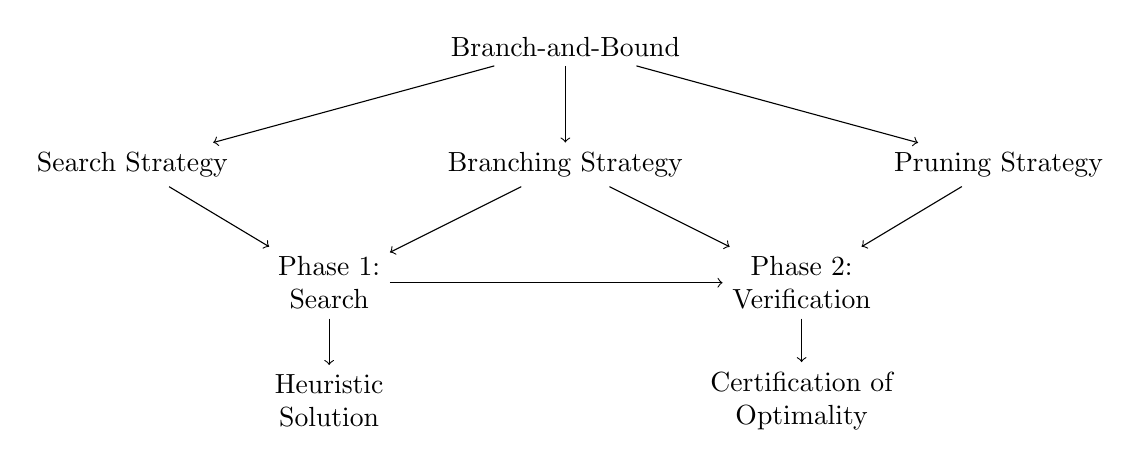
\begin{tikzpicture}[node distance=1.5cm]
                        \node (bb) {Branch-and-Bound};
                        \node (Branching) [below of=bb] {Branching Strategy};
                        \node (Select) [right of=Branching, xshift = -7cm] {Search Strategy};
                        \node (Pruning) [left of=Branching, xshift = 7cm] {Pruning Strategy};
                        \node (Search) [below of=Branching, xshift = -3cm, align=center] {Phase 1:\\Search};
                        \node (Verification) [below of=Branching, xshift = 3cm, align=center] {Phase 2:\\Verification};
                        \node (heu) [below of=Search, align=center] {Heuristic\\Solution};
                        \node (cer) [below of=Verification, align=center] {Certification of\\Optimality};
                        \draw [->] (bb) -- (Select);
                        \draw [->] (bb) -- (Branching);
                        \draw [->] (bb) -- (Pruning);
                        \draw [->] (Select) -- (Search);
                        \draw [->] (Branching) -- (Search);
                        \draw [->] (Branching) -- (Verification);
                        \draw [->] (Pruning) -- (Verification);
                        \draw [->] (Search) -- (Verification);
                        \draw [->] (Search) -- (heu);
                        \draw [->] (Verification) -- (cer);
                    \end{tikzpicture}
                \end{figure}

            \subsection{Search Strategy: Choose Node to Branch}
                \paragraph{Depth-first search}
                    It can be implemented by maintaining the list of unexplored subproblems $L$ as a stack. The algorithm removes the top item from the stack to choose the next subproblem to explore, and when children are generated as a result of branching, they are inserted on the top of $L$. Thus, the next subproblem that is explored is the most recently generated subproblem.

                    \begin{itemize}
                        \item DFS does not need to store the entire list of unexplored subproblems (only stores the path from the root of T to the current subproblem)
                        \item If no unexplored children remain, the algorithm backtracks to the closest ancestor node with unexplored children.
                        \item Use the LP relaxations as lower bounds. The LP solver can often reuse information from the parent LP solution as a starting point for the child LP solution
                        \item Naive implementations of DFS do not use any information about problem structure or bounds
                        \item Search tree is extremely unbalanced
                    \end{itemize}

                \paragraph{Breadth-first search}
                    BFS explores all subproblems that are at a fixed distance from the root before exploring any deeper subproblems.

                    \begin{itemize}
                        \item Finding an optimal solution that is closest to the root of the tree, thus operating well on unbalanced search trees
                        \item Generally unable to exploit pruning rules that compare against the current incumbent solution $\Rightarrow$ high memory
                        \item Best bound search $\Rightarrow$ improve dual bound
                        \item Best estimate search $\Rightarrow$ improve primal bound
                    \end{itemize}

                \paragraph{Best-first search, A* search}
                    makes use of a heuristic measure-of-best function to compute every subproblem by a admissible index $\mu$.

            \subsection{Branching Strategy: Choose Branching Variable}
                % \paragraph{The goal of Branching}
                %     \begin{itemize}
                %         \item Divide the problem into easier subproblems
                %         \item We want to chose the branching variables that minimize the sum of the solution times of the sub-problems
                %         \item If after branching the $u(S_i)$ changes a lot,
                %         \begin{itemize}
                %             \item we can find a good L first
                %             \item the branch may get worse than the current bound first
                %         \end{itemize}
                %         \item Instead of solving the potential two branches for all candidates to optimality, solve a few iterations of the dual simplex, each iteration of pivoting yields an upper bound.
                %     \end{itemize}
                    
                \paragraph{The Most Violated Integrality constraint}
                    Pick the $j$ of which $x_j - \lfloor \hat{x_j} \rfloor$ is the closest to 0.5

                \paragraph{Strong Branching}
                    Select a few candidates $(K)$, create sub-problems for each of these variables, run a few dual simplex iterations to see the improved bounds, select the variable with the best bounds, and then selects for branching the variable that induces the most change in the objective.

                    \begin{itemize}
                        \item Might fix variable, when one side is infeasible
                        \item Detect infeasibility, when both side are infeasible
                        \item Can be speed up by limit the number of iterations, or stop when improvement is found.
                        \item Domain propagation
                    \end{itemize}

                \paragraph{Pseudo-cost Branching}               
                    
                    Pseudo-cost attempts to predict the per-unit change in the objective function for each candidate branching variable, based on past experience in the tree. The basic idea of this strategy is to keep track for each variable $x_i$ the change in the objective function when this variable was previously chosen as the variable to branch on. By branching on a variable that is expected to produce a significant change in the objective function, it is more likely that the generated subproblems can be pruned. One difficulty with pseudocost branching is that no information about past branching behavior is available at the beginning of the algorithm, so the pseudocosts for each variable must be initialized in some way.

                    For variable $x_j\in K$, 
                    
                    \begin{equation*}\begin{cases}P_j^+, & \text{bound reduction if rounded up} \\ P_j^-, & \text{bound reduction if rounded down}\end{cases}\end{equation*}

                    define $f_j = x_j -\lfloor x_j \rfloor$
                    \begin{equation*}\begin{cases}D_j^+ = P_j^+ (1-f_j) \\ D_j^- = P_j^- f_j\end{cases}\end{equation*}

                    \begin{figure}[H]
                        \centering
                        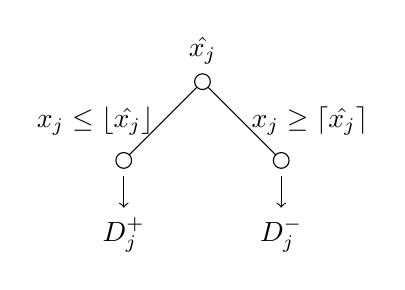
\begin{tikzpicture}[scale=0.2]
                            \draw (0, 5) circle [radius=0.5];
                            \draw (-5, 0) circle [radius=0.5];
                            \draw (5, 0) circle [radius=0.5];
                            \draw (0.353, 4.647) -- (4.647, 0.353);
                            \draw (-0.353, 4.647) -- (-4.647, 0.353);
                            \node [above] at (0, 5.5) {$\hat{x_j}$};
                            \node [left] at (-2.5, 2.5) {$x_j \le \lfloor \hat{x_j} \rfloor$};
                            \node [right] at (2.5, 2.5) {$x_j \ge \lceil \hat{x_j} \rceil$};
                            \draw [->] (-5, -1) -- (-5, -3);
                            \draw [->] (5, -1) -- (5, -3);
                            \node [below] at (-5, -3) {$D_j^+$};
                            \node [below] at (5, -3) {$D_j^-$};
                        \end{tikzpicture}
                        \caption{Strong Branching}
                    \end{figure}

                    For those variables in $K$ find the
                    \begin{itemize}
                        \item $\max \{\min\{ {D_j^+},  {D_j^-}\}\}$, or
                        \item $\max \{\max\{ {D_j^+},  {D_j^-}\}\}$, or
                        \item $\max \{\frac{D_j^+ + D_j^-}{2}\}$, or
                        \item $\max \{\alpha_1\min\{ {D_j^+},  {D_j^-}\} + \alpha_2\max\{ {D_j^+},  {D_j^-}\}\}$
                    \end{itemize}
                    
                    to branch.

            \subsection{Branching Strategy: Create Offspring}

                \paragraph{Traditional Branching}
                    For $\hat{x} \notin S$, $\exists j \in N$ such that

                    \begin{equation*}\hat{x_j} -\lfloor\hat{x_j}\rfloor > 0 \end{equation*}

                    Create two sub-problems

                    \begin{figure}[H]
                        \centering
                        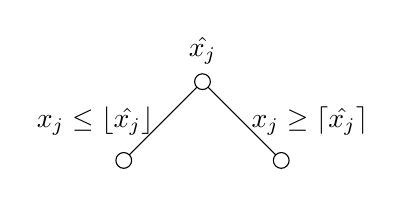
\begin{tikzpicture}[scale=0.2]
                            \draw (0, 5) circle [radius=0.5];
                            \draw (-5, 0) circle [radius=0.5];
                            \draw (5, 0) circle [radius=0.5];
                            \draw (0.353, 4.647) -- (4.647, 0.353);
                            \draw (-0.353, 4.647) -- (-4.647, 0.353);
                            \node [above] at (0, 5.5) {$\hat{x_j}$};
                            \node [left] at (-2.5, 2.5) {$x_j \le \lfloor \hat{x_j} \rfloor$};
                            \node [right] at (2.5, 2.5) {$x_j \ge \lceil \hat{x_j} \rceil$};
                        \end{tikzpicture}
                        \caption{Traditional Branching}
                    \end{figure}

                \paragraph{Constraint Branching}

                    Use parallel constraints to branch, e.g.

                    \begin{figure}[H]
                        \centering
                        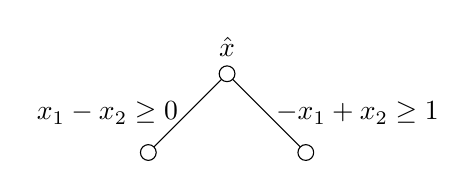
\begin{tikzpicture}[scale=0.2]
                            \draw (0, 5) circle [radius=0.5];
                            \draw (-5, 0) circle [radius=0.5];
                            \draw (5, 0) circle [radius=0.5];
                            \draw (0.353, 4.647) -- (4.647, 0.353);
                            \draw (-0.353, 4.647) -- (-4.647, 0.353);
                            \node [above] at (0, 5.5) {$\hat{x}$};
                            \node [left] at (-2.5, 2.5) {$x_1 - x_2 \ge 0$};
                            \node [right] at (2.5, 2.5) {$-x_1 + x_2 \ge 1$};
                        \end{tikzpicture}
                        \caption{Constraint Branching}
                    \end{figure}
                
                \paragraph{Special Ordered Sets of type 1 (SOS1 or S1)} are a set of variables, at most one of which can take a non-zero value, all others being at 0. 

                    \begin{figure}[H]
                        \centering
                        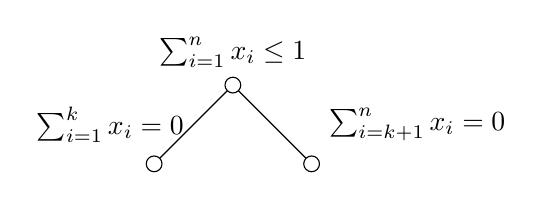
\begin{tikzpicture}[scale=0.2]
                            \draw (0, 5) circle [radius=0.5];
                            \draw (-5, 0) circle [radius=0.5];
                            \draw (5, 0) circle [radius=0.5];
                            \draw (0.353, 4.647) -- (4.647, 0.353);
                            \draw (-0.353, 4.647) -- (-4.647, 0.353);
                            \node [above] at (0, 5.5) {$\sum_{i=1}^{n}x_i\le 1$};
                            \node [left] at (-2.5, 2.5) {$\sum_{i=1}^{k}x_i=0$};
                            \node [right] at (5.5, 2.5) {$\sum_{i=k+1}^{n}x_i=0$};
                        \end{tikzpicture}
                        \caption{SOS1 Branching}
                    \end{figure}

                \paragraph{Special Ordered Sets of type 2 (SOS2 or S2)}: an ordered set of non-negative variables, of which at most two can be non-zero, and if two are non-zero these must be consecutive in their ordering. 

                    \begin{figure}[H]
                        \centering
                        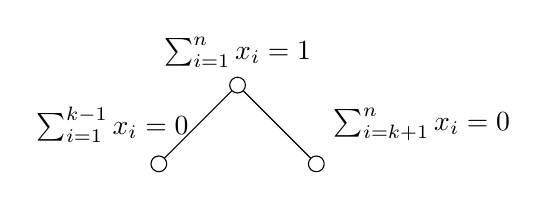
\begin{tikzpicture}[scale=0.2]
                            \draw (0, 5) circle [radius=0.5];
                            \draw (-5, 0) circle [radius=0.5];
                            \draw (5, 0) circle [radius=0.5];
                            \draw (0.353, 4.647) -- (4.647, 0.353);
                            \draw (-0.353, 4.647) -- (-4.647, 0.353);
                            \node [above] at (0, 5.5) {$\sum_{i=1}^{n}x_i = 1$};
                            \node [left] at (-2.5, 2.5) {$\sum_{i=1}^{k-1}x_i = 0$};
                            \node [right] at (5.5, 2.5) {$\sum_{i=k+1}^{n}x_i = 0$};
                        \end{tikzpicture}
                        \caption{SOS2 Branching}
                    \end{figure}
                          
                \paragraph{Ryan-Foster}
                    Ryan-Foster is for Set covering problem. The typical model is
                    \begin{align*}
                        \text{min} \quad & \sum_{i \in C} x_i \\
                        \text{s.t.} \quad & \sum_{i \in C} a_{ij}x_{i} \ge 1, \quad \forall j \in U \\
                                & x_i \in \{0, 1\}, \quad \forall i \in C 
                    \end{align*}
                    For any fractional solution, there are at least two elements $(i,j)$ so that $i$ and $j$ are both partially covered by the same set $S$, but there is another set $T$ that only covers $i$
                    
                    \begin{figure}[H]
                        \centering
                        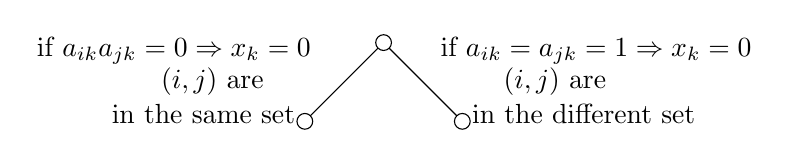
\begin{tikzpicture}[scale=0.2]
                            \draw (0, 5) circle [radius=0.5];
                            \draw (-5, 0) circle [radius=0.5];
                            \draw (5, 0) circle [radius=0.5];
                            \draw (0.353, 4.647) -- (4.647, 0.353);
                            \draw (-0.353, 4.647) -- (-4.647, 0.353);
                            \node [left] at (-7, 2.5) {$(i,j)$ are};
                            \node [left] at (-5, 0.5) { in the same set};
                            \node [left] at (-4, 4.5) {if $a_{ik}a_{jk}=0 \Rightarrow x_k = 0$};
                            \node [right] at (7, 2.5) {$(i,j)$ are};
                            \node [right] at (5, 0.5) { in the different set};
                            \node [right] at (3, 4.5) {if $a_{ik}=a_{jk}=1 \Rightarrow x_k=0$};
                        \end{tikzpicture}
                        \caption{Ryan Foster Branching}
                    \end{figure}

            \subsection{Pruning Rules}
                \paragraph{Lower bound}
                    The most common way to prune is to produce a lower bound on the objective function value at each subproblem, and use this to prune subproblems whose lower bound is no better than the incumbent’s solution value. Lower bounds are computed by relaxing various aspects of the problem.

                    \begin{itemize}
                        \item Many different lower bound can be computed
                        \item Attempt to prune using the easy lower bounds first, then move on to more complex
                        \item One of the ``easy lower bound'' can be LP relaxation
                        \item Another ``easy lower bound'' can be Lagrangian relaxation for IP.
                    \end{itemize}

                \paragraph{Dominance relations}
                    In contrast to lower bounding rules, dominance relations allow subproblems to be pruned if they can be shown to be dominated by some other subproblem. In other words, if subproblem $S_1$ dominates subproblem $S_2$ , this means that for any solution that is a descendant of $S_2$ , there exists a complete solution descending from $S_1$ that is at least as good. 

        \section{Use Branch-and-Bound to Solve Other Problems}
            \paragraph{Close-enough Traveling Salesman Problem}
                Given a set of vertices $V = \{0, 1, \cdots, n\}$ in a 2-dimensional space with coordinates $(\bar{x}, \bar{y}), i = 0, 1, \cdots, n$. Each vertex $i$ is in the center of a convex region bounded by a circle $D_i$ with radius $r_i$. Assume that $(\bar{x}_i, \bar{y}_i) \neq (\bar{x}_j, \bar{y}_j), \forall i, j \in V, i \neq j$. The problem lies in determining the value of the coordinates of the hitting points $(\bar{x}_i, \bar{y}_i) \in \mathbb{R}^2$ and a sequence $L = (k_0, k_1, \cdots, k_n), k_i \in V$ representing the order in which the vertices are covered, such that the tour over the hitting points forms a Hamiltionian cycle of minimum length and $(\bar{x}_i, \bar{y}_i) \in D_i, i \in V$.

            \paragraph{Coutinho et al. 2016} 

                Each branch-and-bound node is associated with an optimal partial tour that needs to visit only a given subset of vertices in a particular order. At the root node, the algorithm chooses three vertices to generate an initial sequence of nodes that need to be visited. Because there are only three vertices involved in this sequence and costs are symmetric, their order will not affect the solution. Therefore, the problem of finding an optimal tour that visits these three vertices in the given order is a valid relaxation of the main problem regardless of the choice of the initial sequence. If the associated solution is feasible, i.e., all customers are covered, then this solution is optimal and the problem is solved. Otherwise, for this root node, the algorithm branches into three subproblems; in each of them, a vertex that does not belong to the tour is inserted in a different position. A node is discarded if its cost is greater than or equal to the best known upper bound or if its associated solution is feasible. Otherwise, a branching is performed over this node using the same rationale applied in the root node. Note that the number of child nodes (subproblems) for every node in the tree is equal to the number of vertices in the partial sequence of the parent node. \citep{Coutinho2016}

                \begin{figure}[H]
                    \centering
                    \includegraphics[width=1\textwidth]{../../image/BnB_CETSP.png}
                    \caption{An example of the B\&B algorithm for an instance with 7 vertices}
                    \label{fig:BnB_CETSP}
                \end{figure}

    \chapter{Special Topic: Formulation Tips}
        \begin{center}
            \textit{``Trick or Treat.''}
        \end{center}

        \section{Linear Program Formulation Tips}
            \paragraph{Absolute Value}
                
                Consider the following model statement:
                \begin{align*}
                    \min \quad & \sum_{j\in J}c_j|x_j|, \quad c_j > 0 \\
                    \text{s.t.} \quad & \sum_{j\in J}a_{ij}x_j \gtreqless b_i, \quad \forall i\in I \\
                                      & x_j \quad \text{unrestricted}, \quad \forall j\in J 
                \end{align*}

                
                Equivalent model:
                \begin{align*}
                    \min \quad & \sum_{j\in J}c_j(x_j^+ + x_j^-), \quad c_j > 0 \\
                    \text{s.t.} \quad & \sum_{j\in J}a_{ij}(x_j^+ - x_j^-) \gtreqless b_i, \quad \forall i\in I \\
                                      & x_j^+, x_j^- \ge 0, \quad \forall j\in J 
                \end{align*}
            
            \paragraph{Minimax Objective}
                
                Consider the following model statement:
                \begin{align*}
                    \min \quad & \max_{k\in K}\sum_{j\in J}c_{kj}x_j \\
                    \text{s.t.} \quad & \sum_{j\in J}a_{ij}x_j \gtreqless b_i, \quad \forall i\in I \\
                                      & x_j \ge 0, \quad \forall j\in J 
                \end{align*}
                
                Equivalent model:
                \begin{align*}
                    \min \quad & z \\
                    \text{s.t.} \quad & \sum_{j\in J}a_{ij}x_j \gtreqless b_i, \quad \forall i\in I \\
                                      & \sum_{j\in J}c_{kj}x_j \le z, \quad \forall k\in K \\
                                      & x_j \ge 0, \quad \forall j\in J 
                \end{align*}
            
            \paragraph{Fractional Objective}
                
                Consider the following model statement:
                \begin{align*}
                    \min \quad & \frac{\sum_{j\in J}c_{j}x_j + \alpha}{\sum_{j\in J}d_{j}x_j + \beta} \\
                    \text{s.t.} \quad & \sum_{j\in J}a_{ij}x_j \gtreqless b_i, \quad \forall i\in I \\
                                      & x_j \ge 0, \quad \forall j\in J 
                \end{align*}
                
                Equivalent model:
                \begin{align*}
                    \min \quad & \sum_{j\in J}c_{j}x_jt + \alpha t \\
                    \text{s.t.} \quad & \sum_{j\in J}a_{ij}x_j \gtreqless b_i, \quad \forall i\in I \\
                                      & \sum_{j\in J}d_jx_jt + \beta t = 1\\
                                      & t > 0 \\
                                      & x_j \ge 0, \quad \forall j\in J \\
                                      & (t = \frac1{\sum_{j\in J}d_jx_j + \beta})
                \end{align*}
            
            \paragraph{Range Constraint}
                
                Consider the following model statement:
                \begin{align*}
                    \min \quad & \sum_{j\in J}c_jx_j \\
                    \text{s.t.} \quad & d_i\le \sum_{j\in J}a_{ij}x_j \le e_i, \quad \forall i\in I \\
                                      & x_j \ge 0, \quad \forall j\in J 
                \end{align*}
                
                Equivalent model:
                \begin{align*}
                    \min \quad & \sum_{j\in J}c_jx_j, \quad c_j > 0 \\
                    \text{s.t.} \quad & u_i + \sum_{j\in J}a_{ij}x_j = e_i, \quad \forall i\in I \\
                                      & x_j \ge 0, \quad \forall j\in J \\
                                      & 0\le u_i \le e_i-d_i, \quad \forall i\in I 
                \end{align*}

        \section{Integer Program Formulation Tips}
            \paragraph{A Variable Taking Discontinuous Values}
                 In algebraic notation: 
                \begin{equation*}
                    x = 0,\quad \text{or} \quad l\le x \le u 
                \end{equation*}
                
                Equivalent model:
                \begin{align*}
                    & x \le uy \\
                    & x \ge ly  \\
                    & y \in \{0, 1\} 
                \end{align*}
                where
                \begin{equation*}y=\begin{cases}0, & \text{if }x=0 \\ 1, & \text{if } l\le x \le u\end{cases} \end{equation*}
                    
            \paragraph{Fixed Costs}
                 In algebraic notation: 
                \begin{equation*}
                    C(x) = \begin{cases} 0 & \text{for } x=0 \\ k + cx & \text{for } x > 0 \end{cases} 
                \end{equation*}
                
                Equivalent model:
                \begin{align*}
                    & C^*(x, y) = ky+cx\\
                    & x \le My  \\
                    & x \ge 0 \\
                    & y \in \{0, 1\} 
                \end{align*}
                where
                \begin{equation*}y=\begin{cases}0, & \text{if }x=0 \\ 1, & \text{if }x\ge 0\end{cases} \end{equation*}
            
            \paragraph{Either-or Constraints}
                 In algebraic notation: 
                \begin{equation*}
                    \sum_{j\in J} a_{1j} x_j \le b_1 \text{ or } \sum_{j\in J} a_{2j} x_j \le b_2 
                \end{equation*}
                
                Equivalent model:
                \begin{align*}
                    & \sum_{j\in J} a_{1j} x_j \le b_1 + M_1y  \\
                    & \sum_{j\in J} a_{2j} x_j \le b_2 + M_1(1-y)  \\
                    & y \in \{0, 1\} 
                \end{align*}
                where
                \begin{equation*}y=\begin{cases}0, & \text{if }\sum_{j\in J} a_{1j} x_j \le b_1 \\ 1, & \text{if } \sum_{j\in J} a_{2j} x_j \le b_2\end{cases} \end{equation*}
                Notice that the sign before $M$ is determined by the inequality $\ge$ or $\le$, if it is \lq\lq{}$\ge$\rq\rq{}, use \lq\lq{}$-$\rq\rq{}, if it \lq\lq{}$\le$\rq\rq{}, use \lq\lq{}+\rq\rq{}.
            
            \paragraph{Conditional Constraints}
                 If constraint A is satisfied, then constraint B must also be satisfied
                \begin{equation*}
                    \text{If} \quad \sum_{j\in J} a_{1j} x_j \le b_1 \text{ then } \sum_{j\in J} a_{2j} x_j \le b_2 
                \end{equation*}
                The key part is to find the opposite of the first condition. We are using $A\Rightarrow B \Leftrightarrow \neg B \Rightarrow \neg A$\\
                Therefore it is equivalent to
                \begin{equation*}
                    \sum_{j\in J} a_{1j} x_j > b_1 \text{ or } \sum_{j\in J} a_{2j} x_j \le b_2 
                \end{equation*}
                Furthermore, it is equivalent to
                \begin{equation*}
                    \sum_{j\in J} a_{1j} x_j \ge b_1 + \epsilon \text{ or } \sum_{j\in J} a_{2j} x_j \le b_2 
                \end{equation*}
                Where $\epsilon$ is a very small positive number.\\
                
                Equivalent model:
                \begin{align*}
                    & \sum_{j\in J} a_{1j} x_j \ge b_1 + \epsilon -  M_2y  \\
                    & \sum_{j\in J} a_{2j} x_j \le b_2 + M_2(1-y)  \\
                    & y \in \{0, 1\} 
                \end{align*} 
            
            \paragraph{Special Ordered Sets}
                SOS1 Description: Out of a set of yes-no decisions, at most one decision variable can be yes. \
                \begin{align*}
                    x_1=1,x_2=x_3&=\dots=x_n=0  \\
                    &\text{or}  \\
                    x_2=1, x_1=x_3&=\dots=x_n=0  \\
                    &\text{or ...} 
                \end{align*} 
                
                Equivalent model:
                \begin{equation*} \sum_{i} x_i = 1, \quad i \in N \end{equation*}
                
                SOS2 Description: Out of a set of binary variables, at most two variables can be nonzero. In addition, the two variables must be adjacent to each other in a fixed order list.\\
                
                Equivalent model:
                If $x_1, x_2, ... , x_n$ is a SOS2, then
                \begin{align*}
                    & \sum_{i=1}^{n} x_i \le 2  \\
                    & x_i + x_j \le 1, \forall i \in \{1, 2,..., n\}, j \in \{i+2, i+3, ..., n\}  \\
                    &x_i \in \{0, 1\}
                \end{align*}
                                
            \paragraph{Piecewise Linear Formulations}
                 The objective function is a sequence of line segments, e.g. $y=f(x), $ consists $k-1$ linear segments going through $k$ given points $(x_1, y_1), (x_2, y_2), ... ,(x_k, y_k)$.\\
                Denote 
                \begin{equation*}d_i=\begin{cases}1, & x\in (x_i, x_{i+1})\\0, & \text{otherwise} \end{cases}\end{equation*}
                Then the objective function is
                \begin{equation*}\sum_{i \in \{1, 2, ..., k-1\}} y = d_if_i(x) \end{equation*} 
                
                Equivalent model: Given that objective function as a piecewise linear formulation, we can have these constraints\\
                \begin{align*}
                    &\sum_{i \in \{1, 2, ..., k-1\}} d_i =1  \\
                    &d_i \in \{0, 1\}, i \in \{1, 2, ..., k-1\}  \\
                    & x = \sum_{i \in \{1, 2, ..., k\}} w_i x_i  \\
                    & y = \sum_{i \in \{1, 2, ..., k\}} w_i y_i  \\
                    & w_1 \le d_1  \\
                    & w_i \le d_{i-1} + d{i}, i \in \{2, 3, ..., k-1\}  \\
                    & w_k \le d_{k-1} 
                \end{align*}
                In this case, $ w_i \in SOS2$ (second definition)       
                                    
            \paragraph{Conditional Binary Variables}
                 Choose at most $n$ binary variable to be 1 out of  $x_1, x_2, ... x_m, m\ge n$\\
                If $n=1$ then it is SOS1.\\
                
                Equivalent model:
                \begin{equation*}
                    \sum_{k\in \{1,2,...,m\}} x_k \le n
                \end{equation*}
                 Choose exactly $n$ binary variable to be 1 out of  $x_1, x_2, ... x_m, m\ge n$\\
                
                Equivalent model:
                \begin{equation*}
                    \sum_{k\in \{1,2,...,m\}} x_k = n
                \end{equation*}
                 Choose $x_j$ only if $x_k = 1$\\
                
                Equivalent model:
                \begin{equation*}x_j = x_k  \end{equation*}
                 \lq\lq{}and\rq\rq{} condition, iff $x_1, x_2, ... , x_m =1$ then $y=1$\\
                
                Equivalent model:
                \begin{align*}
                    & y \le x_i, i\in \{1, 2, ..., m\}  \\
                    & y \ge \sum_{i \in \{1, 2, ..., m\}} x_i - (m - 1) 
                \end{align*}

            \paragraph{Elimination of Products of Variables}
                 For variables $x_1$ and $x_2$,
                \begin{equation*}y = x_1 x_2\end{equation*}
                
                Equivalent model: If $x_1, x_2$ are binary, it is the same as \lq\lq{}and\rq\rq{} condition of binary variables.\\
                If $x_1$ is binary, while $x_2$ is continuous and $0 \le x_2 \le u$, then
                \begin{align*}
                    y &\le ux_1  \\
                    y &\le x_2  \\
                    y &\ge x_2 - u(1- x_1)  \\
                    y &\ge 0 
                \end{align*}
                If both $x_1$ and $x_2$ are continuous, it is non-linear, we can use Piecewise linear formulation to simulate.

    \chapter{Polyhedral Analysis and Cutting Plane Method}
        \begin{center}
            \textit{``Life is a Crystal.''}
        \end{center}
        \section{Preliminaries}
            \subsection{Valid Inequalities and Faces}
                The inequality denoted by $(\pi, \pi_o)$ is called a valid inequality for $P$ if $\pi x \le \pi_0, \forall x \in P$. Note that $(\pi, \pi_0)$ is a valid inequality iff $P$ lies in the half-space $\{x\in \mathbb{R}^n|Ax\le b\}$

                \begin{figure}[H]
                \centering
                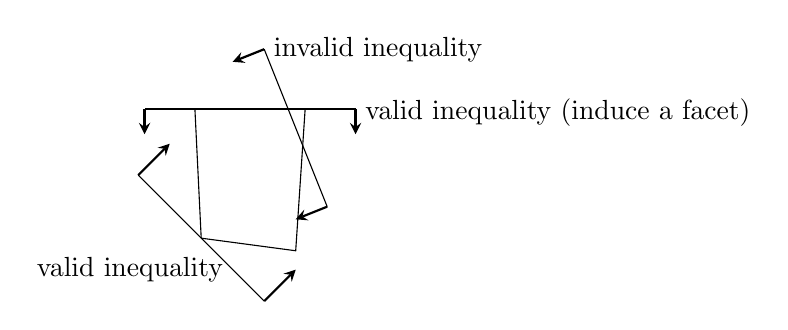
\begin{tikzpicture}[scale=0.4]
                    \draw (0,0) -- (3, -0.4) -- (3.3, 4.1) -- (-0.2, 4.1) -- (0, 0);
                    \draw (-2, 2) -- (2, -2);
                    \draw (4.9, 4.1) -- (-1.8, 4.1);
                    \draw (4, 1) -- (2, 6);
                    \draw [arrow] (-1.8, 4.1) -> (-1.8, 3.3);
                    \draw [arrow] (4.9, 4.1) -> (4.9, 3.3);
                    \draw [arrow] (-2, 2) -> (-1, 3);
                    \draw [arrow] (2, -2) -> (3, -1);
                    \draw [arrow] (4, 1) -> (3, 0.6);
                    \draw [arrow] (2, 6) -> (1, 5.6);
                    \node at (1, -1) [left] {valid inequality};
                    \node at (4.9, 4) [right] {valid inequality (induce a facet)};
                    \node at (2, 6) [right] {invalid inequality};
                \end{tikzpicture}
                \caption{Example of valid/invalid inequality}
                \end{figure}

                \begin{itemize}
                    \item If $(\pi, \pi_0)$ is a valid inequality for $P$ and $F=\{x\in P|\pi x=x_0\}$, $F$ is called a facet of $P$ and we say that $(\pi, \pi_0)$ represents or defines $F$
                    \item A face is said to be proper if $F\ne \emptyset$ and $F\ne P$
                    \item The face represented by $(\pi, \pi_0)$ is nonempty iff $\max \{\pi x |x\in P\}=\pi_0$
                    \item If the face $F$ is nonempty, we say it supports $P$
                    \item Let $P$ be a polyhedron with equality set $M^=$. If
                        \begin{equation*}
                            F=\{x\in P | \pi^T x = \pi_0\}
                        \end{equation*}
                        is not empty, then $F$ is a polyhedron. Let 
                        \begin{equation*}
                            M^= \subseteq M_F^=, M_F^{\le}=M \setminus M_F^= 
                        \end{equation*}
                        then 
                        \begin{equation*}
                            F=\{x | a_i^T x=b_i, \forall i \in M_F^=, a_i^T x \le b_i, \forall i \in M_f^{\le}\}
                        \end{equation*}
                \end{itemize}

            \subsection{Facet}
                \begin{itemize}
                    \item A face $F$ is said to be a facet of $P$ if $dim(F) = dim(P)-1$
                    \item Facets are all we need to describe polyhedral
                    \item If $F$ is a facet of $P$, then in any description of $P$, there exists some inequality representing $F$
                    \item Every inequality that represents a face that is not a facet is unnecessary in the description of $P$
                    \item Every full-dimensional polyhedron $P$ has a unique (up to scalar multiplication) representation that consists of one inequality representing each facet of $P$
                    \item If $dim(P) = n-k$ with $k>0$, then $P$ is described by a maximal set of linearly independent rows of $(A^=, b^=)$, as well as one inequality representing each facet of $P$
                \end{itemize}
                
            \subsection{Proving Facet}
                To prove an inequality $\sum_i a_i x_i \le b_i$ is facet inducing for a $D$ dimensional polyhedral, we need to prove there are $D$ affinely independent vectors in $\sum_i a_i x_i = b_i$

        \section{Some Examples}
            \subsection{Vertices Packing}
                \paragraph{Vertices Packing}
                    Given a graph $G=(V, E)$, with $|V|=n$. A vertices packing solution is that no two neighboring vertices can be chosen at the same time.
                    \begin{equation*}
                        PACK(G) = \{x\in \mathbb{B}^n|x_i + x_j \le 1, \forall (i, j)\in E\} \nonumber
                    \end{equation*}

                    \begin{figure}[!ht]
                        \centering
                        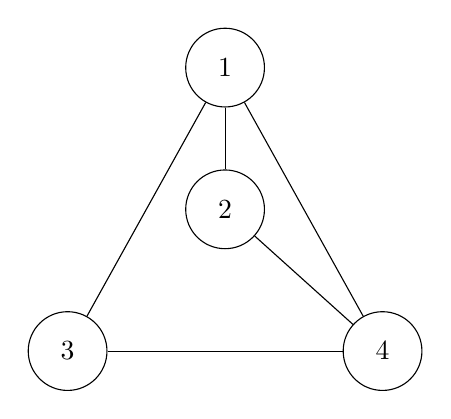
\begin{tikzpicture}[node distance = 1.8cm]
                            \node (1) [branchnode] {1};
                            \node (2) [branchnode, below of=1] {2};
                            \node (3) [branchnode, below of=2, xshift=-2cm] {3};
                            \node (4) [branchnode, below of=2, xshift=2cm] {4};
                            \draw (1) -- (2);
                            \draw (1) -- (3);
                            \draw (1) -- (4);
                            \draw (2) -- (4);
                            \draw (3) -- (4);
                        \end{tikzpicture}
                        \caption{Example of vertices packing problem}
                    \end{figure}

                    The PACK of this graph is

                    \begin{equation*}
                        PACK = conv\left(
                            \left(\begin{matrix}0 \\ 0 \\ 0 \\ 0\end{matrix}\right),
                            \left(\begin{matrix}1 \\ 0 \\ 0 \\ 0\end{matrix}\right),
                            \left(\begin{matrix}0 \\ 1 \\ 0 \\ 0\end{matrix}\right),
                            \left(\begin{matrix}0 \\ 0 \\ 1 \\ 0\end{matrix}\right),
                            \left(\begin{matrix}0 \\ 0 \\ 0 \\ 1\end{matrix}\right),
                            \left(\begin{matrix}0 \\ 1 \\ 1 \\ 0\end{matrix}\right)
                            \right)\nonumber
                    \end{equation*}

                    The dimension of PACK, i.e. $dim(PACK(G))$ is (full-dimensional)
                    \begin{equation*}
                        dim(PACK(G)) = |V| \nonumber
                    \end{equation*}
                    To prove that $dim(PACK(G)) = |V|$, we need to find $|V| + 1$ affinely independent vectors.\\
                    \begin{proof}
                        \begin{equation*}
                            rank\left(\left[\begin{matrix}0 & I_{|V|} \\ 1 & 1\end{matrix}\right]\right) = |V| + 1 \nonumber
                        \end{equation*}
                    \end{proof}                    
                    Therefore, in PACK, $rank(A^=,b^=)=0$ 

                \paragraph{Inequalities and Facets of conv(VP) - Nonnegative Constraints}
                    $x_i \ge 0$ induce facets.\\
                    \begin{proof}
                        \begin{equation*}
                            rank\left(\left[\begin{matrix}0 & 0 \\ 0 & I_{|V|}\end{matrix}\right]\right) = |V| + 1 \nonumber
                        \end{equation*}    
                    \end{proof}               

                \paragraph{Inequalities and Facets of conv(VP) - Neighborhood Constraints}
                    $x_i + x_j \le 1$ is a valid constraint, but it \textbf{DOES NOT} always induce facet.

                \paragraph{Inequalities and Facets of conv(VP) - Odd Hole}
                    Consider a graph $G=(V, E)$, the covering problem is
                    \begin{equation*}
                        \sum_{e\in \delta(i)}x_e \le 1, i\in V, x_e\in \{0, 1\}, e\in E\nonumber
                    \end{equation*}
                    For $T\subset V$, denote $\delta(i)$ as all edges induce to $i\in V$, denote $E(T) \subset E$ as all the edges linked between $(i, j), i\in T, j\in T$, therefore we have
                    \begin{equation*}
                        \sum_{i\in T}\sum_{e\in \delta(i)}x_e \le |T| \nonumber
                    \end{equation*}
                    For edges linking $i \in T, j \in T$, count them twice, for edges linking $i\in T, j\notin T$, count them once.We can have a new constraint
                    \begin{equation*}
                        2\sum_{e\in E(T)}x_e + \sum_{e\in \delta(V\setminus T, T)}x_e \le |T| \nonumber
                    \end{equation*}
                    Perform the Gomory Cut, the following constraint is a valid:
                    \begin{equation*}
                        \sum_{e\in E(T)}x_e \le \lfloor \frac{|T|}2 \rfloor \nonumber
                    \end{equation*}

                    $H$ is an odd hole if it contains circle of $k$ nodes, such that $k$ is odd and there is no cords. e.g. \{1, 2, 5, 6, 3\}. Then, the following inequality is valid,
                    \begin{equation*}
                        \sum_{i\in H}x_i\le \frac{|H|-1}2 \nonumber
                    \end{equation*}
                    Odd Hole inequality \textbf{DOES NOT} always induce facets.

                \paragraph{Inequalities and Facets of conv(VP) - Maximum Clique}
                    A \textbf{clique} is a subset of a graph that in the clique every two vertices linked with each other (complete sub-graph). A \textbf{maximum clique} is a clique that any other vertice can not form a clique with all the points in this clique.

                    $C$ is a maximum clique, then the following inequality is valid and induce a facet,
                    \begin{equation*}
                        \sum_{i\in C} x_i \le 1 \nonumber
                    \end{equation*}
                    
                    \begin{proof}
                        First, if $C=V$
                        \begin{equation*}
                            rank\left(\left[I\right]\right) = |C| = |V| \nonumber           
                        \end{equation*}
                        Second, if $C$ is a subset of $V$, for each vertice in $V \setminus C$, there should be at least one vertice in $C$ that is not linked with it. Therefore for each vertice in $C$ we can find a packing.
                    \end{proof}                    

            \subsection{0-1 Knapsack Problem}
                \paragraph{0-1 Knapsack Problem Formulation}
                    Consider the knapsack set KNAP
                    \begin{equation*}conv(KNAP)= conv(\{x\in \mathbb{B}^n|\sum_{j\in N}a_jx_j\le b\})\end{equation*}
                    in where
                    \begin{itemize}
                        \item $N = \{1, 2, ..., n\}$
                        \item With out lost of generality, assume that $a_j > 0, \forall j \in N$ and $a_j < b, \forall j \in N$
                    \end{itemize}

                \paragraph{Valid Inequalities for a Relaxation}
                    For $P=\{x\in \mathbb{B}^n | Ax\le b\}$, each row can be regard as a Knapsack problem, i.e. for row $i$
                    \begin{equation*}
                        P_i = \{x\in \mathbb{B}^n | a_i^T x \le b_i\} 
                    \end{equation*}
                    is a relaxation of $P$, therefore,
                    \begin{equation*}
                        P\subseteq P_i, \forall i=1,2,...,m 
                    \end{equation*}
                    \begin{equation*}
                        P\subseteq \cap_{i=1}^m P_i 
                    \end{equation*}
                    So any inequality valid for a relaxation of an IP is also valid for IP itself.
                    
                \paragraph{Cover and Extended Cover}
                    A set $C\subseteq N$ is a cover if $\sum_{j\in C} a_j > b$, a cover $C$ is minimal cover if
                    \begin{equation*}
                        C\subseteq N | \sum_{j\in C}a_j > b, \sum_{j\in C\setminus k} a_j \le b, \forall k \in C 
                    \end{equation*}
                    For a cover $C$, we can have the cover inequality
                    \begin{equation*}
                        \sum_{j\in C}x_j \le |C|-1
                    \end{equation*}
                    The inequality is trivial considering the pigeonhole principle. $C\subseteq N$ is a minimal cover, then $E(C)$ is defined as following:
                    \begin{equation*}
                        E(C) = C\cup \{j \in N | a_j \ge a_i, \forall i \in C\}
                    \end{equation*}
                    is called an extended cover. Then we have,
                    \begin{equation*}
                        \sum_{i\in E(C)} x_i \le |C| - 1 \text{ dominates } \sum_{i\in C} x_i \le |C| - 1
                    \end{equation*}
                    and
                    \begin{equation*}
                        \sum_{i\in E(C)} x_i \le |C| - 1 \text{ dominates } \sum_{i\in E(C)} x_i \le |E(C)| - 1
                    \end{equation*}
                    Hereby we need to prove that $\sum_{i\in E(C)} x_i \le |C| - 1$ is valid, by contradiction.\\
                    \begin{proof}
                        Suppose $x^R \in KNAP$, $R$ is a feasible solution, Where
                        \begin{equation*}
                            x^R_j = \begin{cases}1, \quad \text{if $j\in R$} \\ 0, \quad \text{otherwise}\end{cases} 
                        \end{equation*}
                        Then
                        \begin{equation*}
                            \sum_{j\in E(C)}x^R_j \ge |C| \Rightarrow |R \cap E(C)| \ge |C|  
                        \end{equation*}
                        therefore
                        \begin{equation*}
                            \sum_{j\in R}a_j \ge \sum_{j\in R \cap E(C)} a_j \ge \sum_{j\in C} a_j > b 
                        \end{equation*}
                        which means $R$ is a cover, it is contradict to $\sum_{j\in E(C)}x^R_j \ge |C|$ so $x^R \notin KNAP$
                    \end{proof}

                \paragraph{Dimension of KNAP}
                    $conv(KNAP)$ is full dimension, i.e. $dim(conv(KNAP))=n$.\\
                    \begin{proof}
                        $0, e_j, \forall j\in N$ are $n + 1$ affinely independent points in $conv(KNAP)$
                    \end{proof}

                \paragraph{Inequalities and Facets of conv(KNAP) - Lower Bound and Upper Bound Constraints}
                    \begin{itemize}
                        \item $x_k\ge 0$ is a facet of $conv(KNAP)$
                            \begin{proof}
                                $\mathbf{0}, \mathbf{e}_j, \forall j\in N\setminus k$ are $n$ linearly independent vectors that satisfied $x_k = 0$ (thus they are affinely independent), i.e.,
                                \begin{equation*}
                                    rank(\begin{bmatrix}
                                        \textbf{e}_1 & \textbf{e}_2 & \cdots & \textbf{e}_{k - 1} & \textbf{0} & \textbf{e}_{k + 1} & \cdots & \textbf{e}_n
                                    \end{bmatrix}) = |N|
                                \end{equation*}
                            \end{proof}

                        \item $x_k\le 1$ is a facet iff $a_j + a_k \le b, \forall j\in N \setminus k$
                            \begin{proof}
                                $\textbf{e}_k, \textbf{e}_j+\textbf{e}_k, \forall j \in N\setminus k$ are $n$ affinely independent points that satisfied $x_k = 1$, i.e.,
                                \begin{equation*}
                                    rank(\begin{bmatrix}
                                        \mathbf{e}_{1, k} & \mathbf{e}_{2, k} & \cdots & \mathbf{e}_{k - 1, k} & \mathbf{e}_k & \mathbf{e}_{k, k + 1} & \cdots & \mathbf{e}_{k, n}
                                    \end{bmatrix}) = |N|
                                \end{equation*}
                            \end{proof}
                    \end{itemize}                

                \paragraph{Inequalities and Facets of conv(KNAP) - Extended Cover}
                    Order the variables so that $a_1 \ge a_2 \ge \dots \ge a_n$, therefore $a_1 = a_{max}$. Let $C$ be a cover with $\{j_1, j_2, \dots, j_r\}$ where $j_1 < j_2 < \dots < j_r$ so that $a_{j_1} \ge a_{j_2} \ge \dots \ge a_{j_r}$, then
                    \begin{equation*}
                        \sum_{j\in E(C)} x_j \le |C| - 1 
                    \end{equation*}

                    is a facet of $conv(KNAP)$ if
                    \begin{itemize}               
                        \item $C = N$
                            \begin{proof}
                                \begin{equation*}
                                    rank(\begin{bmatrix}
                                        0 & 1 & 1 & \cdots & 1 \\
                                        1 & 0 & 1 & \cdots & 1 \\
                                        1 & 1 & 0 & \cdots & 1 \\
                                        \vdots & \vdots & \vdots & & \vdots\\
                                        1 & 1 & 1 & \cdots & 0
                                        \end{bmatrix}) = |N|
                                \end{equation*}
                            \end{proof}

                        \item $E(C) = N$ and $\sum_{j\in C \setminus \{j_1, j_2\}} a_j + a_{max} \le b$
                            \begin{proof}
                                 ($j_1, j_2$ are two heaviest elements in $C$)
                                \begin{equation*}
                                    rank(\left[\begin{array}{c c c c | c c c}
                                        0 & 1 & \cdots & 1 & 0 & \cdots & 0 \\
                                        1 & 0 & \cdots & 1 & 0 & \cdots & 0 \\
                                        \vdots & \vdots & & \vdots & \vdots & & \vdots\\
                                        1 & 1 & \cdots & 0 & 1 & \cdots & 1 \\
                                        \hline
                                        0 & 0 & \cdots & 0 & 1 & \cdots & 0 \\
                                        \vdots & \vdots & & \vdots & \vdots & & \vdots\\
                                        0 & 0 & \cdots & 0 & 0 & \cdots & 1
                                        \end{array}\right]) = |N|
                                \end{equation*}
                                In $|C|$ rows, select $|C| - 1$ decision variables to be 1. In $|N| - |C|$ rows, select all decision variables in $C$ except for the two with largest weight to be 1 and select one decision variable outside $C$ to be 1.
                            \end{proof} 

                        \item $C = E(C)$ and $\sum_{j\in C \setminus j_1} a_j + a_p \le b$, where $p = \max\{j | j\in N \setminus E(C)\}$
                            \begin{proof}
                                ($j_1$ is the heaviest element in $C$, $k$ is the lightest element outside extended cover)
                                \begin{equation*}
                                    rank(\left[\begin{array}{c c c c | c c c}
                                        0 & 1 & \cdots & 1 & 0 & \cdots & 0 \\
                                        1 & 0 & \cdots & 1 & 1 & \cdots & 1 \\
                                        \vdots & \vdots & & \vdots & \vdots & & \vdots\\
                                        1 & 1 & \cdots & 0 & 1 & \cdots & 1 \\
                                        \hline
                                        0 & 0 & \cdots & 0 & 1 & \cdots & 0 \\
                                        \vdots & \vdots & & \vdots & \vdots & & \vdots\\
                                        0 & 0 & \cdots & 0 & 0 & \cdots & 1
                                        \end{array}\right]) = |N|
                                \end{equation*}
                                In $|C|$ rows, select $|C| - 1$ decision variables to be 1. In $|N| - |C|$ rows, select all decision variables in $C$ except for the one with largest weight to be 1 and select one decision variable outside $C$ to be 1.
                            \end{proof}

                        \item $C \subset E(C) \subset N$ and $\sum_{j\in C \setminus \{j_1, j_2\}} a_j + a_{max} \le b$ and $\sum_{j\in C \setminus j_1} a_j + a_p \le b$
                            \begin{proof}
                                \begin{equation*}
                                    rank(\left[\begin{array}{c c c c | c c c | c c c}
                                        0 & 1 & \cdots & 1 & 0 & \cdots & 0 & 0 & \cdots & 0 \\
                                        1 & 0 & \cdots & 1 & 0 & \cdots & 0 & 1 & \cdots & 1 \\
                                        \vdots & \vdots & & \vdots & \vdots & & \vdots & \vdots & & \vdots \\
                                        1 & 1 & \cdots & 0 & 1 & \cdots & 1 & 1 & \cdots & 1\\
                                        \hline
                                        0 & 0 & \cdots & 0 & 1 & \cdots & 0 & 0 & \cdots & 0\\
                                        \vdots & \vdots & & \vdots & \vdots & & \vdots & \vdots & & \vdots \\
                                        0 & 0 & \cdots & 0 & 0 & \cdots & 1 & 0 & \cdots & 0 \\
                                        \hline
                                        0 & 0 & \cdots & 0 & 0 & \cdots & 0 & 1 & \cdots & 0 \\
                                        \vdots & \vdots & & \vdots & \vdots & & \vdots & \vdots & & \vdots \\
                                        0 & 0 & \cdots & 0 & 0 & \cdots & 0 & 0 & \cdots & 1 \\
                                        \end{array}\right]) = |N|
                                \end{equation*}
                                In the first $|C|$ rows, select $|C| - 1$ decision variables to be 1. In the next $|E(C)| - C$ rows, select all decision variables in $C$ except for two with largest coefficient to be 1, select a decision variable that is in $E(C)$ but not in $C$ to be 1. In the last $|N| - |E(C)|$ row, select all decision variables in $C$ except for the one with largest coefficient to be 1, select a decision variable outside $E(C)$ to be 1.
                            \end{proof}
                    \end{itemize}

        \section{Generic Cutting Planes}
            \subsection{General Approach}
                \paragraph{Cutting Planes}
                \begin{itemize}
                    \item Cutting planes are referred to inequalities valid for $conv(S)$, but which is violated by the solution obtained by solving the current LP relaxation.
                    \item Cutting plane methods attempt to improve the bound produced by the LP relaxation by iteratively adding cutting planes to the initial LP relaxation.
                    \item Adding such inequalities to the LP relaxation may improve the bound (this is not a guarantee).
                \end{itemize}

                \paragraph{Separation Problem} Given a polygon $P \in \mathbb{R}^n$ and $\mathbf{x}^* \in \mathbb{R}^n$, determine whether $\mathbf{x}^* \in P$, and if not, determine $(\mathbf{\pi}, \pi_0)$, a valid inequality for $P$ such that $\mathbf{\pi} \mathbf{x}^* \ge \pi_0$

            \subsection{Generic Cutting Planes}
                \paragraph{Observation}
                    For integer program over a set of variables $x_1, x_2, \cdots, x_n \in \mathbb{Z}_+$
                    \begin{itemize}
                        \item If $\mathbf{ax} = \mathbf{b}$ is a constraint of $P$, then $\mathbf{ax \le b}$ is a valid constraint of $P$
                        \item Suppose there are two valid constraints
                            \begin{align*}
                                a_{11} x_1 + a_{12} x_2 + \cdots + a_{1n} x_n \le b_1
                            \end{align*}
                            and
                            \begin{align*}
                                a_{21} x_2 + a_{22} x_2 + \cdots + a_{2n} x_n \le b_2
                            \end{align*}
                            then
                            \begin{align*}
                                & u_1 (a_{11} x_1 + a_{12} x_2 + \cdots + a_{1n} x_n)\\
                              + & u_2 (a_{21} x_2 + a_{22} x_2 + \cdots + a_{2n} x_n) \\
                                & \qquad \qquad \qquad \qquad \qquad \le u_1 b_1 + u_2 b_2
                            \end{align*}
                            is a valid inequality for $P$
                        \item If $a \le b$ and $a$ is an integer number, then $a \le \floor{b}$
                        \item $x_i \in \mathbb{Z}_+ \Rightarrow -x_i \le 0$
                        \item WLOG, assume $\forall a_i$ in constraint $\sum_{i=1}^n a_i x_i \le b$, $a_i$ is a fractional number. Let $f_i = a_i - \floor{a_i}$ be the fractional part, and $f_i \ge 0$. Then,
                        \begin{equation*}
                            \sum_{i=1}^n a_i x_i - \sum_{i=1}^n f_i x_i \le b - 0
                        \end{equation*}
                        $\Rightarrow$
                        \begin{equation*}
                            \sum_{i=1}^n \floor{a_i} x_i \le \floor{b}
                        \end{equation*} is a valid inequality for $P$.
                    \end{itemize}
                    
                \paragraph{Chv\'atal-Gomory Rounding Method}
                    Let $X = P \cap \mathbb{Z}^n$ be the feasible set of an integer program, where
                    \begin{equation*}
                        P = \{\mathbf{x} \in \mathbb{R}^n | \mathbf{Ax}\le \mathbf{b}, \mathbf{x} \ge 0\}
                    \end{equation*}
                    Also let $\mathbf{a}_i$ be the $i$th column of $\mathbf{A}$, then
                    \begin{equation*}
                        \sum_{i = 1}^n \mathbf{u} \mathbf{a}_i x_i \le \mathbf{ub}
                    \end{equation*}
                    is a valid inequality for $P$ for $u \ge 0$, then
                    \begin{equation*}
                        \sum_{i = 1}^n \floor{\mathbf{u} \mathbf{a}_i} x_i \le \mathbf{ub}
                    \end{equation*}
                    is a valid inequality for $P$, then
                    \begin{equation*}
                        \sum_{i = 1}^n \floor{\mathbf{u} \mathbf{a}_i} x_i \le \floor{\mathbf{ub}}
                    \end{equation*}
                    is a valid inequality for $P$, since $x_i$ is an integer. Such procedures are called Chv\'atal-Gomory rounding procedure, and such cuts are called Chv\'atal-Gomory Cuts.

                \paragraph{Example 1}
                    Let $P$ be
                    \begin{align*}
                        2 x_1 + 3 x_2 &\le 5\\
                        -x_1 + x_2 &\le 2\\
                        x_1, x_2 &\ge 0
                    \end{align*}
                    Then
                    \begin{equation*}
                        \mathbf{A} = \begin{bmatrix}2 & 3 \\ -1 & 1\end{bmatrix} \Rightarrow \mathbf{a}_1 = \begin{bmatrix}2 \\ -1\end{bmatrix}, \mathbf{a}_2 = \begin{bmatrix}3 \\ 1\end{bmatrix}
                    \end{equation*}
                    Let
                    \begin{equation*}
                        \mathbf{u} = \begin{bmatrix}1/2 & 1/3\end{bmatrix}
                    \end{equation*},
                    then
                    \begin{equation*}
                        \begin{bmatrix}1/2 & 1/3\end{bmatrix} \begin{bmatrix}2 \\ -1\end{bmatrix} x_1 + \begin{bmatrix}1/2 & 1/3\end{bmatrix} \begin{bmatrix}3 \\ 1\end{bmatrix} x_2 \le \begin{bmatrix}1/2 & 1/3\end{bmatrix} \begin{bmatrix}5 \\ 2\end{bmatrix}
                    \end{equation*}
                    which is
                    \begin{equation*}
                        \frac{2}{3} x_1 + \frac{11}{6} x_2 \le \frac{19}{6}
                    \end{equation*}
                    then, 
                    \begin{equation*}
                        \floor{\frac{2}{3}} x_1 + \floor{\frac{11}{6}} x_2 \le \floor{\frac{19}{6}} \Rightarrow x_2 \le 3
                    \end{equation*}

                \paragraph{Example 2}
                    Let $P$ be
                    \begin{align*}
                        7 x_1 - 2x_2 &\le 14\\
                        x_2 &\le 3\\
                        2 x_1 - 2x_2 &\le 3\\
                        x_1, x_2 &\ge 0
                    \end{align*}

                    Let $u = \begin{bmatrix}\frac{2}{7} & \frac{37}{63} & 0\end{bmatrix}$

                    Then $2 x_1 + \frac{1}{63} x_2 \le \frac{185}{21} \Rightarrow x_1 \le 4$

                \paragraph{Observation}
                    \begin{itemize}
                        \item It is possible to generate $conv(X)$ using C-G procedures
                        \item The crux lies on the choice of $\mathbf{u}$
                        \item The number of iterations can be huge
                        \item Nevertheless, the procedure has been proven to work well in practice in recent years to generate good inequalities
                        \item One can try generating random multipliers and test the method
                    \end{itemize}

            \subsection{Gomory Cuts}
                Gomory cutting planes can also be derived directly from the tableau while solving an LP relaxation. Consider the set
                \begin{equation*}
                    P = \{(\mathbf{x, s}) \in \mathbb{Z}_+^{n + m}| \mathbf{Ax + Is = b}\}
                \end{equation*}
                in which the LP relaxation of an ILP is put in standard form. Assume for $A$, all the coefficients are integers, so that the slack variables are integers. Clearly,
                \begin{equation*}
                    \mathbf{B^{-1}Ax + B^{-1}Is = B^{-1}b}
                \end{equation*}
                Let $\mathbf{\lambda} = \mathbf{B^{-1}}_j$, then we obtain
                \begin{equation*}
                    \sum_{j = 1}^n \mathbf{\lambda A_j} x_j + \sum_{i = 1}^m \mathbf{\lambda}_i s_i = \mathbf{\lambda b}
                \end{equation*}
                where $\mathbf{A}_j$ is the $j$th column of $\mathbf{A}$ and $\mathbf{\lambda}$ is a row if $\mathbf{B}^{-1}$. Then, the Gomory cut is define by
                \begin{equation*}
                    \sum_{j = 1}^n (\mathbf{\lambda A}_j - \floor{\mathbf{\lambda A}_j}) x_j + \sum_{i = 1}^m (\mathbf{\lambda}_i - \floor{\mathbf{\lambda}_i}) s_i \ge \mathbf{\lambda b} - \floor{\mathbf{\lambda b}}
                \end{equation*}
                Gomory cut is a Chv\'atal-Gomory cut with weights $\mathbf{u}_i = \mathbf{\lambda}_i - \floor{\mathbf{\lambda}_i}$.

                \paragraph{Example}
                    For the following IP
                    \begin{align*}
                        \max \quad & 2 x_1 + 5 x_2\\
                        \text{s.t.} \quad & 4 x_1 + x_2 \le 28\\
                        & x_1 + 4 x_2 \le 27\\
                        & x_1 - x_2 \le 1\\
                        & x_1, x_2 \in \mathbb{Z}_+
                    \end{align*}

                    The optimal tableau of the LP relaxation is as follows

                    \begin{table}[H]
                        \centering
                        \begin{tabular}{c|ccccc|c}
                            & $x_1$ & $x_2$ & $s_1$ & $s_2$ & $s_3$ & RHS\\
                            \hline
                            $x_2$ & 0 & 1 & -2/30 & 8/30 & 0 & 16/3\\
                            $s_3$ & 0 & 0 & -1/3 & 1/3 & 1 & 2/3\\
                            $x_1$ & 1 & 0 & 8/30 & -2/30 & 0 & 17/3
                        \end{tabular}
                    \end{table}

                    For the first row, the Gomory cut is
                    \begin{equation*}
                        \frac{28}{30} s_1 + \frac{8}{30} s_2 \ge \frac{1}{3}
                    \end{equation*}
                    Replace the slack variables, we have
                    \begin{equation*}
                        4 x_1 + 2 x_2 \le 33
                    \end{equation*}

                    For the second row, the Gomory cut is
                    \begin{equation*}
                        \frac{2}{3} s_1 + \frac{1}{3} s_2 \le \frac{2}{3}
                    \end{equation*}

                    Replace the slack variables, we have
                    \begin{equation*}
                        3 x_1 + 2 x_2 \le 27
                    \end{equation*}

                    For the third row, the Gomory cut is
                    \begin{equation*}
                        \frac{8}{30}s_1 + \frac{28}{30}s_2 \ge \frac{2}{3}
                    \end{equation*}

                    Replace the slack variables, we have
                    \begin{equation*}
                        x_1 + 2 x_2 \le 16
                    \end{equation*}

                    This picture shows the effect of adding all Gomory cuts in the first round
                    \begin{figure}[!h]
                        \centering
                        \includegraphics[width=0.6\textwidth]{../../image/CG.png}
                    \end{figure}

        \section{Branch and Cut}
            \paragraph{Two types of valid inequalities}
                The structural constraints are 
                \begin{itemize}
                    \item while this is not a standard term used in mathematical programming, we will use it in reference to the constraints that define a formulation
                    \item these are constraints needs to define the problem. If removed, some infeasible integer solutions may become part of the solution space
                \end{itemize}

                The cutting planes are
                \begin{itemize}
                    \item these are valid constraints that are not needed to define the problem but can be added to tighten the LP relaxation of a formulation
                    \item in other words, they are used for trying to obtain a better LP bound
                \end{itemize}

            \paragraph{User cuts}
                \begin{figure}[H]
                    \centering
                    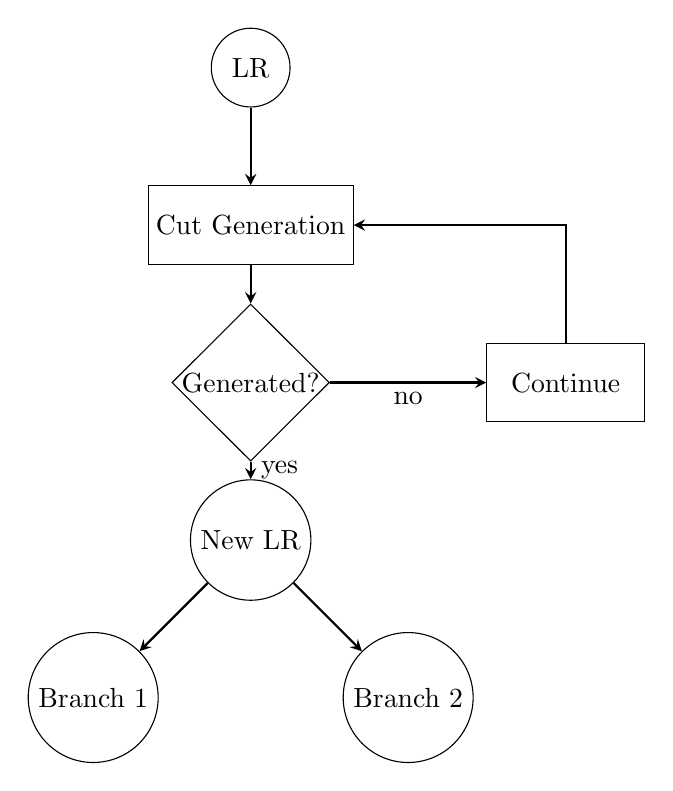
\begin{tikzpicture}[node distance = 2cm]
                        \node (LR) [branchnode] {LR};
                        \node (CG) [process, below of=LR] {Cut Generation};
                        \node (CLimit) [decision, below of=CG] {Generated?};
                        \node (Cont) [process, below of=CG, xshift=4cm] {Continue};
                        \node (NLR) [branchnode, below of=CLimit] {New LR};
                        \node (LNLR) [branchnode, below of=NLR, xshift=-2cm] {Branch 1};
                        \node (RNLR) [branchnode, below of=NLR, xshift=2cm] {Branch 2};
                        \draw [arrow] (LR) -- (CG);
                        \draw [arrow] (CG) -- (CLimit);
                        \draw [arrow] (CLimit) -- node [right] {yes} (NLR);
                        \draw [arrow] (CLimit) -- node [below] {no} (Cont);
                        \draw [arrow] (Cont) |- (CG);
                        \draw [arrow] (NLR) -- (LNLR);
                        \draw [arrow] (NLR) -- (RNLR);
                    \end{tikzpicture}
                    \caption {Branch and Cut for Optional Inequality}\label{OptInq}
                \end{figure}

                Consider the vertice packing problem, we have mentioned that the maximum cliques can be used for adding valid inequalities, this is how it works

                \begin{itemize}
                    \item Given a fractional solution $\hat{x}$, we can find a clique for which $\sum_{i \in C} x_i \le 1, C \in Clique(G)$ is violated
                    \item Solve the following separation problem
                    \begin{align*}
                        \max \quad & \gamma = \sum_{i \in V} \hat{x}_i z_i\\
                        \text{s.t.} \quad & z_i + z_j \le 1, \{i, j\} \notin E\\
                        &z_i \in \{0, 1\}, i \in V
                    \end{align*}
                    \item if $\gamma > 1$ add the clique cut associate with $C$.
                \end{itemize}

            \paragraph{Lazy cuts}
                A typical example for lazy cuts is the DFJ sub-tour elimination for TSP. We will discuss later in this semester.

                \begin{figure}[H]
                    \centering
                    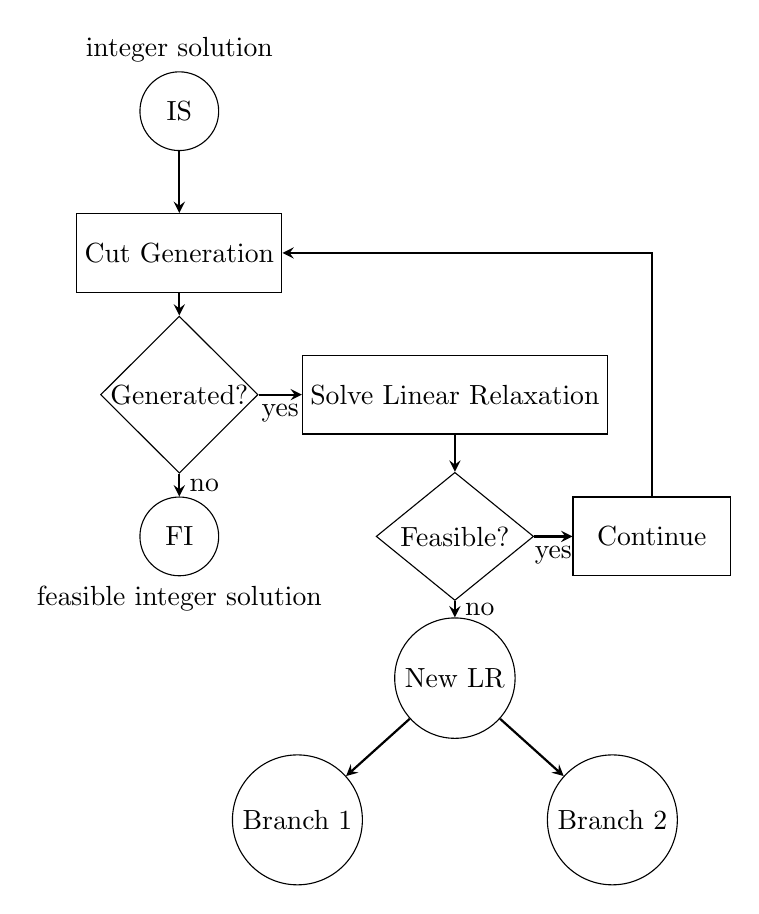
\begin{tikzpicture}[node distance = 1.8cm]
                        \node (IS) [branchnode, label = above:integer solution] {IS};
                        \node (CG) [process, below of=IS] {Cut Generation};
                        \node (CLimit) [decision, below of=CG] {Generated?};
                        \node (FI) [branchnode, below of=CLimit, label = below:feasible integer solution] {FI};
                        \node (LP) [process, below of=CG, xshift = 3.5cm] {Solve Linear Relaxation};
                        \node (LPF) [decision, below of=LP] {Feasible?};
                        \node (NLR) [branchnode, below of=LPF] {New LR};
                        \node (LNLR) [branchnode, below of=NLR, xshift=-2cm] {Branch 1};
                        \node (RNLR) [branchnode, below of=NLR, xshift=2cm] {Branch 2};
                        \node (Cont) [process, below of=LP, xshift=2.5cm] {Continue};
                        \draw [arrow] (IS) -- (CG);
                        \draw [arrow] (CG) -- (CLimit);
                        \draw [arrow] (CLimit) -- node [right] {no} (FI);
                        \draw [arrow] (CLimit) -- node [below] {yes} (LP);
                        \draw [arrow] (LP) -- (LPF);
                        \draw [arrow] (LPF) -- node [right] {no} (NLR);
                        \draw [arrow] (LPF) -- node [below] {yes} (Cont);
                        \draw [arrow] (NLR) -- (LNLR);
                        \draw [arrow] (NLR) -- (RNLR);
                        \draw [arrow] (Cont) |- (CG);
                    \end{tikzpicture}
                    \caption {Branch and Cut for Essential Inequality}\label{EssInq}
                \end{figure}

    \chapter{Graph Algorithm}
        \begin{center}
            \textit{``You can't visit all seven bridges in Königsberg without repetition.''}
        \end{center}

        \section{Preliminaries}
            \subsection{Graphs and Subgraphs}
                \paragraph{Graphs}
                    \begin{definition}[Graph]
                        A \textbf{graph} G consists of a finite set $V(G)$ on vertices, a finite set $E(G)$ on edges and an \textbf{incident relation} than associates with any edge $e\in E(G)$ an unordered pair of vertices not necessarily distinct called \textbf{ends}.
                    \end{definition}

                    \begin{example}
                        The following graph can be represented as
                        \begin{align*}
                            V &= V(G) = \{v_1, v_2, v_3, v_4, v_5, v_6\} \\
                            E &= E(G) = \{e_1, e_2, e_3, e_4, e_5, e_6, e_7, e_8\}\\
                            e_1 &= v_1v_2, \quad e_2 = v_2v_4, \quad \dots
                        \end{align*}

                        \begin{figure}[H]
                            \centering
                            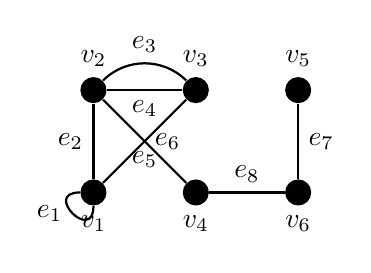
\begin{tikzpicture}[node distance = 1.3 cm]
                                \node (v_2) [solidNode, label=above:{$v_2$}] {};
                                \node (v_3) [solidNode, label=above:{$v_3$}, right of = v_2] {};
                                \node (v_1) [solidNode, label=below:{$v_1$}, below of = v_2] {};
                                \node (v_4) [solidNode, label=below:{$v_4$}, below of = v_3] {};
                                \node (v_5) [solidNode, label=above:{$v_5$}, right of = v_3] {};
                                \node (v_6) [solidNode, label=below:{$v_6$}, below of = v_5] {};
                                \draw [link] (v_2) -- node [left] {$e_2$} (v_1);
                                \draw [link] (v_2) -- node [below] {$e_5$} (v_4);
                                \draw [link] (v_1) to [out = 180, in = 270, looseness = 5] node [left] {$e_1$} (v_1);
                                \draw [link] (v_2) to [out = 45, in = 135] node [above] {$e_3$} (v_3);
                                \draw [link] (v_2) -- node [below] {$e_4$} (v_3);
                                \draw [link] (v_3) -- node [right] {$e_6$} (v_1);
                                \draw [link] (v_5) -- node [right] {$e_7$} (v_6);
                                \draw [link] (v_4) -- node [above] {$e_8$} (v_6);
                            \end{tikzpicture}
                        \end{figure}
                    \end{example}

                    \begin{definition}[Adjacent]
                        Two edges of a graph are \textbf{adjacent} if they have a common end, two vertices are \textbf{adjacent} if they are jointed by an edge.
                    \end{definition}

                    Saving a graph in computer program can be implemented in the following ways:
                    \begin{itemize}
                        \item Adjacency matrix: $m \times n$ matrix, for $A[u, v] = 1$ if $(u, v) \in E$ and $A[u, v] = 0$ otherwise
                        \item Linked list: For every vertex $v$, there is a linked list containing all neighbors of $v$.
                    \end{itemize}
                    Assuming we are dealing with undirected graphs, $n$ is the number of vertices, $m$ is the number of edges, $n - 1 \le m \le n(n-1)/2$, $d_v$ is the number of neighbors of $v$ then
                    \begin{table}[H]
                        \centering
                        \begin{tabular}{|c|c|c|}
                            \hline
                             & Matrix & Linked lists\\
                            \hline
                            memory usage & $O(n^2)$ & $O(m)$\\
                            \hline
                            time to check $(u, v) \in E$ & $O(1)$ & $O(d_u)$\\
                            \hline
                            time to list all neighbors of $v$ & $O(n)$ & $O(d_v)$\\
                            \hline
                        \end{tabular}
                    \end{table}

                \paragraph{Subgraphs}
                    \begin{definition}[Subgraph]
                        Given two graphs $G$ and $H$, $H$ is a \textbf{subgraph} of $G$ if $V(H)\subseteq V(G)$, $E(H)\subseteq E(G)$ and an edge has the same ends in $H$ as it does in $G$. Furthermore, if $E(H)\neq E(G)$ then $H$ is a proper subgraph.
                    \end{definition}

                    \begin{definition}[Vertex-induced, Edge-induced]
                        For a subset $V^\prime \subseteq V(G)$ we define an \textbf{vertex-induced} subgraph $G[V^\prime ]$ to be the subgraph with vertices $V^\prime$ and those edges of $G$ having both ends in $V^\prime$. The \textbf{edge-induced} subgraph $G[E^\prime ]$ has edges $E^\prime$ and those vertices of $G$ that are ends to edges in $E^\prime$.
                    \end{definition}

                    If we combine node-induced or edge-induced subgraphs $G(V^\prime )$ and $G(V - V^\prime )$, we cannot always get the entire graph.

                    \begin{definition}[Degree]
                        Let $v\in V(G)$, then the \textbf{degree} of $v\in V(G)$ denote by $d_G(v)$ is defines to be the number of edges incident of $v$. Loops counted twice.
                    \end{definition}

                    \begin{theorem}
                        For any graph $G=(V, E)$
                        \begin{equation*}
                            \sum_{v\in V}d(v) = 2|E|
                        \end{equation*}
                    \end{theorem}

                    \begin{proof}
                        $\forall$ edge $e=uv$ with $u \neq v$, $e$ is counted once for $u$ and once for $v$, a total of two altogether. If $e=uu$, a loop, then it is counted twice for $u$.
                    \end{proof}

                    \begin{corollary}
                        Every graph has an even number of odd degree vertices.
                    \end{corollary}

                    \begin{proof}
                        \begin{equation*}
                            V = V_E\cup V_O \Rightarrow 
                            \sum_{v\in V}d(v) = \sum_{v\in V_E} d(v) + \sum_{v\in V_O}d(v) = 2|E|
                        \end{equation*}
                    \end{proof}

                \paragraph{Special graphs}
                    \begin{definition}[Complete Graph]
                        A \textbf{complete} graph $K_n (n \ge 1)$ is a simple graph with $n$ vertices and with exactly one edge between each pair of distinct vertices.
                    \end{definition}

                    \begin{definition}[Cycle Graph]
                        A \textbf{cycle} graph $C_n (n \ge 3)$ consists of $n$ vertices $v_1, ... v_n$ and $n$ edges $\{v_1, v_2\}, \{v_2, v_3\}, ... \{v_{n-1}, v_n\}$
                    \end{definition}

                    \begin{definition}[Wheel Graph]
                        A \textbf{wheel} graph $W_n (n \ge 3)$ is a simple graph obtains by adding one vertex to the cycle graph $C_n$, and connecting this new vertex to all vertices of $C_n$ 
                    \end{definition}

                    \begin{definition}[Bipartite Graph]
                        A simple graph is said to be \textbf{bipartite} if the vertex set can be expressed as the union of two disjoint non-empty subsets $V_1$ and $V_2$ such that every edges has one end in $V_1$ and another end in $V_2$
                    \end{definition}

                    \begin{example}
                        Here is an example for bipartite graph
                        \begin{figure}[H]
                            \centering
                            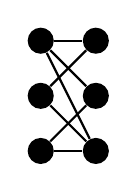
\begin{tikzpicture}[node distance = 0.7 cm]
                                \node (A) [solidNode] {};
                                \node (B) [solidNode, right of = A] {};
                                \node (C) [solidNode, below of = A] {};
                                \node (D) [solidNode, right of = C] {};
                                \node (E) [solidNode, below of = C] {};
                                \node (F) [solidNode, right of = E] {};
                                \draw [link] (A) -- (B);
                                \draw [link] (A) -- (D);
                                \draw [link] (C) -- (B);
                                \draw [link] (C) -- (F);
                                \draw [link] (E) -- (D);
                                \draw [link] (E) -- (F);
                                \draw [link] (A) -- (F);
                            \end{tikzpicture}
                        \end{figure}
                    \end{example}

                    \begin{definition}[Complete Bipartite Graph]
                        The \textbf{complete bipartite graph} $K_{mn}$ is the bipartite graph $V_1$ containing $m$ vertices and $V_2$ containing $n$ vertices such that each vertex in $V_1$ is adjacent to every vertex in $V_2$
                    \end{definition}

                    \begin{example}
                        Here is an example for $K_{53}$
                        \begin{figure}[H]
                            \centering
                            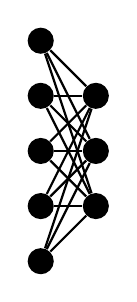
\begin{tikzpicture}[node distance = 0.7 cm]
                                \node (A) [solidNode] {};
                                \node (B) [solidNode, below of = A] {};
                                \node (C) [solidNode, below of = B] {};
                                \node (D) [solidNode, below of = C] {};
                                \node (E) [solidNode, below of = D] {};
                                \node (F) [solidNode, right of = B] {};
                                \node (G) [solidNode, right of = C] {};
                                \node (H) [solidNode, right of = D] {};
                                \draw [link] (A) -- (F);
                                \draw [link] (A) -- (G);
                                \draw [link] (A) -- (H);
                                \draw [link] (B) -- (F);
                                \draw [link] (B) -- (G);
                                \draw [link] (B) -- (H);
                                \draw [link] (C) -- (F);
                                \draw [link] (C) -- (G);
                                \draw [link] (C) -- (H);
                                \draw [link] (D) -- (F);
                                \draw [link] (D) -- (G);
                                \draw [link] (D) -- (H);
                                \draw [link] (E) -- (F);
                                \draw [link] (E) -- (G);
                                \draw [link] (E) -- (H);
                            \end{tikzpicture}
                        \end{figure}
                    \end{example}

                    \begin{theorem}
                        A graph $G$ is bipartite iff every cycle is even.
                    \end{theorem}

                    \begin{proof}
                        ($\Rightarrow$) If the graph $G$ is bipartite, by definition, the vertices of graph can be partition into two groups, that within the group there is no connection between vertices. Therefore, for each cycle, the odd index of vertices and even index of vertices has to be choose alternatively from each groups. Therefore the cycle has to be even.

                        ($\Leftarrow$) Prove by contradiction. A graph can be connected or not connected.

                        If $G$ is connected and has at least two vertices, for an arbitrary vertex $v\in V(G)$, we can calculate the minimum number of edges between the other vertices $v^\prime$ and $v$ (i.e., length, denoted by $l(v^\prime, v)$), for all the vertices that has odd length to $v$, assign them to set $V_1$, for the rest of vertices (and $v$), assign to set $V_2$. Assume that $G$ is not bipartite, which means there are at least one edge between distinct vertices in set $V_1$ or set $V_2$, without lost of generality, assume that edge is $uw$, $u, w\in V_1$. For all vertices in $V_1$ there is an odd length of path between the vertex and $v$, therefore, there exists an odd $l(u,v)$, and an odd $l(w-v)$. The length of cycle $l(u, w, v) = 1 + l(u, v) + l(w, v)$, which is an odd number, it contradict with the prerequisite that all cycles are even, which means the assumption that $G$ is not bipartite is incorrect, $G$ should be bipartite.

                        If $G$ is not connected. Then $G$ can be partition into a set of disjointed subgraphs which are connected with at least two vertices or contains only one vertex. For the component that has more that one vertices, we already proved that it has to be bipartite. For the subgraph $G_i \subset G, i = 1, 2, ..., n$, the vertices can be partition into $V_{i1} \in V(G_i)$ and $V_{i2} \in V(G_i)$, where $V_{i1} \cap V_{i2} = \emptyset$, the union of those subgraphs are bipartite too because $V_1 = \cup_{i=1}^n V_{i1} \in V(G)$ and $V_2 = \cup_{i=1}^n V_{i2} \in V(G)$ satisfied the condition of bipartite. For the subgraph that has one one vertices, those vertices can be assigned into either $V_1$ or $V_2$.
                    \end{proof}

                    \begin{example}
                        The following graph is bipartite, it only contains even cycles.
                        \begin{figure}[H]
                            \centering
                            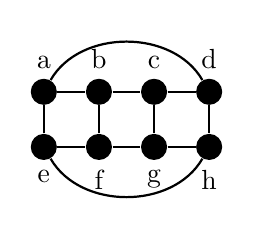
\begin{tikzpicture}[node distance=0.7 cm]
                                \node (a) [solidNode, label=above:{a}] {};
                                \node (b) [solidNode, label=above:{b}, right of = a] {};
                                \node (c) [solidNode, label=above:{c}, right of = b] {};
                                \node (d) [solidNode, label=above:{d}, right of = c] {};
                                \node (e) [solidNode, label=below:{e}, below of = a] {};
                                \node (f) [solidNode, label=below:{f}, below of = b] {};
                                \node (g) [solidNode, label=below:{g}, below of = c] {};
                                \node (h) [solidNode, label=below:{h}, below of = d] {};
                                \draw [link] (a) -- (b);
                                \draw [link] (b) -- (c);
                                \draw [link] (c) -- (d);
                                \draw [link] (a) -- (e);
                                \draw [link] (b) -- (f);
                                \draw [link] (c) -- (g);
                                \draw [link] (d) -- (h);
                                \draw [link] (e) -- (f);
                                \draw [link] (f) -- (g);
                                \draw [link] (g) -- (h);
                                \draw [link] (a) to [out = 60, in = 120, looseness = 1] (d);
                                \draw [link] (e) to [out = 300, in = 240, looseness = 1] (h);
                            \end{tikzpicture}
                        \end{figure}
                        We can rearrange the graph to be more clear as following\\
                        \begin{figure}[H]
                            \centering
                            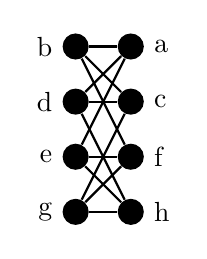
\begin{tikzpicture}[node distance=0.7 cm]
                                \node (a) [solidNode, label=right:{a}] {};
                                \node (b) [solidNode, label=left:{b}, left of=a] {};
                                \node (c) [solidNode, label=right:{c}, below of=a] {};
                                \node (d) [solidNode, label=left:{d}, below of=b] {};
                                \node (e) [solidNode, label=left:{e}, below of=d] {};
                                \node (f) [solidNode, label=right:{f}, below of=c] {};
                                \node (g) [solidNode, label=left:{g}, below of=e] {};
                                \node (h) [solidNode, label=right:{h}, below of=f] {};
                                \draw [link] (a) -- (b);
                                \draw [link] (b) -- (c);
                                \draw [link] (c) -- (d);
                                \draw [link] (a) -- (e);
                                \draw [link] (b) -- (f);
                                \draw [link] (c) -- (g);
                                \draw [link] (d) -- (h);
                                \draw [link] (e) -- (f);
                                \draw [link] (f) -- (g);
                                \draw [link] (g) -- (h);
                                \draw [link] (a) -- (d);
                                \draw [link] (e) -- (h);
                            \end{tikzpicture}
                        \end{figure}
                        The vertices of graph $G$ can be partition into two sets, $\{a, c, f, h\}$ and $\{b, d, e, g\}$
                    \end{example}

                    \begin{example}
                        The following graph is not bipartite

                        \begin{figure}[H]
                            \centering
                            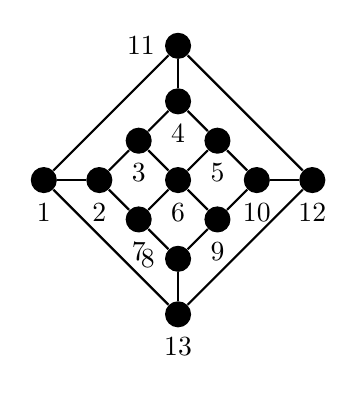
\begin{tikzpicture}[node distance=0.5 cm]
                                \node (11) [solidNode, label=left:{11}] {};
                                \node (4) [solidNode, label=below:{4}, below of=11, yshift=-0.205 cm] {};
                                \node (3) [solidNode, label=below:{3}, below of=4, xshift=-0.5 cm] {};
                                \node (5) [solidNode, label=below:{5}, below of=4, xshift=0.5 cm] {};
                                \node (1) [solidNode, label=below:{1}, below of=3, xshift=-1.205 cm] {};
                                \node (2) [solidNode, label=below:{2}, below of=3, xshift=-0.5 cm] {};
                                \node (6) [solidNode, label=below:{6}, below of=3, xshift=0.5 cm] {};
                                \node (10) [solidNode, label=below:{10}, below of=5, xshift=0.5 cm] {};
                                \node (12) [solidNode, label=below:{12}, below of=5, xshift=1.205 cm] {};
                                \node (7) [solidNode, label=below:{7}, below of=2, xshift=0.5 cm] {};
                                \node (8) [solidNode, label=left:{8}, below of=7, xshift=0.5 cm] {};
                                \node (9) [solidNode, label=below:{9}, below of=6, xshift=0.5 cm] {};
                                \node (13) [solidNode, label=below:{13}, below of=8, yshift=-0.205 cm] {};
                                \draw [link] (11) -- (1);
                                \draw [link] (11) -- (12);
                                \draw [link] (11) -- (4);
                                \draw [link] (4) -- (3);
                                \draw [link] (4) -- (5);
                                \draw [link] (3) -- (2);
                                \draw [link] (3) -- (6);
                                \draw [link] (5) -- (6);
                                \draw [link] (5) -- (10);
                                \draw [link] (1) -- (2);
                                \draw [link] (10) -- (12);
                                \draw [link] (2) -- (7);
                                \draw [link] (6) -- (7);
                                \draw [link] (6) -- (9);
                                \draw [link] (10) -- (9);
                                \draw [link] (7) -- (8);
                                \draw [link] (9) -- (8);
                                \draw [link] (8) -- (13);
                                \draw [link] (1) -- (13);
                                \draw [link] (12) -- (13);
                            \end{tikzpicture}
                        \end{figure}
                        The cycle $c=v_1v_{11}v_4v_3v_2$ have odd number of vertices.
                    \end{example}

            \subsection{Walk, Path and Cycle}
                \paragraph{Walk, trail, path}
                    \begin{definition}[walk]
                        A \textbf{walk} in a graph $G$ is a finite sequence $w=v_0e_1v_1e_2...e_kv_k$, where for each $e_i=v_{i-1}v_i$ the edge and its ends exists in $G$. We say that walk $v_0$ to $v_k$ on $(v_0, v_k)$-walk.
                    \end{definition}

                    \begin{example}
                        \begin{equation*}
                            w = v_2e_4v_3e_4v_2e_5v_3
                        \end{equation*}
                        is a walk, or $(v_2, v_3)$-walk
                    \end{example}

                    \begin{definition}[origin, terminal, internal, length]
                        For $(v_0, v_k)$-walk, The vertices $v_0$ and $v_k$ are called the \textbf{origin} and the \textbf{terminal} of the walk w, $v_1..v_{k-1}$ are called \textbf{internal} vertices. The integer $k$ is the \textbf{length} of the walk. Length of $w$ equals to the number of edges.
                    \end{definition}

                    We can create a reverse walk $w^{-1}$ by reversing $w$.
                    \begin{equation*}
                        w^{-1} = v_ke_kv_{k-1}e_{k-1}...e_2v_1
                    \end{equation*}
                    (The reverse walk is guaranteed to exist because it is an undirected graph)

                    Given two walks $w$ and $w'$ we can create a third walk denoted by $ww'$ by concatenating $w$ and $w'$. The new walk's origin is the same as terminal.

                    \begin{definition}[trail]
                        A \textbf{trail} is a walk with no repeating edges. e.g., $v_3e_4v_2e_5v_3$
                    \end{definition}

                    \begin{definition}[path]
                        A \textbf{path} is a trail with no repeating vertices. e.g., $v_3e_4v_2$
                    \end{definition}

                    Paths $\subseteq$ Trails $\subseteq$ Walks

                \paragraph{Cycle}
                    \begin{definition}[closed, cycle]
                        A path is \textbf{closed} if it has positive length and its origin and terminal are the same. e.g., $v_1e_2v_2e_4v_3e_3v_1$. A closed trail where origin and internal vertices are distinct is called a \textbf{cycle} (The only time a vertex is repeated is the origin and terminal)
                    \end{definition}

                    \begin{definition}[even cycle, odd cycle]
                        A cycle is \textbf{even} if it has a even number of edges otherwise it is \textbf{odd}.
                    \end{definition}

                    \begin{problem}
                        Prove that if $C_1$ and $C_2$ are cycles of a graph, then there exists cycles $K_1, K_2, ..., K_m$ such that $E(C_1)\Delta E(C_2) = E(K_1)\cup E(K_2) \cup...\cup E(K_m)$ and $E(K_i)\cap E(K_j)=\emptyset, \forall i \neq j$. (For set $X$ and $Y$, $X\Delta Y = (X-Y)\cup(Y-X)$, and is called the symmetric difference of $X$ and $Y$)
                    \end{problem}

                    \begin{proof}
                        Proof by constructing $K_1, K_2, ... K_m$. Denote 
                        \begin{align*}
                            C_1 & = v_{11}e_{11}v_{12}e_{12}v_{13}e_{13}...v_{1n}e_{1n}v_{11}\\
                            C_2 & = v_{21}e_{21}v_{22}e_{22}v_{23}e_{23}...v_{2k}e_{2k}v_{21}
                        \end{align*}
                        Assume both cycle start at the same vertice, $v_{11} = v_{12}$. (If there is no intersected vertex for $C_1$ and $C_2$, just simply set $K_1 = C_1$ and $K_2 = C_2$)\\
                        The following algorithm can give us all $K_j, j=1, 2, ... , m$ by constructing $E(C_1)\Delta E(C_2)$.  Also, the complexity is $O(mn)$, which makes the proof doable.\\
                        \begin{algorithm}[H]
                            \caption{Find $K_1, K_2, ... K_m$ by constructing $E(C_1)\Delta E(C_2)$}
                            \begin{algorithmic}[1]
                                \Require Graph $G$, cycle $C_1$ and $C_2$
                                \Ensure $K_1, K_2, ... K_m$
                                \State Initial, $K \gets \emptyset$, $j = 1$
                                \State Set temporary storage units, $v_o \gets v_{11}$, $v_t \gets \emptyset$
                                \For {$i = 1, 2, ..., n$}
                                    \If {$e_{1i} \in C_2$}
                                        \If {$v_o \ne v_{1i}$}
                                            \State $v_t \gets v_{1i}$
                                            \State concatenate $(v_o, v_t)$-path $\subset C_1$ and $(v_o, v_t)$-path $\subset C_2$ to create a new $K_j$
                                            \State Append $K$ with $K_j$, $K \gets K \cup K_j$
                                            \State Reset temporary storage unit. $v_o \gets v_{1(i+1)}$ (or $v_{11}$ if $i = n$), $v_t \gets \emptyset$
                                        \Else
                                            \State $v_o \gets v_{1(i+1)}$ (or $v_{11}$ if $i = n$)
                                        \EndIf
                                    \EndIf
                                \EndFor
                            \end{algorithmic}
                        \end{algorithm}
                        Now we prove that $K_i\cap K_j = \emptyset, \forall i \ne j$. For each $K_j$, it is defined by two $(v_o, v_t)$-paths in the algorithm. From the algorithm we know that all the edges in $(v_o, v_t)$-path in $C_1$ are not intersecting with $C_2$, because if the edge in $C_1$ is intersected with $C_2$, either we closed the cycle $K_j$ before the edge, or we updated $v_o$ after the edge (start a new $K_j$ after that edge). By definition of cycle, all the $(v_o, v_t)$-path that are subset of $C_1$ are not intersecting with each other, as well as all the $(v_o, v_t)$-path that are subset of $C_2$. Therefore, $K_i\cap K_j = \emptyset, \forall i \ne j$.
                    \end{proof}

            \subsection{Some warm-up algorithms}
                \paragraph{Component}
                    \begin{definition}[connected vertices]
                        Two vertices $u$ and $v$ in a graph are said to be \textbf{connected} if there is a path between $u$ and $v$.
                    \end{definition}

                    \begin{definition}[component]
                        Connectivity between vertices is an equivalence relation on $V(G)$, if $V_1, ... V_k$ are the corresponding equivalent classes then $G[V_1]...G[V_k]$ are \textbf{components} of G. If graph has only one component, then we say the graph is connected. A graph is connected iff every pair of vertices in G are connected, i.e., there exists a path between every pair of vertices.
                    \end{definition}

                    The following algorithm finds components in a given graph $G = (V, E)$.

                    \begin{algorithm}[H]
                        \centering
                        \caption{Find components}
                        \begin{algorithmic}[1]
                            \State Let $Q$ be the set of components
                            \For {$i \in V$}
                                \State $Q \gets \{i\}$
                            \EndFor
                            \For {$e = (i, j) \in E$}
                                \For {$p \in Q$}
                                    \For {$q \in Q$}
                                        \If {$i \in p$ and $j \in q$}
                                            \State $Q \gets Q \setminus p \setminus q \cup (p \cup Q)$
                                        \EndIf
                                    \EndFor
                                \EndFor
                            \EndFor
                            \State \Return Q
                        \end{algorithmic}
                    \end{algorithm}

                    We will revisit this procedure when we discuss the subtour elimination constraints for TSP. Such procedure can be improved by introducing disjoint-set forest.

                \paragraph{Cycle detection}
                    The following algorithm is for connected graph, if the graph is not connected, run the algorithm for each component until cycle is detected or all the components have been calculated. Since the complexity for running in connected graph is $O(n + m)$, $n$ as the number of vertices/nodes, and $m$ as the number of edges/arcs, the running time of disconnected graph is the \textbf{summation} of running time in each component, where each component is connected. Therefore the complexity is the same in disconnected graph as in connected graph.

                    The main idea is starting with arbitrary vertex/node, using DFS or BFS to search on the graph try to revisit the vertex/node we start with. If succeed, a cycle is detected, otherwise if all the vertices/nodes has been visited, then no cycle exists. And in linked-list representation, the complexity is $O(|V| + |E|)$, i.e. $O(n + m)$. However, there is slightly different in undirected graph and directed graph, for undirected graph needs at least three vertices to form a cycle while directed graph needs at least two.

                    Here is the detail algorithm (DFS) for undirected graph:
                    \begin{algorithm}[H]
                        \caption{Main algorithm}
                        \begin{algorithmic}[1]
                            \State For all nodes, labeled as ``unvisited''
                            \State Arbitrary choose a vertex $v$, add a dummy vertex $w$, add a dummy edge $(w, v)$, label $w$ as ``visited''
                            \State run $DFS(w, v)$
                            \State Remove dummy vertex $w$ and dummy edge $(w, v)$
                            \If {$DFS(w, v)$ returns ``Cycle is found''}
                                \State \Return ``Cycle is found''
                            \Else
                                \State \Return ``No cycle detected''
                            \EndIf
                        \end{algorithmic}
                    \end{algorithm}

                    \begin{algorithm}[H]
                        \caption{DFS(w, v)}
                        \begin{algorithmic}[1]
                            \State Label $v$ as ``visited''
                            \If {number of $v$ 's neighbor is 1}
                                \State \Return null
                            \Else
                                \For {all neighbor $u$ in linked-list of $v$ excepts $w$}
                                    \If {$u$ is labeled as ``visited''} 
                                        \State \Return ``Cycle is found'' 
                                    \Else
                                        \State run $DFS(v, u)$
                                    \EndIf
                                \EndFor
                            \EndIf
                        \end{algorithmic}
                    \end{algorithm}

                    Now check the complexity. Denote $v\in N$ as a node in graph $G$, total number of nodes denoted by $n$, denote $d_v$ as number of neighbors of node $v$. The complexity of $DFS(w, v)$ is $O(d_v)$ for each node $v$ it visited (it should be $O(v)$ because we need $O(1)$ to check if a node is $w$), each node can only be visited, by ``visited'' it means $DFS(w, v)$ is executed, at most once, which is controlled by the ``visited'' label. The total complexity is $O(n + \sum_{v\in N} d_v) = O(n + m)$

                \paragraph{Test Bipartiteness}
                    We have proved that a bipartite graph only has even cycles, and the graph with only even cycles are bipartite graph, however, that is not very convenient to test if a graph is bipartite because it needs to enumerate all cycles.

                    The other idea to test bipartiteness is try to color the vertices of the graph, if it can be 2-colored, then the graph is bipartite, otherwise it is not.

                    The following is the algorithm (using BFS)
                    \begin{algorithm}[H]
                        \caption{Test Bipartiteness}
                        \begin{algorithmic}[1]
                            \State Initialize, $head \gets 1$, $tail \gets 1$, $queue[1] \gets s$, mark all vertices as ``unvisited''
                            \State Mark $s$ as ``visited''
                            \State $color[s] \gets 0$
                            \While {$head \ge tail$}
                                \State $v \gets queue[tail]$, $tail \gets tail + 1$
                                \For {$\forall u \in d_v$}
                                    \If {$u$ is ``unvisited''}
                                        \State $head \gets head + 1$, $queue[head] = u$
                                        \State Mark $u$ as ``visited''
                                        \State $color[u] \gets 1 - color[v]$
                                    \Else
                                        \If {$color[u] == color[v]$}
                                            \Return False
                                        \EndIf
                                    \EndIf
                                \EndFor
                            \EndWhile
                            \Return True
                        \end{algorithmic}
                    \end{algorithm}

                \paragraph{Bridge}
                    \begin{definition}[Tree Edge, Cross Edge, Vertical Edge]
                        Given a graph $G = (V, E)$ and a rooted tree $T$ in $G$, edge in $G$ can be classified by three types:
                        \begin{itemize}
                            \item Tree edges: edge in $T$
                            \item Cross edges: $(u, v)$, $u$ and $v$ do not have an ancestor-descendant relation
                            \item Vertical edges: $(u, v)$, $u$ is an ancestor of $v$, or $v$ is an ancestor of $u$
                        \end{itemize}

                        \begin{figure}[H]
                            \centering
                            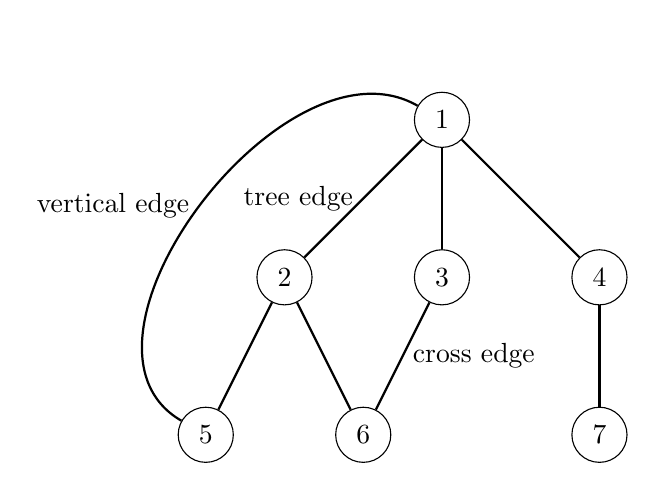
\begin{tikzpicture}[node distance=2 cm]
                                \node (1) [circleNode] {1};
                                \node (2) [circleNode, below of=1, xshift = -2 cm] {2};
                                \node (3) [circleNode, below of=1] {3};
                                \node (4) [circleNode, below of=1, xshift = 2 cm] {4};
                                \node (5) [circleNode, below of=2, xshift = -1 cm] {5};
                                \node (6) [circleNode, below of=2, xshift = 1 cm] {6};
                                \node (7) [circleNode, below of=4] {7};
                                \draw [link] (1) -- node [left] {tree edge} (2);
                                \draw [link] (1) -- (3);
                                \draw [link] (1) -- (4);
                                \draw [link] (2) -- (5);
                                \draw [link] (2) -- (6);
                                \draw [link] (4) -- (7);
                                \draw [link] (3) -- node [right] {cross edge} (6);
                                \draw [link] (1) to [out = 150, in = 150] node [left] {vertical edge} (5);
                            \end{tikzpicture}
                        \end{figure}
                    \end{definition}

                    In a BFS tree $T$ of a graph $G$, there can not be vertical edges, there cannot be cross edges $(u, v)$ with $u$ and $v$ 2 levels apart. (Cross edge at most 1 level apart)

                    In a DFS tree $T$ of a graph $G$, there can not be cross edges, there can only be tree edges and vertical edges.

                    \begin{definition}[bridge]
                        Given a connected graph $G=(V, E)$, an edge $e \in E$ is called a \textbf{bridge} if the graph $G=(V, E\setminus \{e\})$ is disconnected.
                    \end{definition}

                    The idea to find bridge is through a DFS tree. Notice that there are only tree edges and vertical edges in DFS tree. Vertical edges are not bridges, a tree edge $(u, v)$ is not a bridge if some vertical edge jumping from below $u$ to above $v$. Other tree edges are bridges.

                    Define $level(v)$ as the level of vertex $v$ in DFS tree. $T_v$ as the sub tree rooted at $v$, $h(v)$ as the smallest level that can be reached using a vertical edge from vertices in $T_v$. $(parent(u), u)$ is a bridge if $h(u) \ge level(u)$. The algorithm is as following:
                    \begin{algorithm}[H]
                        \caption{FindBridge(G)}
                        \begin{algorithmic}[1]
                            \State Mark all vertices as ``unvisited''
                            \For {$v \in V$}
                                \If {$v$ is ``unvisited''}
                                    \State $level(v) \gets 0$
                                    \State \texttt{RecursiveDFS(v)}
                                \EndIf
                            \EndFor
                        \end{algorithmic}
                    \end{algorithm}

                    \begin{algorithm}[H]
                        \caption{RecursiveDFS(v)}
                        \begin{algorithmic}[1]
                            \State mark $v$ as ``visited''
                            \State $h(v) \gets \infty$
                            \For {$u \in d_v$}
                                \If {$u$ is ``unvisited''}
                                    \State $level(u) \gets level(v) + 1$
                                    \State \texttt{RecursiveDFS(u)}
                                    \If {$h(u) \ge level(u)$}
                                        \State $(u, v)$ is a bridge
                                    \EndIf
                                    \If {$h(u) < h(v)$}
                                        \State $h(v) \gets h(u)$
                                    \EndIf
                                \Else
                                    \If {$level(u) < level(v) - 1$ and $level(u) < h(v)$}
                                        \State $h(v) \gets level(u)$
                                    \EndIf
                                \EndIf
                            \EndFor
                        \end{algorithmic}
                    \end{algorithm}

        \section{Matching}
            \subsection{Matching}
                \begin{definition}[matching, M-saturated, M-unsaturated]
                    Let $G = (V, E)$ be a graph, a \textbf{matching} is a subset of edges $M \subseteq E$ such that no two elements of $M$ are adjacent. The two ends of an edge in $M$ are said to be \textbf{matched} under $M$. A matching $M$ saturates a vertex $v$, and $v$ is said to be \textbf{M-saturated}, if some edge of $M$ is incident with $v$. Otherwise, $v$ is \textbf{M-unsaturated}.
                \end{definition}

                \begin{definition}[perfect matching, maximum matching]
                    If every vertex of $G$ is M-saturated, then the matching is said to be \textbf{perfect matching}, for perfect matching, we have $|M| = \frac{|V(G)|}{2}$. $M$ is a \textbf{maximum matching} if $G$ has no matching $M^\prime$ with $|M^\prime| > |M|$. Every perfect matching is maximum. The maximum matching does not necessarily to be perfect. Perfect matching and maximum matching may not be unique.
                \end{definition}

                \begin{definition}[M-alternating]
                    An \textbf{M-alternating} path in $G$ is a path whose edges are alternately in $E\setminus M$ and $M$.
                \end{definition}

                \begin{definition}[M-augmenting]
                    An \textbf{M-augmenting} path in $G$ is an $M$-alternating path whose origin and terminus are $M$-unsaturated.
                \end{definition}

                \begin{lemma}
                    Every augmenting path $P$ has property that let $M^\prime = P\Delta M = (M \cup P) \setminus (M \cap P)$ then $M^\prime$ contains one more edge then $M$
                \end{lemma}

                The following path is an $M$-augmenting path
                \begin{figure}[H]
                    \centering
                    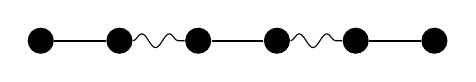
\begin{tikzpicture}
                        \node (0) [solidNode] {};
                        \node (1) [solidNode, right of=0] {};
                        \node (2) [solidNode, right of=1] {};
                        \node (3) [solidNode, right of=2] {};
                        \node (4) [solidNode, right of=3] {};
                        \node (5) [solidNode, right of=4] {};
                        \draw (0) [link] -- (1);
                        \draw (1) [matchedLink] -- (2);
                        \draw (2) [link] -- (3);
                        \draw (3) [matchedLink] -- (4);
                        \draw (4) [link] -- (5);
                    \end{tikzpicture}
                \end{figure}

                The following path is $M^\prime = P\Delta M (M \cup P) \setminus (M \cap P)$ and all the vertices are $M$-saturated.

                \begin{figure}[H]
                    \centering
                    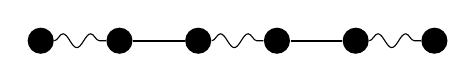
\begin{tikzpicture}
                        \node (0) [solidNode] {};
                        \node (1) [solidNode, right of=0] {};
                        \node (2) [solidNode, right of=1] {};
                        \node (3) [solidNode, right of=2] {};
                        \node (4) [solidNode, right of=3] {};
                        \node (5) [solidNode, right of=4] {};
                        \draw (0) [matchedLink] -- (1);
                        \draw (1) [link] -- (2);
                        \draw (2) [matchedLink] -- (3);
                        \draw (3) [link] -- (4);
                        \draw (4) [matchedLink] -- (5);
                    \end{tikzpicture}
                \end{figure}

                \begin{theorem}[Berge, 1957]
                    A matching $M$ in a graph $G$ is maximum iff $G$ has no M-augmenting path.
                \end{theorem}

                \begin{proof}
                    ($\Rightarrow$) It is clear that if $M$ is maximum, it has no augmenting paths since otherwise by problem claim we can increase by one.

                    ($\Leftarrow$) Suppose $M$ is not maximum and let $M^\prime$ be a bigger matching. Let $A = M \Delta M^\prime$ now no vertex of $G$ is incident to more than two members of $A$. For otherwise either two members of $M$ or two members of $M^\prime$ would be adjacent. Contradict the definition of matching. It follows that every component of the edges incident subgraph $G[A]$ is either an even cycle with edge augmenting in $M\Delta M^\prime$ or else $A$ path with edges alternating between $M$ and $M^\prime$.

                    Since $|M^\prime| \ge |M|$ then the even cycle cannot help because exchanging $M$ and $M^\prime$ will have same cardinality.

                    The path case implies that $p$ is alternating in $M$ and since $|M^\prime| > |M|$ the end arc exposed so that $p$ is augmenting.
                \end{proof}

                \begin{definition}[Vertex-cover]
                    The \textbf{vertex-cover} is a subset of vertices $X$ such that every edge of $G$ is incident to some member of $X$.
                \end{definition}

                \begin{lemma}
                    The cardinality of any matching is less than or equal to the cardinality of any vertex cover.
                \end{lemma}

                \begin{proof}
                    Consider any matching. Any vertex cover must have nodes that at least incident to the edges in the matching. Since all the edges in the matching are disjointed, so for a single node can at most cover one edge in the matching. If the matching is not perfect, for the edges that not in the tree, they may or may not be possible to be covered by the nodes incident to the edges in the matching, with an easy triangle graph example, we can prove this lemma.
                \end{proof}

                \begin{theorem}[K\"onig Theorem]
                    If $G$ is bipartite, the cardinality of the maximum matching is equal to the cardinality of the minimum vertex cover.
                \end{theorem}

                \begin{proof}
                    Let $G$ be a bipartite graph, $G = (V, E)$ where $V = X\cup Y$ as $X$ and $Y$ are two disjointed sets of vertices. Let $M$ be a maximum matching on $G$. For each edge in $M$, denoted by $e_i = a_ib_i$ where $e_i \in M$, $a_i \in A$ and $b_i \in B$ and $A = \{a_i: e_i \in M\} \subseteq X$, and $B = \{b_i: e_i \in M\} \subseteq Y$. Therefore, we can partition $X$ by $A$ and $U = X\setminus A$, partition $Y$ by $B$ and $W = Y\setminus B$.

                    We can further partition the matching $M$ into $M_1$ and $M_2$. For all the edges in $M_1$ can be included into an $M$-alternating path starts from a vertex in $U$ (which includes the edges directly linked to vertices in $U$), and $M_2 = M \setminus M_1$. For edges in $M_1$, we take the ends of edges in $B$ in the vertex cover, denoted by $B_1$, take the ends of edges in $A$ as a subset denoted by $A_1 \subseteq A$. For the edges in $M_2$, we take the ends of edges in $A$ in the vertex cover, denoted by $A_2$, and the ends of edges in $B$ as a subset denoted by $B_2 \subseteq B$. 

                    We claim that all the vertices in $U$ can only be connected to vertices in $B_1$ and vertices in $W$ can only be connected to vertices in $A_2$.

                    $U \subset X$ connects to vertices in $B_1$ by definition. If vertices in $W \subset Y$ is connected to vertices in $A_1$, then we will have $M$-augmenting path which is contradicted to the assumption that $M$ is maximum matching.
                \end{proof}

                The following is an example. Where the edge in the matching that accessible from members of $U = \{1, 2\}$ in an $M$-alternating path is edge $3a, 4b, 5c, 6d$.

                \begin{figure}[H]
                    \centering
                    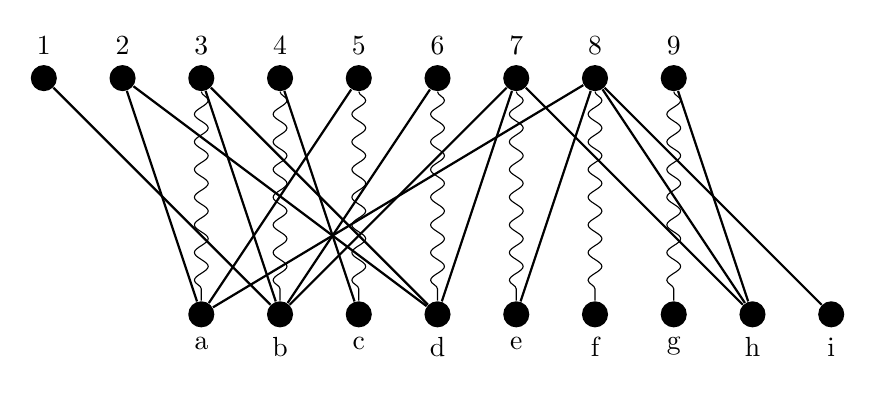
\begin{tikzpicture}
                        \node (1) [solidNode, label=above:{1}] {};
                        \node (2) [solidNode, right of = 1, label=above:{2}] {};
                        \node (3) [solidNode, right of = 2, label=above:{3}] {};
                        \node (4) [solidNode, right of = 3, label=above:{4}] {};
                        \node (5) [solidNode, right of = 4, label=above:{5}] {};
                        \node (6) [solidNode, right of = 5, label=above:{6}] {};
                        \node (7) [solidNode, right of = 6, label=above:{7}] {};
                        \node (8) [solidNode, right of = 7, label=above:{8}] {};
                        \node (9) [solidNode, right of = 8, label=above:{9}] {};
                        \node (a) [solidNode, below of = 3, yshift=-2 cm, label=below:{a}] {};
                        \node (b) [solidNode, right of = a, label=below:{b}] {};
                        \node (c) [solidNode, right of = b, label=below:{c}] {};
                        \node (d) [solidNode, right of = c, label=below:{d}] {};
                        \node (e) [solidNode, right of = d, label=below:{e}] {};
                        \node (f) [solidNode, right of = e, label=below:{f}] {};
                        \node (g) [solidNode, right of = f, label=below:{g}] {};
                        \node (h) [solidNode, right of = g, label=below:{h}] {};
                        \node (i) [solidNode, right of = h, label=below:{i}] {};
                        \draw [matchedLink] (3) -- (a);
                        \draw [matchedLink] (4) -- (b);
                        \draw [matchedLink] (5) -- (c);
                        \draw [matchedLink] (6) -- (d);
                        \draw [matchedLink] (7) -- (e);
                        \draw [matchedLink] (8) -- (f);
                        \draw [matchedLink] (9) -- (g);
                        \draw [link] (1) -- (b);
                        \draw [link] (2) -- (a);
                        \draw [link] (8) -- (i);
                        \draw [link] (8) -- (h);
                        \draw [link] (3) -- (b);
                        \draw [link] (3) -- (d);
                        \draw [link] (2) -- (d);
                        \draw [link] (4) -- (c);
                        \draw [link] (5) -- (a);
                        \draw [link] (6) -- (b);
                        \draw [link] (7) -- (b);
                        \draw [link] (7) -- (d);
                        \draw [link] (7) -- (h);
                        \draw [link] (8) -- (e);
                        \draw [link] (8) -- (a);
                        \draw [link] (9) -- (h);
                    \end{tikzpicture}
                \end{figure}

                In which $U = \{1, 2\}$, $M_1 = \{3a, 4b, 5c, 6d\}$. $U = \{1, 2,\}, A_1 = \{3, 4, 5, 6\}, A_2 = \{7, 8, 9\}, W=\{h, i\}, B_1 = \{a, b, c, d\}, B_2 = \{e, f, g\}$. The vertex cover is $\{a, b, c, d, 7, 8, 9\}$.

                The above theorem does not apply to non-bipartite graph. The following is an example
                \begin{figure}[H]
                    \centering
                    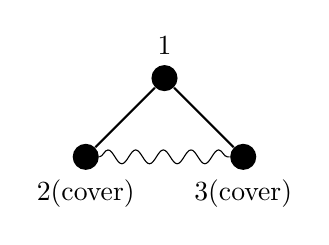
\begin{tikzpicture}
                        \node (1) [solidNode, label=above:{1}] {};
                        \node (2) [solidNode, below of = 1, xshift = -1 cm, label=below:{2(cover)}] {};
                        \node (3) [solidNode, below of = 1, xshift = 1 cm, label=below:{3(cover)}] {};
                        \draw [matchedLink] (2) -- (3);
                        \draw [link] (1) -- (2);
                        \draw [link] (1) -- (3);
                    \end{tikzpicture}
                \end{figure}

                The maximum matching has one edge, where the minimum cover has two vertices.

            \subsection{Blossom Algorithm}
                First, for the bipartite graphs, there is no odd cycles in the graph, the maximum matching can be derived by repeatedly extend the existing augmenting paths. For the non-bipartite algorithm, we use the Blossom algorithm to find maximum matching.

                \paragraph{Blossom}
                A blossom is a set of nodes and edges starting at an unsaturated vertex, with a stem of even number of edges, and link to an odd cycle of edges. 

                \begin{figure}[H]
                    \centering
                    \includegraphics[width=0.4\textwidth]{"../../image/blossom"}
                    \caption{An example of blossom}
                \end{figure}

                \paragraph{Pseudo codes}
                    \begin{algorithm}
                        \centering
                        \caption{Blossom algorithm}
                        \begin{algorithmic}
                            \State Let $F$ be the set of unsaturated nodes
                            \While {$F \neq \emptyset$}
                                \State Let $r \in F$ be an unsaturated node
                                \State queue.push($r$)
                                \State $T \gets \emptyset$
                                \State $T$.add($r$)
                                \While {queue $\neq \emptyset$}
                                    \State $v \gets$ queue.pop()
                                    \For {All neighbor $w$ of $v$}
                                        \If {$w \notin T$ and $w$ is saturated}
                                            \State $T$.add(w)
                                            \State $T$.add(mate(w)), mate(w) is another neighbor of $w$
                                            \State queue.push(mate(w))
                                        \ElsIf {$w \in T$ and odd cycle detected}
                                            \State Contract cycle
                                        \ElsIf {$w \in F$}
                                            \State Expand all contract cycles
                                            \State Reconstruct augmenting path
                                            \State Augment path by inverting edges
                                        \EndIf
                                    \EndFor
                                \EndWhile
                            \EndWhile
                        \end{algorithmic}
                    \end{algorithm}    

        \section{Maximum Flow Problem}
            \subsection{Maximum Flow Problem}
                Let $D=(V, A)$ be a strict digraph with distinguished vertices $s$ and $t$. We call $s$ the source and $t$ the sink, let $u=\{u_e: e\in A\}$ be a nonnegative integer-valued capacity function defined on the arcs of $D$. The maximum flow problem on $(D, s, t, u)$ is the following Linear program.
                \begin{align*}
                    \max \quad & v\\
                    \text{s.t.} \quad & \sum_{h(e)=i}x_e - \sum_{t(e) = i} x_e = \begin{cases}
                        -v, \quad \text{if } i = s\\
                        v, \quad \text{if } i = t \\
                        0, \quad \text{otherwise}
                    \end{cases}\\
                    & 0\le x_e \le u_e, \quad \forall e\in A
                \end{align*}
                We think of $x_e$ as being the flow on arc $e$. Constraint says that for $i \neq s, t$ the flow into a vertex has to be equal to the flow out of vertex. That is, flow is conceded at vertex $i$ for $i=s$ and for $i=t$ the net flow in the entire digraph must be equal to $v$. A $\mathbf{x_e}$ that satisfied the above constraints is an $(s,t)$-flow of value $v$. If in addition it satisfies the bounding constraints, then it is a feasible $(s,t)$-flow. A feasible $(s,t)$-flow that has maximum $v$ is optimal on maximum.

                \begin{theorem}
                    For $S \subseteq V$ we define $(S, \bar{S})$ to be a $(s, t)$-cut if $s\in S$ and $t\in \bar{S}=V-S$, the capacity of the cut, denoted $u(S, \bar{S})$ as $\sum \{u_e: e\in \delta^-(S)\}$ where $\delta^-(S) = \{e\in A: t(e) \in S \text{ and } h(e) \in \bar{S}\}$
                \end{theorem}

                \begin{example}
                    For the following graph:
                    \begin{figure}[H]
                        \centering
                        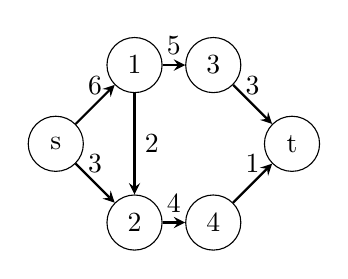
\begin{tikzpicture}[node distance = 1 cm]
                            \node (1) [circleNode] {1};
                            \node (3) [circleNode, right of=1] {3};
                            \node (s) [circleNode, below of=1, xshift = -1 cm] {s};
                            \node (2) [circleNode, below of=s, xshift = 1 cm] {2};
                            \node (t) [circleNode, below of=3, xshift = 1 cm] {t};
                            \node (4) [circleNode, below of=t, xshift = -1 cm] {4};
                            \draw [arrow] (s) -- node [above] {6} (1);
                            \draw [arrow] (s) -- node [above] {3} (2);
                            \draw [arrow] (1) -- node [right] {2} (2);
                            \draw [arrow] (1) -- node [above] {5} (3);
                            \draw [arrow] (2) -- node [above] {4} (4);
                            \draw [arrow] (3) -- node [above] {3} (t);
                            \draw [arrow] (4) -- node [above] {1} (t);
                        \end{tikzpicture}
                    \end{figure}
                    Let $S = \{1, 2, 3, s\}$, $\bar{S} = \{4, t\}$\\
                    then $\delta^-(S) = \{(2, 4), (3, t)\} \Rightarrow u(S, \bar{S}) = 7$
                \end{example}

                \begin{definition}
                    If $(S, \bar{S})$ has minimum capacity of all $(s,t)$-cuts, then it is called \textbf{minimum cut}.
                \end{definition}

                \begin{definition}
                    Let $\delta^+(S) = \delta^-(V-S)$
                \end{definition}

                \begin{example}
                    \begin{figure}[H]
                        \centering
                        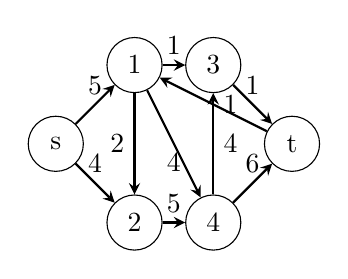
\begin{tikzpicture}[node distance = 1 cm]
                            \node (1) [circleNode] {1};
                            \node (3) [circleNode, right of=1] {3};
                            \node (s) [circleNode, below of=1, xshift = -1 cm] {s};
                            \node (2) [circleNode, below of=s, xshift = 1 cm] {2};
                            \node (t) [circleNode, below of=3, xshift = 1 cm] {t};
                            \node (4) [circleNode, below of=t, xshift = -1 cm] {4};
                            \draw [arrow] (s) -- node [above] {5} (1);
                            \draw [arrow] (s) -- node [above] {4} (2);
                            \draw [arrow] (1) -- node [left] {2} (2);
                            \draw [arrow] (1) -- node [above] {1} (3);
                            \draw [arrow] (1) -- node [below] {4} (4);
                            \draw [arrow] (2) -- node [above] {5} (4);
                            \draw [arrow] (4) -- node [right] {4} (3);
                            \draw [arrow] (3) -- node [above] {1} (t);
                            \draw [arrow] (4) -- node [above] {6} (t);
                            \draw [arrow] (t) -- node [right] {1} (1);
                        \end{tikzpicture}
                    \end{figure}

                    Let $S = \{s, 1, 2, 3\}$, $\bar{S} = \{4, t\}$, $u(S, \bar{S}) = u_{14} + u_{24} + u_{3t} = 10$, $\delta^-(S) = \{(1, 4), (2, 4), (3, t)\}$, $\delta^+(S) = \{(4, 3), (t, 1)\}$
                \end{example}

                \begin{lemma}
                    If $x$ is a $(s, t)$ flow of value $v$ and $(S, \bar{S})$ is a $(s, t)$-cut, then
                    \begin{equation*}
                        v = \sum_{e\in \delta^-(S)} x_e - \sum_{e\in \delta^+(S)} x_e
                    \end{equation*}
                \end{lemma}

                \begin{proof}
                    Summing the first set of constraints over the vertices of $S$,
                    \begin{equation*}
                        \sum_{i\in S} (\sum_{h(e) = i}x_e - \sum_{t(e) = i}x_e) = -v
                    \end{equation*}
                    Now for an arc $e$ with both ends in $S$, $x_e$ will occur twice once with a positive and once with negative so they cancel and the above sum is reduced to
                    \begin{equation*}
                        \sum_{e\in \delta^+(S)}x_e - \sum_{e \in \delta^-(S)}x_e = -v
                    \end{equation*}
                \end{proof}

                Flow is the prime variable, capacity is the dual variable.

                \begin{corollary}
                    If $x$ is a feasible flow of value $v$, and $(S, \bar{S})$ is an $(s, t)$-cut, then
                    \begin{equation*}
                        v \le u(S, \bar{S}) \quad \text{(Weak duality)}
                    \end{equation*}
                \end{corollary}

                \begin{definition}
                    Define an arc $e$ to be \textbf{saturated} if $x_e = u_e$, and to be \textbf{flowless} if $x_e = 0$
                \end{definition}

                \begin{corollary}
                    Let $x$ be a feasible flow and $(S, \bar{S})$ be a $(s, t)$-cut, if $\forall e\in \delta^-(S)$ is saturated, and $\forall e\in \delta^+(S)$ is flowless, then $x$ is a maximum flow and $(S, \bar{S})$ is a minimum cut. (Strong duality)
                \end{corollary}

                \begin{proof}
                    If every arc of $\delta^-(S)$ is saturated then
                    \begin{equation*}
                        \sum_{e\in \delta^-(S)}x_e = \sum_{e\in \delta^-(S)}u_e
                    \end{equation*}
                    If every arc of $\delta^+(S)$ is flowless then
                    \begin{equation*}
                        \sum_{e\in \delta^+(S)}x_e = 0
                    \end{equation*}
                    $\Rightarrow$ $x$ is as large as it can get when as $u(S, \bar{S})$ is as small as it can get.
                \end{proof}

            \subsection{Prime and Dual of Maximum Network Flow Problem}
                The LP of maximum flow can be modeled as following, WLOG, we let $s = v_1 \in V, t = v_{|V|} \in V$.
                \begin{align*}
                    \max \quad & f = \left[\begin{matrix}0 & 0 & \cdots & 0 & 1\end{matrix}\right]\left[\begin{matrix}\mathbf{x} \\ f\end{matrix}\right]\\
                    \text{s.t.} \quad & \left[\begin{matrix}\mathbf{A} & \mathbf{F}\end{matrix}\right]\left[\begin{matrix}\mathbf{x}\\ f\end{matrix}\right] = \mathbf{0}\\
                    & \mathbf{Ix} \le \mathbf{u}\\
                    & \left[\begin{matrix}\mathbf{x}\\ f\end{matrix}\right] \ge 0
                \end{align*}

                In which $\mathbf{A}$ is the vertex-arc incident matrix and $\mathbf{F}$ is a column vector where the first row is -1, last row is 1 and all other rows are 0s, which is because we denote the first vertex as source $s$ and the last vertex as the sink $t$. $\mathbf{u}$ is the column vector of upper bound of each arcs.
                \begin{align*}
                    \mathbf{A} &= \mathbf{A}_{|E|\times |V|} = [a_{ij}], \text{ where } a_{ij} = \begin{cases}
                        1, \quad \text{if $v_i = h(e_j)$} \\
                        -1, \quad \text{if $v_i = t(e_j)$} \\
                        0, \quad \text{otherwise}
                    \end{cases}\\
                    \mathbf{F} &= \left[\begin{matrix}-1 & \cdots & 0 & \cdots & 1\end{matrix}\right]^\top \\
                    \mathbf{u} &= \left[\begin{matrix}u_1 & u_2 & \cdots & u_{|E|}\end{matrix}\right]^\top
                \end{align*}

                Then, we take the dual of LP
                \begin{align*}
                    \min \quad & \mathbf{u}\mathbf{w_E} \\
                    \text{s.t.} \quad & \left[\begin{matrix}
                        \mathbf{w_V} & \mathbf{w_E}
                    \end{matrix}\right]\left[\begin{matrix}
                        \mathbf{A} \\ \mathbf{I}
                    \end{matrix}\right] \ge 0 \\
                    & \left[\begin{matrix}
                        \mathbf{w_V} & \mathbf{w_E}
                    \end{matrix}\right]\left[\begin{matrix}
                        \mathbf{F} \\\mathbf{0}
                    \end{matrix}\right] = 1\\
                    & \mathbf{w_V} \quad \text{unrestricted} \\
                    & \mathbf{w_E} \ge \mathbf{0}
                \end{align*}

                In which $\mathbf{w_V}$ is ``whether or not'' vertex $v$ is in $S$ where $(S, \bar{S})$ represents a cut, $\mathbf{w_E}$ is ``whether or not'' an arc in in $\delta^+(S)$. $\mathbf{u}, \mathbf{E}, \mathbf{F}$ have the same meaning as in prime.
                \begin{align*}
                    \mathbf{w_V} &= \left[\begin{matrix}w_1 & w_2 & \cdots & w_{|V|}\end{matrix}\right]^\top \\
                    \mathbf{w_E} &= \left[\begin{matrix}w_{|V| + 1} & w_{|V| + 2} & \cdots & w_{|V| + |E|}\end{matrix}\right]^\top
                \end{align*}

                To make it more clear, it can be rewritten as following
                \begin{align*}
                    \min \quad & \sum_{e \in E} u_ew_e\\
                    \text{s.t.} \quad & w_i - w_j + w_{|V| + e} \ge 0, \forall e = (i, j) \in E\\
                    & -w_1 + w_{|V|} = 1\\
                    & \mathbf{w_V} \quad \text{unrestricted} \\
                    & \mathbf{w_E} \ge \mathbf{0}
                \end{align*}

                The meaning for the first set of constraint is to decide whether or not an arc is in $\delta^+(S)$ of a $(S, \bar{S})$, which is decided by $w_V$. The $w_1 - w_{|V|} = 1$, which is the second set of constraint means the source $s = v_1$ and the sink $t = v_{|V|}$ has to be in $S$ and $\bar{S}$ respectively.

            \subsection{Maximum Flow Minimum Cut Theorem}
                \begin{definition}
                    Let $P$ be a path, (not necessarily a dipath), $P$ is called \textbf{unsaturated} if every \textbf{forward} arc is unsaturated ($x_e < u_e$) and every \textbf{reverse} arc has positive flow ($x_e > 0$). If in addition $P$ is an $(s, t)$-path, then $P$ is called an \textbf{x-augmenting path}
                \end{definition}

                \begin{theorem}
                    A feasible flow $x$ in a digraph $D$ is maximum iff $D$ has no augmenting paths.
                \end{theorem}

                \begin{proof}
                    (Prove by contradiction) 

                    ($\Rightarrow$) Let $x$ be a maximum flow of value $v$ and suppose $D$ has an augmenting path. Define in $P$ (augmenting path):
                    \begin{align*}
                        & D_1 = \min \{u_e-x_e: e \text{ forward in } P\} \\
                        & D_2 = \min \{x_e: e \text{ backward in } P\}\\
                        & D = \min \{D_1, D_2\}
                    \end{align*}
                    Since $P$ is augmenting, then $D > 0$, let
                    \begin{align*}
                        \hat{x_e} = \begin{cases}
                            x_e + D \quad \text{If $e$ is forward in $P$}\\
                            x_e - D \quad \text{If $e$ is backward in $P$}\\
                            x_e \quad otherwise
                        \end{cases}
                    \end{align*}
                    It is easy to see that $\hat{x}$ is feasible flow and that the value is $V+D$, a contradiction.

                    ($\Leftarrow$) Suppose $D$ admits no x-augmenting path, Let $S$ be the set of vertices reachable from $s$ by x-unsaturated path clearly $s\in S$ and $t\notin S$ (because otherwise there would be an augmenting path). Thus, $(S, \bar{S})$ is a $(s, t)$-cut.

                    Let $e\in \delta^-(S)$ then $e$ must be saturated. For otherwise we could add the $h(e)$ to $S$

                    Let $e\in \delta^+(S)$ then $e$ must be flow less. For otherwise we could add the $t(e)$ to $S$.

                    According to previous corollary, that $x$ is maximum.
                \end{proof}

                \begin{theorem}(Max-flow = Minimum-cut)
                    For any digraph, the value of a maximum $(s, t)$-flow is equal to the capacity of a minimum $(s, t)$-cut
                \end{theorem}

            \subsection{Ford-Fulkerson Method}

                \paragraph{Augmenting path}
                    An augmenting path is a path of edges in the residual graph with unused capacity greater than zero from the source $s$ to target $t$. Every augmenting path has a bottleneck, which limits the flow that can go through this path.

                \paragraph{Ford-Fulkerson method}
                    The Ford-Fulkerson method is a greedy algorithm with the following procedures:

                    \begin{itemize}
                        \item Iteratively find a path $P$ from $s \rightarrow t$ with $c_f(e) = c(e) - f(e)$, where $f$ is the current flow, and $c_f$ is the so called residual capacity where
                        \begin{equation}
                            \forall (u, v) \in E: c_f(u, v) = c(u, v) - f(u, v),\quad \text{if } f(u, v) \ge 0: c_f(v, u) = f(u, v)
                        \end{equation}
                        \item Then, define $\delta(P) = \min_{e \in P} c_f(e)$ and
                        \begin{equation}
                            f_P(e) = \begin{cases}
                                \delta(P), \quad \text{if } e\in P\\0, \quad \text{otherwise}
                            \end{cases}
                        \end{equation}
                        then we assign new values to the flow at each edge
                        \begin{equation}
                            f_{new} = f_{old} + f_P
                        \end{equation}
                        where both flows satisfy noon-negativity, capacity, and flow conservation constraints. And by the definition of the residual capacities, the original capacities constraints are never violated.
                        \item The procedure terminates when no such path $s \rightarrow t$ can be found with $c_f(e) \ge 0$.
                    \end{itemize}
                    
                    The Ford-Fulkerson method

                    \begin{algorithm}
                        \centering
                        \caption{Ford-Fulkerson method}
                        \begin{algorithmic}
                            \State Initialize, set $f(e) = 0, \forall e \in E, G_f = G$
                            \While {$\exists P = s \rightarrow t \in G_f$ such that $\forall e \in E, c_f(e) \ge 0$}
                                \State $\delta(P) = \min_{e \in P} c_f(e)$
                                \For {$\forall (u, v) \in P$}
                                    \If {$f(u, v) > 0$}
                                        \State $f(v, u) = f(v, u) - \delta(P)$
                                    \Else
                                        \State $f(u, v) = f(u, v) + \delta(P)$
                                    \EndIf
                                \EndFor
                                \State Update $G_f$
                            \EndWhile
                        \end{algorithmic}
                    \end{algorithm}

                \paragraph{Some implementations}
                    \begin{itemize}
                        \item Edmonds-Karp algorithm. Runs in $O(VE^2)$. The augmenting path is the shortest path found by breadth-first search.
                        \item Dinic's algorithm. Runs in $O(V^2E)$. The augmenting path is the shortest path found by combining BFS and DFS.
                        \item Capacity scaling. Use heuristic to find the augmenting path that has the largest flow.
                    \end{itemize}

        \section{Minimum Cost Flow Problem}
            \subsection{Transshipment Problem}
                Transshipment Problem $(D, b, w)$ is a linear program of the form
                \begin{align*}
                    \min \quad & wx\\
                    \text{s.t.} \quad & Nx = b\\
                                      & x \ge 0
                \end{align*}
                Where $N$ is a vertex-arc incident matrix. For a feasible solution to LP to exist, the sum of all $b$s must be zero. Since the summation of rows of $N$ is zero. The interpretation of the LP is as follows.

                The variables are defined on the edges of the digraph and that $x_e$ denote the amount of flow of some commodity from the tail of $e$ to the head of $e$

                Each constraints
                \begin{equation*}
                    \sum_{h(e) = i} x_e - \sum_{t(e) = i}x_e = b_i
                \end{equation*}
                represents consequential of flow of all edges into $k$ vertex that have a demand of $b_i > 0$, or a supply of $b_i < 0$. If $b_i = 0$ we call that vertex a transshipment vertex.

            \subsection{Network Simplex Method}
                \begin{lemma}
                    Let $C_1$ and $C_2$ be distinct cycles in a graph $G$ and let $e\in C_1 \cup C_2$. Then $(C_1 \cup C_2) \setminus e$ contains a cycle.
                \end{lemma}

                \begin{proof}
                    Case 1: $C_1 \cap C_2 = \emptyset$. Trivia.\\
                    Case 2: $C_1 \cap C_2 \neq \emptyset$. Let $e\in C_2$ and $f=uv \in C_1 \setminus C_2$. Starting at $v$ traverse $C_1$ in the direction away from $u$ until the first vertex of $C_2$, say $x$. Denote the $(v, x)$-path as $P$. Starting at $u$ traverse $C_1$ in the direction away from $v$ until the first vertex of $C_2$, say $y$. Denote the $(u, y)$-path as $Q$. $C_2$ is a cycle, there are two $(x, y)$-path in $C_2$. Denote the $(x, y)$-path without $e$ as $R$. Then $vPxRyQ^{-1}uf$ is a cycle.
                \end{proof}

                \begin{theorem}
                    Let $T$ be a spanning tree of $G$. And let $e\in E\setminus T$ then $T+e$ contains a unique cycle $C$ and for any edge $f\in C$, $T+e-f$ is a spanning tree of $G$
                \end{theorem}

                Let $(D, b, w)$ be a transshipment problem. A feasible solutions $x$ is a \textbf{feasible tree solution} if there is a spanning tree $T$ such that $||x|| = \{e\in A, x_e\neq 0\} \subseteq T$.

                The strategy of network simplex algorithm is to generate negative cycles, if negative cycle exists, it means the solution can be improved.

                For any tree $T$ of $D$ and for $e\in A\setminus T$, it follows from above theorem that $T+e$ contains a unique cycle. Denote that cycle $C(T, e)$ and orient it in the direction of $e$, define 

                \begin{eqnarray}
                    w(T, e) = \sum\{w_e: e \text{ forward in } C(T, e)\} \nonumber \\ 
                            - \sum\{w_e: e \text{ reverse in } C(T, e)\}
                \end{eqnarray}

                We think of $w(T, e)$ as the weight of $C(T,e)$.

                \paragraph{Network Simplex Method} The following algorithm describes the procedure of using simplex method to solve the transshipment problem

                    \begin{algorithm}[H]
                        \caption{Network Simplex Method Algorithm}
                        \begin{algorithmic}
                            \Ensure An optimal solution or the conclusion that $(D, b, w)$ is unbounded
                            \Require A transshipment problem $(D, b, w)$ and a feasible tree solution $x$ containing to a spanning tree $T$
                            \While{$\exists e\in A\setminus T, w(T,e) < 0$}
                                \State let $e \in A \setminus T$ be such that $w(T, e) < 0$.
                                \If {$C(T, e)$ has no reverse arcs}
                                    \State Return unboundness
                                \Else
                                    \State Set $\theta = \min\{x_f: f \text{ reverse in } C(T, e)\}$
                                    \State Set $f = \{f\in C(T, e): f \text{ reverse in } C(T, e), x_f = \theta\}$
                                    \If {$f$ forward in $C(T, e)$}
                                        \State $x_f \gets x_f + \theta$
                                    \Else
                                        \State $x_f \gets x_f - \theta$
                                    \EndIf
                                    \State Let $f \in F$ and $T \gets T+e-f$
                                \EndIf
                            \EndWhile
                            \State Return $x$ as optimal
                        \end{algorithmic}
                    \end{algorithm}

                \paragraph{Example for cycling}
                    Similar to Simplex Method in LP, there could be cycling problems.

                    The following is an example of cycling
                    \begin{figure}[H]
                        \centering
                        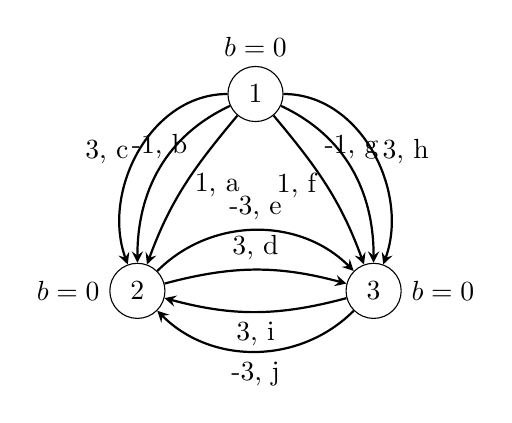
\begin{tikzpicture}[node distance=2.5 cm]
                            \node (1) [circleNode, label=above:{$b = 0$}] {1};
                            \node (2) [circleNode, below of=1, xshift=-1.5 cm, label=left:{$b = 0$}] {2};
                            \node (3) [circleNode, below of=1, xshift=1.5 cm, label=right:{$b = 0$}] {3};
                            \draw [arrow] (1) to [out = 230, in = 70] node [right] {1, a} (2);
                            \draw [arrow] (1) to [out = 205, in = 90] node [above] {-1, b} (2);
                            \draw [arrow] (1) to [out = 180, in = 110] node [left] {3, c} (2);
                            \draw [arrow] (1) to [out = 0, in = 70] node [right] {3, h} (3);
                            \draw [arrow] (1) to [out = -25, in = 90] node [above] {-1, g} (3);
                            \draw [arrow] (1) to [out = -50, in = 110] node [left] {1, f} (3);
                            \draw [arrow] (2) to [out = 15, in = 165] node [above] {3, d} (3);
                            \draw [arrow] (2) to [out = 45, in = 135] node [above] {-3, e} (3);
                            \draw [arrow] (3) to [out = -165, in = -15] node [below] {3, i} (2);
                            \draw [arrow] (3) to [out = -135, in = -45] node [below] {-3, j} (2);
                        \end{tikzpicture}
                    \end{figure}

                    Then for the following steps we can detect cycling:

                    \begin{itemize}
                        \item $w(T, j) = w_j - w_i = -3 -3 = -6$, therefore $j$ in entering basis, $i$ is leaving basis.
                        \item $w(T, h) = w_h + w_j - w_a = 3-3-1=-1$, therefore $h$ is entering basis, $a$ is leaving basis.
                        \item $w(T, b) = w_b - w_j - w_h = -1 + 3 - 3 = -1$, therefore $b$ is entering basis, $j$ is leaving basis.
                        \item $w(T, d) = w_d - w_h + w_b = 3 - 3 - 1 = -1$, therefore $d$ is entering basis, $h$ is leaving basis.
                        \item $w(T, f) = w_f - w_d - w_b = 1 - 3 + 1 = -1$, therefore $f$ is entering basis, $b$ is leaving basis.
                        \item $w(T, e) = w_e - w_d = -3 -3 = -6$, therefore $e$ is entering basis, $d$ is leaving basis.
                        \item $w(T,c) = w_c + w_e - w_f = 3 -3 - 1 = -1$, therefore $c$ is entering basis, $f$ is leaving basis.
                        \item $w(T,g) = w_g - w_e - w_c = -1 + 3 - 3 = -1$, therefore $g$ is entering basis, $e$ is leaving basis.
                        \item $w(T,i) = w_i - w_c + w_g =3 - 3 - 1= -1 $, therefore $i$ is entering basis, $c$ is leaving basis.
                        \item $w(T,a) = w_a - w_i - w_g = 1 - 3 + 1 = -1$, therefore $a$ is entering basis, $g$ is leaving basis.                
                    \end{itemize}

                    \begin{figure}
                        \centering
                        \begin{subfigure}[c]{0.24\textwidth}
                            \centering
                            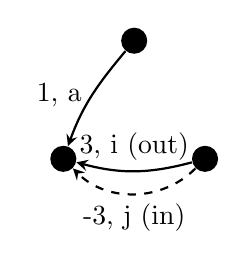
\begin{tikzpicture}[node distance=1.5 cm]
                                \node (1) [solidNode] {};
                                \node (2) [solidNode, below of = 1, xshift=-0.9 cm] {};
                                \node (3) [solidNode, below of = 1, xshift=0.9 cm] {};
                                \draw [arrow] (1) to [out = 230, in = 70] node [left] {1, a} (2);
                                \draw [arrow] (3) to [out = -165, in = -15] node [above] {3, i (out)} (2);
                                \draw [arrow, dashed] (3) to [out = -135, in = -45] node [below] {-3, j (in)} (2);
                            \end{tikzpicture}
                        \end{subfigure}
                        \qquad
                        \begin{subfigure}[c]{0.24\textwidth}
                            \centering
                            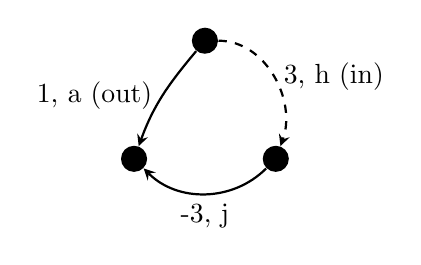
\begin{tikzpicture}[node distance=1.5 cm]
                                \node (1) [solidNode] {};
                                \node (2) [solidNode, below of = 1, xshift=-0.9 cm] {};
                                \node (3) [solidNode, below of = 1, xshift=0.9 cm] {};
                                \draw [arrow] (1) to [out = 230, in = 70] node [left] {1, a (out)} (2);
                                \draw [arrow] (3) to [out = -135, in = -45] node [below] {-3, j} (2);
                                \draw [arrow, dashed] (1) to [out = 0, in = 70] node [right] {3, h (in)} (3);
                            \end{tikzpicture}
                        \end{subfigure}
                        \qquad
                        \begin{subfigure}[c]{0.24\textwidth}
                            \centering
                            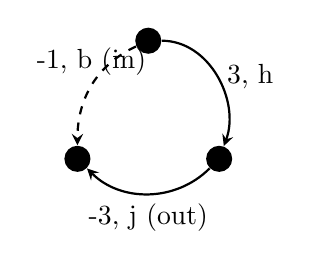
\begin{tikzpicture}[node distance=1.5 cm]
                                \node (1) [solidNode] {};
                                \node (2) [solidNode, below of = 1, xshift=-0.9 cm] {};
                                \node (3) [solidNode, below of = 1, xshift=0.9 cm] {};
                                \draw [arrow, dashed] (1) to [out = 205, in = 90] node [above] {-1, b (in)} (2);
                                \draw [arrow] (1) to [out = 0, in = 70] node [right] {3, h} (3);
                                \draw [arrow] (3) to [out = -135, in = -45] node [below] {-3, j (out)} (2);
                            \end{tikzpicture}
                        \end{subfigure}
                        \qquad
                        \begin{subfigure}[c]{0.24\textwidth}
                            \centering
                            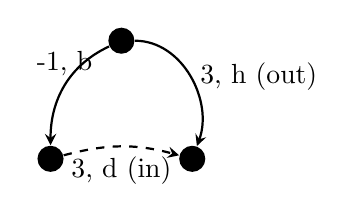
\begin{tikzpicture}[node distance=1.5 cm]
                                \node (1) [solidNode] {};
                                \node (2) [solidNode, below of = 1, xshift=-0.9 cm] {};
                                \node (3) [solidNode, below of = 1, xshift=0.9 cm] {};
                                \draw [arrow] (1) to [out = 205, in = 90] node [above] {-1, b} (2);
                                \draw [arrow] (1) to [out = 0, in = 70] node [right] {3, h (out)} (3);
                                \draw [arrow, dashed] (2) to [out = 15, in = 165] node [below] {3, d (in)} (3);
                            \end{tikzpicture}
                        \end{subfigure}
                        \qquad
                        \begin{subfigure}[c]{0.24\textwidth}
                            \centering
                            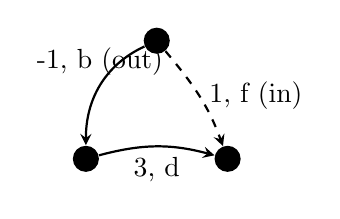
\begin{tikzpicture}[node distance=1.5 cm]
                                \node (1) [solidNode] {};
                                \node (2) [solidNode, below of = 1, xshift=-0.9 cm] {};
                                \node (3) [solidNode, below of = 1, xshift=0.9 cm] {};
                                \draw [arrow] (1) to [out = 205, in = 90] node [above] {-1, b (out)} (2);
                                \draw [arrow, dashed] (1) to [out = -50, in = 110] node [right] {1, f (in)} (3);
                                \draw [arrow] (2) to [out = 15, in = 165] node [below] {3, d} (3);
                            \end{tikzpicture}
                        \end{subfigure}
                        \qquad
                        \begin{subfigure}[c]{0.24\textwidth}
                            \centering
                            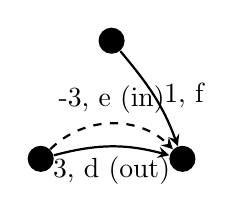
\begin{tikzpicture}[node distance=1.5 cm]
                                \node (1) [solidNode] {};
                                \node (2) [solidNode, below of = 1, xshift=-0.9 cm] {};
                                \node (3) [solidNode, below of = 1, xshift=0.9 cm] {};
                                \draw [arrow] (1) to [out = -50, in = 110] node [right] {1, f} (3);
                                \draw [arrow] (2) to [out = 15, in = 165] node [below] {3, d (out)} (3);
                                \draw [arrow, dashed] (2) to [out = 45, in = 135] node [above] {-3, e (in)} (3);
                            \end{tikzpicture}
                        \end{subfigure}
                        \qquad
                        \begin{subfigure}[c]{0.24\textwidth}
                            \centering
                            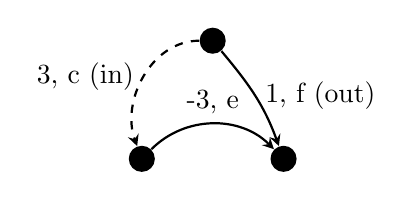
\begin{tikzpicture}[node distance=1.5 cm]
                                \node (1) [solidNode] {};
                                \node (2) [solidNode, below of = 1, xshift=-0.9 cm] {};
                                \node (3) [solidNode, below of = 1, xshift=0.9 cm] {};
                                \draw [arrow, dashed] (1) to [out = 180, in = 110] node [left] {3, c (in)} (2);
                                \draw [arrow] (1) to [out = -50, in = 110] node [right] {1, f (out)} (3);
                                \draw [arrow] (2) to [out = 45, in = 135] node [above] {-3, e} (3);
                            \end{tikzpicture}
                        \end{subfigure}
                        \qquad
                        \begin{subfigure}[c]{0.24\textwidth}
                            \centering
                            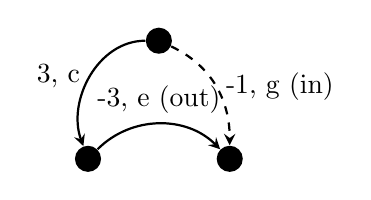
\begin{tikzpicture}[node distance=1.5 cm]
                                \node (1) [solidNode] {};
                                \node (2) [solidNode, below of = 1, xshift=-0.9 cm] {};
                                \node (3) [solidNode, below of = 1, xshift=0.9 cm] {};
                                \draw [arrow, dashed] (1) to [out = -25, in = 90] node [right] {-1, g (in)} (3);
                                \draw [arrow] (1) to [out = 180, in = 110] node [left] {3, c} (2);
                                \draw [arrow] (2) to [out = 45, in = 135] node [above] {-3, e (out)} (3);
                            \end{tikzpicture}
                        \end{subfigure}
                        \qquad
                        \begin{subfigure}[c]{0.24\textwidth}
                            \centering
                            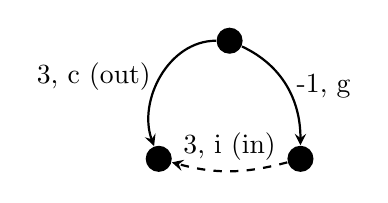
\begin{tikzpicture}[node distance=1.5 cm]
                                \node (1) [solidNode] {};
                                \node (2) [solidNode, below of = 1, xshift=-0.9 cm] {};
                                \node (3) [solidNode, below of = 1, xshift=0.9 cm] {};
                                \draw [arrow] (1) to [out = -25, in = 90] node [right] {-1, g} (3);
                                \draw [arrow] (1) to [out = 180, in = 110] node [left] {3, c (out)} (2);
                                \draw [arrow, dashed] (3) to [out = -165, in = -15] node [above] {3, i (in)} (2);
                            \end{tikzpicture}
                        \end{subfigure}
                        \qquad
                        \begin{subfigure}[c]{0.24\textwidth}
                            \centering
                            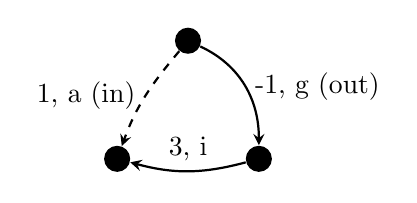
\begin{tikzpicture}[node distance=1.5 cm]
                                \node (1) [solidNode] {};
                                \node (2) [solidNode, below of = 1, xshift=-0.9 cm] {};
                                \node (3) [solidNode, below of = 1, xshift=0.9 cm] {};
                                \draw [arrow, dashed] (1) to [out = 230, in = 70] node [left] {1, a (in)} (2);
                                \draw [arrow] (1) to [out = -25, in = 90] node [right] {-1, g (out)} (3);
                                \draw [arrow] (3) to [out = -165, in = -15] node [above] {3, i} (2);
                            \end{tikzpicture}
                        \end{subfigure}
                        \qquad
                        \begin{subfigure}[c]{0.24\textwidth}
                            \centering
                            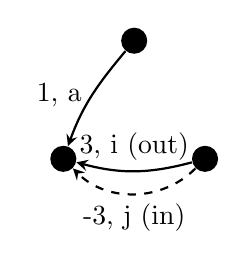
\begin{tikzpicture}[node distance=1.5 cm]
                                \node (1) [solidNode] {};
                                \node (2) [solidNode, below of = 1, xshift=-0.9 cm] {};
                                \node (3) [solidNode, below of = 1, xshift=0.9 cm] {};
                                \draw [arrow] (1) to [out = 230, in = 70] node [left] {1, a} (2);
                                \draw [arrow] (3) to [out = -165, in = -15] node [above] {3, i (out)} (2);
                                \draw [arrow, dashed] (3) to [out = -135, in = -45] node [below] {-3, j (in)} (2);
                            \end{tikzpicture}
                        \end{subfigure}
                    \end{figure}

                    The last graph is the same as the first graph, i.e., cycling detected.

                \paragraph{Cycling prevention}
                    To Avoid cycling we will introduce the Modified Network Simplex Method. Let $T$ be a \textbf{rooted} spanning tree. Let $f$ be an arc in $T$, we say $f$ is \textbf{away} from the root $r$ if $t(f)$ is the component of $T-f$. Otherwise we say $f$ is \textbf{towards} $r$.

                    Let $x$ be a feasible tree solution associated with $T$, then we say $T$ is a \textbf{strong feasible tree} if for every arc $f \in T$ with $x_f = 0$ then $f$ is away from $r\in T$.

                    Modification to NSM:
                    \begin{itemize}
                        \item The algorithm is initialed with a strong feasible tree.
                        \item $f$ in pivot phase is chosen to be the first reverse arc of $C(T, e)$ having $x_f = \theta$. By ``first'', we mean the first arc encountered in traversing $C(T, e)$ in the direction of $e$, starting at the vertex $i$ of $C(T, e)$ that minimizes the number of arcs in the unique $(r, i)$-path in $T$.
                    \end{itemize}

                    In the second rule above, $r$ could also be in the cycle, in that case, $i$ is $r$.

                    Continue the previous example. Now should how we can avoid cycling:

                    The first few (four) steps are the same as previous example, starting from

                    \begin{figure}[H]
                        \centering
                        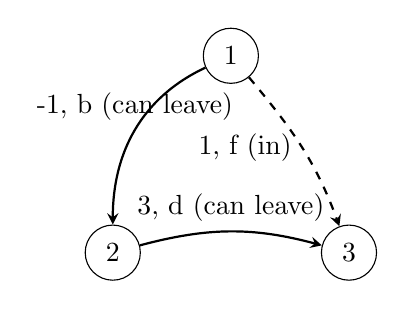
\begin{tikzpicture}[node distance=2.5 cm]
                            \node (1) [circleNode] {1};
                            \node (2) [circleNode, below of = 1, xshift=-1.5 cm] {2};
                            \node (3) [circleNode, below of = 1, xshift=1.5 cm] {3};
                            \draw [arrow] (1) to [out = 205, in = 90] node [above] {-1, b (can leave)} (2);
                            \draw [arrow, dashed] (1) to [out = -50, in = 110] node [left] {1, f (in)} (3);
                            \draw [arrow] (2) to [out = 15, in = 165] node [above] {3, d (can leave)} (3);
                        \end{tikzpicture}
                    \end{figure}

                    $w(T,f) = w_f - w_d - w_b = 1 - 3 + 1 = -1$. $f$ is entering basis, both $b$ and $d$ can leave the basis, according to the modified pivot rule, we choose the ``first'' arc encountered in traversing $C(T, e)$, which is $d$ to leave the basis, instead of $b$.

                    \begin{figure}[H]
                        \centering
                        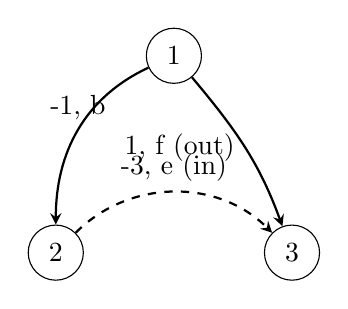
\begin{tikzpicture}[node distance=2.5 cm]
                            \node (1) [circleNode] {1};
                            \node (2) [circleNode, below of = 1, xshift=-1.5 cm] {2};
                            \node (3) [circleNode, below of = 1, xshift=1.5 cm] {3};
                            \draw [arrow] (1) to [out = 205, in = 90] node [above] {-1, b} (2);
                            \draw [arrow] (1) to [out = -50, in = 110] node [left] {1, f (out)} (3);
                            \draw [arrow, dashed] (2) to [out = 45, in = 135] node [above] {-3, e (in)} (3);
                        \end{tikzpicture}
                    \end{figure}

                    $w(T, e) = w_e - w_f + w_b = -5$, $e$ is entering basis, $f$ is leaving basis. Now the only arc to enter basis and maintain negative $w$ is $j$.

                    \begin{figure}[H]
                        \centering
                        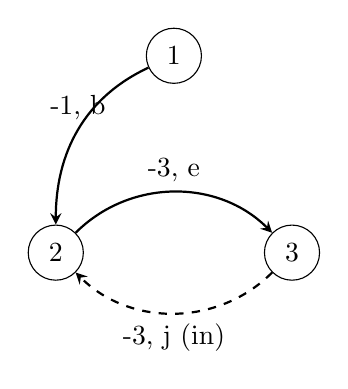
\begin{tikzpicture}[node distance=2.5 cm]
                            \node (1) [circleNode] {1};
                            \node (2) [circleNode, below of = 1, xshift=-1.5 cm] {2};
                            \node (3) [circleNode, below of = 1, xshift=1.5 cm] {3};
                            \draw [arrow] (1) to [out = 205, in = 90] node [above] {-1, b} (2);
                            \draw [arrow] (2) to [out = 45, in = 135] node [above] {-3, e} (3);
                            \draw [arrow, dashed] (3) to [out = -135, in = -45] node [below] {-3, j (in)} (2);
                        \end{tikzpicture}
                    \end{figure}

                    $w(T, j) = w_j + w_e = -6$, but in $C(T, j)$ there is no reversing arc, therefore we detect unboundness.

                \paragraph{Finding Initial Strong Feasible Tree}
                    Pick a vertex in $D$ to be root $r$. The tree $T$ has an arc $e$ with the $t(e) = r$ and $h(e) = v$. For each $v\in V\setminus r$ with $b_v \ge 0$ and has an arc $e$ with $h(e) = r$ and $t(e) = v$ for each $v \in V\setminus r$ for which $b_v < 0$. Wherever possible the arcs of $T$ are chosen from $A$, where an appropriate arc doesn't exist. We create an \textbf{artificial arc} and give its weight $|V|(\max\{w_e: e\in A\}) + 1$. This is similar to Big-M method and if optimal solution contains artificial arcs ongoing arc problem is infeasible.

                    Here is an example after adding artificial arcs:

                    \begin{figure}[H]
                        \centering
                        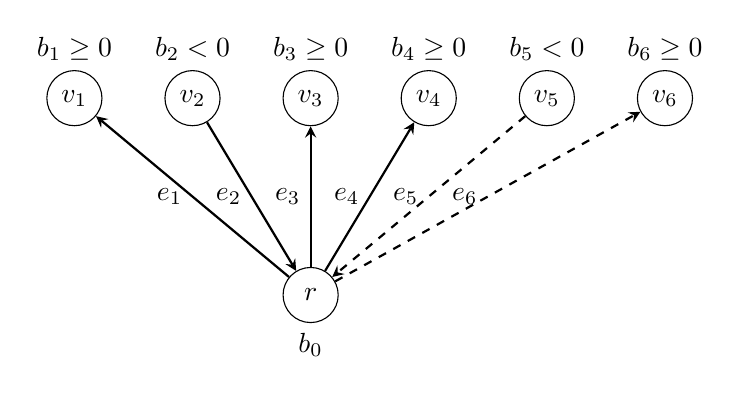
\begin{tikzpicture}[node distance = 1.5 cm]
                            \node (1) [circleNode, label=above:{$b_1 \ge 0$}] {$v_1$};
                            \node (2) [circleNode, label=above:{$b_2 < 0$}, right of = 1] {$v_2$};
                            \node (3) [circleNode, label=above:{$b_3 \ge 0$}, right of = 2] {$v_3$};
                            \node (4) [circleNode, label=above:{$b_4 \ge 0$}, right of = 3] {$v_4$};
                            \node (5) [circleNode, label=above:{$b_5 < 0$}, right of = 4] {$v_5$};
                            \node (6) [circleNode, label=above:{$b_6 \ge 0$}, right of = 5] {$v_6$};
                            \node (0) [circleNode, label=below:{$b_0$}, below of= 3, yshift=-1 cm] {$r$};
                            \draw [arrow] (0) -- node [left] {$e_1$} (1);
                            \draw [arrow] (2) -- node [left] {$e_2$} (0);
                            \draw [arrow] (0) -- node [left] {$e_3$} (3);
                            \draw [arrow] (0) -- node [left] {$e_4$} (4);
                            \draw [arrow, dashed] (5) -- node [left] {$e_5$} (0);
                            \draw [arrow, dashed] (0) -- node [left] {$e_6$} (6);
                        \end{tikzpicture}
                    \end{figure}

                    Where $e_5$ and $e_6$ are artificial arcs, the weight of those arcs are $|V|(\max\{w_e: e\in \mathcal{A}\}) + 1$. And the above tree is a basic feasible solution.

                    We need to prove that such artificial arc has sufficiently large weight to guarantee

                    \begin{itemize}
                        \item It will leave the basis, and
                        \item It will not enter the basis again (for this, just delete the artificial arc after it leaves the basis, then it will never enter the basis again)
                    \end{itemize}

                    \begin{proof}
                        Now prove that such arcs will always leave the basis. Before the prove we give some notation. 
                        \begin{itemize}
                            \item Define set $E$ as the set of arcs which is not artificial arc, in the above example, $E = \{e_1, e_2, e_3, e_4\}$. 
                            \item Define set $A$ as the set of arcs which are artificial arcs, in the above example, $A = \{e_5, e_6\}$. Noticed that $E \cap A = \emptyset$.
                            \item Define set $M$ as the vertices in the spanning tree that is reachable from $r$ by $E$, in the above example, $M = \{v_1, v_2, v_3, v_4\}$.
                            \item Define $M^\prime = (V\setminus r) \setminus M$ in the tree that can only be reached from $r$ by $A$, i.e., artificial arcs, in the above example, $M^\prime = \{v_5, v_6\}$. 
                        \end{itemize}

                        Then the initial basic feasible solution is a graph 
                        \begin{equation*}
                            G_0 = <M\cup M^\prime \cup \{r\}, E\cup A>
                        \end{equation*}
                        Denote the origin graph 
                        \begin{equation*}
                            G = <V, \mathcal{A}>
                        \end{equation*}
                        Notice that with the artificial arcs, $G_0$ is not a subgraph of $G$.

                        Let $(M\cup\{r\}, M^\prime)$ be a cut in the origin graph $G$. For the vertices in $M^\prime$, one of the following cases will happen:
                        \begin{itemize}
                            \item case 1: $\sum_{v \in M^\prime} b_v \ge 0$
                            \item case 2: $\sum_{v \in M^\prime} b_v < 0$
                        \end{itemize}

                        For case 1, we claim that at least one of the vertices $v_{M^\prime} \in M^\prime$ with $b_{v_{M^\prime}} \ge 0$ linked by an arc, say $f$, such that $h(f) = v_{M^\prime}$ and $t(f) = v_M \in M$. Otherwise the balance of flow cannot hold in the origin graph $G$. Furthermore, denote the artificial arc from $r$ to $v_{M^\prime}$ by $e_{rv_{M^\prime}}$.

                        Notice that for $v_M$ there is not necessarily be an arc between $r$ and $v_M$, but there must exists an $(r, v_M)$-path denoted by $P$, for $M$ is the set of vertices that reachable from $r$ by arcs in $E$.

                        Take that arc $f$ as entering arc to the basis. Then 
                        \begin{equation*}
                            C(T, f) = re_{rv_{M^\prime}}v_{M^\prime}fv_MPr
                        \end{equation*}
                        For
                        \begin{equation*}
                            w(T, f) = w_f - w_{e_{rv_{M^\prime}}} + \sum_{e \in P} d_e w_e
                        \end{equation*}
                        where $d_e = 1$ if $w_e$ is forward in $P$ and $d_e = -1$ otherwise.

                        Now that $w_{e_{rv_{M^\prime}}} = |V|(\max\{w_e: e\in \mathcal{A}\}) + 1$, it guarantees that
                        \begin{align*}
                            w(T, f) &= w_f + \sum_{e \in P} d_e w_e - w_{e_{rv_{M^\prime}}}\\
                                    &\le w_f + \sum_{e \in P}w_e - w_{e_{rv_{M^\prime}}}\\
                                    &\le \sum_{e \in \mathcal{A}}w_e - w_{e_{rv_{M^\prime}}}\\
                                    &\le |V|(\max\{w_e: e\in \mathcal{A}\}) - w_{e_{rv_{M^\prime}}}\\
                                    &\le -1 < 0 
                        \end{align*}
                        So $f$ can enter the basis, and the artificial variable $e_{rv_{M^\prime}}$ will leave the basis, for it is the most violated reverse arc in the $C(T, f)$. When we put $f$ into the basis, update $G_0$, such that $M \leftarrow M \cup \{v_{M^\prime}\}$ and $M^\prime \leftarrow M^\prime \setminus \{v_{M^\prime}\}$.

                        For case 2, it is similar. At least one of the vertices $v_{M^\prime} \in M^\prime$ with $b_{v_{M^\prime}} < 0$ linked by an arc, say $f\prime$, such that $t(f^\prime) = v_{M^\prime}$ and $h(f^\prime) = v_M \in M$. Otherwise the balance of flow cannot hold in the origin graph $G$. Furthermore, denote the artificial arc from $v_{M^\prime}$ to $r$ by $e_{v_{M^\prime}r}$.

                        Similarly we can find a cycle $C(T, f^\prime) = rP^\prime v_M f^\prime v_{M^\prime}e_{v_{M^\prime}r}r$. $w(T, f^\prime) = w_{f^\prime} - w_{e_{rv_{M^\prime}}} + \sum_{e \in P^\prime} d_e w_e$, where $d_e = 1$ if $w_e$ is forward in $P\prime$ and $d_e = -1$. We can prove $w(T, f^\prime) \le -1 < 0$. That that $f^\prime$ as entering arc to the basis, similarly move $v_{M^\prime}$ form set $M^\prime$ to $M$.

                        The above case can be dealt with iteratively until set $M^\prime$ become $\emptyset$, at which stage there is no artificial arc in the basic feasible solution. Which means all the artificial variable can leave the basis.
                    \end{proof}

    \chapter{Traveling Salesman Problem}
        \begin{center}
            \textit{``O never go back.''}
        \end{center}

        \section{The Traveling Salesman Problem}
            In this section, we are going to compare between different formulations of the Traveling Salesman Problem (TSP). Generally speaking, let $G = (V, A)$ be a graph where $V$ is a set of $n$ vertices, and $A$ is a set of arcs (or edges). Let $C = c_{ij}$ be a cost (distance) matrix associated with $A$. The TSP consists of determining a minimum cost (distance) Hamiltonian circle (or cycle) that visits each vertex once and only once. If for all $i, j \in V, c_{ij} = c_{ji}$, then the TSP is symmetrical, otherwise is asymmetrical.

            Define the decision variable $x_{ij}$ as the following
            \begin{equation}
                x_{ij} = \begin{cases}
                    1, &\text{if goes from } i \text{ to } j\\ 
                    0, & \text{otherwise}
                \end{cases}, \quad (i, j) \in A
            \end{equation}

            The objective function is
            \begin{equation}
                \min \quad \sum_{(i, j)\in A} c_{ij}x_{ij}
            \end{equation}

            \subsection{Dantzig-Fulkerson-Johnson (DFJ) Formulation}
                The first famous formulations for TSP is the \textbf{Dantzig-Fulkerson-Johnson (DFJ) formulation}:
                \begin{align}
                    \sum_{j \in V, (i,j)\in A} x_{ij} & = 1, \quad \forall i \in V \label{TSP:con:degree1}\\
                    \sum_{i \in V, (i,j)\in A} x_{ij} & = 1, \quad \forall j \in V \label{TSP:con:degree2}\\
                    \sum_{j\notin S, i\in S, (i,j)\in A} x_{ij} & \ge 1, \quad \forall S \subset V, 2\le |S| \le n-1 \label{TSP:con:DFJSubtour1}
                \end{align}

                In the formulation, constraints (\ref{TSP:con:degree1}) and constraints (\ref{TSP:con:degree2}) are degree constraints, which specify that every vertex is entered exactly once. Constraints (\ref{TSP:con:DFJSubtour1}) is the sub-tour constraints, they prohibit the formation of sub-tours. $S$ is a non-empty subset of $V$, and has at least 2 vertices. (\ref{TSP:con:DFJSubtour1}) can be replaced by
                \begin{equation}
                    \sum_{i, j \in S, (i, j) \in A} x_{ij} \le |S| - 1, \quad \forall S \subset V, 2\le |S| \le n-1\label{TSP:con:DFJSubtour2}
                \end{equation}

                If we list all sub-tour constraints in DFJ, there will be $O(2^n)$ constraints and $O(n^2)$ binary variables. The exponential number of constraints makes it impractical to solve directly. Instead, lazy constraints are usually implemented for the sub-tour elimination constraints (\ref{TSP:con:DFJSubtour1}) or (\ref{TSP:con:DFJSubtour2}).

            \subsection{Miller-Tucker-Zemlin (MTZ) Formulation}
                We can also formulate TSP using sequential formulations, namely, \textbf{Miller-Tucker-Zemlin (MTZ) formulation}. In the MTZ formulation, the degree constraints (\ref{TSP:con:degree1}) and (\ref{TSP:con:degree2}) are the same as in DFJ formulation.

                Define a new set of integer decision variables $u_i$, $u_i$ defined as the sequence in which node $i$ is visited, $u_1 = 1$.

                The sub-tour constraints (\ref{TSP:con:DFJSubtour1}) or (\ref{TSP:con:DFJSubtour2}) are replaced by the following:
                \begin{align}
                    u_i - u_j + (n - 1) x_{ij} &\le n - 2, \quad i, j = 2, \cdots, n \in V, (i, j) \in A \label{TSP:con:MTZ1}\\
                    1 & \le u_i \le n - 1, \quad i \in 2, \cdots, n \in V \label{TSP:con:MTZ2}
                \end{align}

                In MTZ formulation, there are $O(n^2)$ constraints, $O(n^2)$ binary variables, and $O(n)$ continuous variables.

            \subsection{Flow Based Formulations}
                In this section, flow based formulations are discussed, which includes \textbf{Single Commodity Flow}, \textbf{Two Commodity Flow} and \textbf{Multi-Commodity Flow}. In these formulations, continuous variables are introduced to represent the flow on the arcs.

                In Single Commodity Flow formulation, define $y_{ij}$ as the flow in an arc $(i, j) \in A$. Degree constraints (\ref{TSP:con:degree1}) and (\ref{TSP:con:degree2}) are retained. The following constraints are introduced:
                \begin{align}
                    y_{ij} & \le (n - 1) x_{ij}, \quad \forall i, j \in V, (i, j) \in A \label{TSP:con:SCFMaxFlow}\\
                    \sum_{j \in V, (1, j) \in A} y_{1j} & = n - 1 \label{TSP:con:SCFInitFlow} \\
                    \sum_{i \in V, (i, j) \in A} y_{ij} - \sum_{k \in V, (j, k) \in A} y_{jk} &= 1, \quad \forall j \in V \setminus \{1\} \label{TSP:con:SCFFlowBalance}
                \end{align}

                Constraints (\ref{TSP:con:SCFMaxFlow}) can be tighten by the following:
                \begin{align}
                    y_{ij} &\le (n - 1) x_{ij}, \quad i = 1, j \in V \setminus \{1\}, (i, j) \in A \label{TSP:con:SCMMaxFlow1} \\
                    y_{ij} &\le (n - 2) x_{ij}, \quad i, j \in V \setminus \{1\}, (i, j) \in A \label{TSP:con:SCMMaxFlow2}
                \end{align}

                In SCM formulation, there are $O(n^2)$ constraints, $O(n^2)$ binary variables and $O(n^2)$ continuous variables.

                In Two Commodity Flow formulation, define $y_{ij}$ as the flow in an arc $(i, j) \in A$, for commodity type 1, and define $z_{ij}$ as the flow in an arc $(i, j) \in A$, for commodity type 2.

                Besides degree constraints, the other constraints are as following
                \begin{align}
                    y_{ij} + z_{ij} &= (n - 1) x_{ij}, \quad \forall i, j \in V, (i, j) \in A \label{TSP:con:TCMFlowExist} \\
                    \sum_{j \in V \setminus \{1\}} (y_{1j} - y_{j1}) &= n - 1, \quad (1, j) \in A \label{TSP:con:TCMInitFlowY}\\
                    \sum_{j \in V} (y_{ij} - y_{ji}) & = 1, \quad  \forall i \in V \setminus \{1\}, (i, j) \in A \label{TSP:con:TCMFlowBalanceY}\\
                    \sum_{j \in V \setminus \{1\}} (z_{1j} - z_{j1}) &= 1 - n, \quad (1, j) \in A \label{TSP:con:TCMInitFlowZ}\\
                    \sum_{j \in V} (z_{ij} - z_{ji}) & = -1, \quad  \forall i \in V \setminus \{1\}, (i, j) \in A \label{TSP:con:TCMFlowBalanceZ}\\
                    \sum_{j \in V} (y_{ij} + z_{ij}) &= n - 1, \quad \forall i \in V \label{TSP:con:TCMFlowOnArc}
                \end{align}

                In TCM formulation, constraints (\ref{TSP:con:TCMFlowExist}) only allow flow in an arc if present. Constraints (\ref{TSP:con:TCMInitFlowY}) and (\ref{TSP:con:TCMFlowBalanceY}) forces $(n - 1)$ units of commodity type 1 to flow in at node 1 and 1 unit to flow out at every other nodes. Constraints (\ref{TSP:con:TCMInitFlowZ}) and (\ref{TSP:con:TCMFlowBalanceZ}) are similar, those forces $(n - 1)$ units of commodity type 2 to flow out at node 1 and 1 unit to flow in at every other nodes. Constraints (\ref{TSP:con:TCMFlowOnArc}) forces exactly $(n - 1)$ units of combined commodity in each arc.

                In TCM formulation, there are $O(n^2)$ constraints, $O(n^2)$ binary variables and $O(n^2)$ continuous variables.

                The SCM and the TCM can be generalized into \textbf{Multi-Commodity Flow formulation}. As usual, degree constraints are retained. The following continuous variables are introduced. Define $y_{ij}^k$ as the flow of commodity type $k$ in arc $(i, j) \in A$.

                The other constraints are
                \begin{align}
                    y_{ij}^k &\le x_{ij}, \quad \forall i, j, k \in N, k \neq 1 \label{TSP:con:MCMFlowExist}\\
                    \sum_{i \in V} y_{1i}^k &= 1, \quad \forall k \in V \setminus \{1\} \label{TSP:con:MCMInitIn}\\
                    \sum_{i \in V} y_{i1}^k &= 0, \quad \forall k \in V \setminus \{1\} \label{TSP:con:MCMInitOut}\\
                    \sum_{i \in V} y_{ik}^k &= 1, \quad \forall k \in V \setminus \{1\} \label{TSP:con:MCMElseOut}\\
                    \sum_{j \in V} y_{kj}^k &= 0, \quad \forall k \in V \setminus \{1\} \label{TSP:con:MCMElseIn}\\
                    \sum_{i \in V} y_{ij}^k - \sum_{i \in V} y_{ji}^k &= 0, \quad \forall j, k \in V \setminus \{1\}, j \neq k \label{TSP:con:MCMBalance}
                \end{align}
                Constraints (\ref{TSP:con:MCMFlowExist}) only allow flow in an arc which is present. Constraints (\ref{TSP:con:MCMInitIn}) forces exactly one unit of each type of commodity to flow in at node 1. Constraints (\ref{TSP:con:MCMInitOut}) prevent any commodity flow out at node 1.Constraints (\ref{TSP:con:MCMElseOut}), and Constraints (\ref{TSP:con:MCMElseIn}), forces exactly one unit of type $k$ commodity to flow out, and in, at every node except node 1. Constraints (\ref{TSP:con:MCMBalance}) forces balance of all types of commodities at every node except node 1.

                This formulation has $O(n^3)$ constraints, $O(n^2)$ binary variables, and $O(n^3)$ continuous variables.

            \subsection{Shortest Path Formulation}
                In this section, we are going to introduce another form of formulation with different definition of decision variable and objective function.

                Assuming for a completed graph $G = (V, A)$. Define $x_{ij}^t$ as the following
                \begin{equation}
                    x_{ij}^t = \begin{cases}
                                    1, \quad \text{If path crosses arc } (i, t) \text{ and } (j, t + 1) \\
                                    0, \quad \text{Otherwise}
                                \end{cases}, \quad i \in V, j \in V \setminus \{i\}, t = 1, \cdots, n
                \end{equation}

                \begin{figure}[!h]
                    \centering
                    \includegraphics[width=0.6\textwidth]{../../image/timeStaged.png}
                    \caption{Time-staged graph}
                    \label{fig:timeStaged}
                \end{figure}

                The objective function will be
                \begin{equation}
                    \min \quad \sum_{i \in V}\sum_{j \in V\setminus \{i\}} c_{ij} \sum_{t = 1}^n x_{ij}^t
                \end{equation}

                The constraints are as following
                \begin{align}
                    \sum_{j \in V \setminus \{1\}} x_{1j}^1 &= 1 \label{TSP:con:SPFStart}\\
                    \sum_{j \in V \setminus \{1, i\}} x_{ij}^2 - x_{1i}^1 &= 0, \quad \forall i \in V \setminus \{1\} \label{TSP:con:SPFFirstLayer}\\
                    \sum_{j \in V \setminus \{1, i\}} x_{ij}^t - \sum_{j \in V \setminus \{1, i\}} x_{ji}^{t - 1} &= 0, \quad \forall i \in V \setminus \{1\}, t \in \{2, \dots, n - 1\} \label{TSP:con:SPFTthLayer}\\
                    x_{i1}^n - \sum_{j \in V \setminus \{1, i\}} x_{ji}^{n - 1} &= 0, \quad \forall i \in V \setminus \{1\} \label{TSP:con:SPFLastLayer}\\
                    \sum_{i \in V \setminus \{1\}} x_{i1}^n &= 1 \label{TSP:con:SPFEnd}\\
                    \sum_{t = 2}^{n - 1}\sum_{j \in V \setminus \{1, i\}} x_{ij}^t + x_{i1}^n & \le 1, \quad \forall i \in V \setminus \{1\} \label{TSP:con:SPFSameType1}
                \end{align}

                Notice that constraint (\ref{TSP:con:SPFSameType1}) can be replaced by
                \begin{equation}
                    x_{1i}^1 + \sum_{t = 2}^{n - 1}\sum_{j \in V \setminus \{1, i\}} x_{ji}^t \le 1, \quad \forall i \in V \setminus \{1\} \label{TSP:con:SPFSameType2}
                \end{equation}

            \subsection{Quadratic Formulation (QAP)}
                In this section, we are going to go over a TSP formulation are super bad. However, it still has some value for further study.

                The idea is to transform TSP into an assignment problem. Assuming we have $n$ boxes, which represents $n$ steps in the path. Define $x_{ij}$ as 
                \begin{equation}
                    x_{ij} = \begin{cases}
                                1, \quad \text{Vertex $i$ is assigned to box $j$}\\
                                0, \quad \text{Otherwise}
                            \end{cases}
                \end{equation}

                The constraints are simple as an assignment problem as following
                \begin{align}
                    \sum_{j = 1}^n x_{ij} &= 1, \quad \forall i \in V\\
                    \sum_{i \in V}^n x_{ij} &= 1, \quad j = 1, \dots, n
                \end{align}

                However, the tricky part is in the objective function
                \begin{equation}
                    \min \quad \sum_{i \in V} \sum_{j \in V \setminus \{i\}} \sum_{k = 1}^{n - 1} c_{ij} x_{ik} x_{j, k + 1} + \sum_{i \in V} \sum_{j \in V \setminus \{i\}} c_{ij}x_{in}x_{j1}
                \end{equation}

                Notice that the objective function is not linear function, with the multiplications of decision variables. Now we are going to linearize them. The linearized version is as following

                \begin{align}
                    \min \quad & \sum_{i \in V} \sum_{j \in V \setminus \{i\}} \sum_{k = 1}^{n - 1} c_{ij} w_{ij}^k + \sum_{i \in V} \sum_{j \in V \setminus \{i\}} c_{ij}w_{ij}^n\\
                    \text{s.t.} \quad & \sum_{j = 1}^n x_{ij} = 1, \quad \forall i \in V\\
                                      & \sum_{i \in V}^n x_{ij} = 1, \quad j = 1, \dots, n\\
                                      & w_{ij}^k \ge x_{ik} + x_{j, k + 1} - 1, \quad i \in V,  j \in V \setminus \{i\}, k = 1, \cdots, n - 1\\
                                      & w_{ij}^k \ge x_{ik} + x_{j1} - 1, \quad i \in V, j \in V \setminus \{i\}, k = n \\
                                      & w_{ij}^k \in \{0, 1\}, \quad i \in V, j \in V \setminus \{i\}, k = 1, \dots, n\\
                                      & x_{ij} \in \{0, 1\}, \quad i \in V, j \in V \setminus \{i\}
                \end{align}

                We can prove that this is very very bad. The optimal solution of the LP Relaxation for the QAP formulation is as follows

                \begin{align}
                    x_{ij} &= \frac{1}{n}, \quad \forall i, j \in V\\
                    w_{ij}^k &= \frac{2}{n} - 1, \quad \forall i \in V, j \in V \setminus \{i\}, k = 1, 2, \ldots, n
                \end{align}

                The solution indicates that all decision variables are symmetric in the LP Relaxation, thus, it did not provide any information for branching. In fact, such formulation will search all $O(2^n)$ branches and the lower bound will be difficult to converge.

            \subsection{Numerical Comparisons}
            
                The following results are on Intel(R) Core(TM) i7-8750H CPU @ 2.20GHz, 2208 Mhz. with Gurobi version 9.3.0. Using this processor, DFJ, MTZ, multi-commodity flow methods can solve instances up to 70 nodes within 10 minutes. Shortest path formulation can solve to optimality for less than 50 nodes within 10 minutes. QAP has the worse performances, which cannot even solve TSP with 15 nodes to optimality within 10 minutes. Here are several observations
                \begin{itemize}
                    \item In general DFJ formulation is the best formulation between DFJ, MTZ, multi-commodity flow, shortest path, and QAP formulations. Both plain loop and lazy cut methods can solve instances that we are studying within 1 second. Which is significantly better than others.
                    \item As per run time, we can sort the performance of formulations as following: DFJ (Lazy cut) $<$ DFJ (Plain Loop) $<$ MTZ $<$ multi-commodity flow $<$ shortest path $<$ QAP.
                \end{itemize}
        
        \section{The Held and Karp Lower Bound}
            In this section, we will solve the Dantzig-Fulkerson-Johnson formulation using Lagrangian Relaxation. Before finally converge, the LR finds an infeasible solution as lower bound. The bound found by this method is also known as Held \& Karp Bound.
            
            \subsection{1-Tree}
                We first introduce an intuitive lower bound for TSP, which is the Minimum Spanning Tree Lower Bound. As we known, an optimal solution for the TSP is a Hamilton Cycle which enumerated all vertices on the graph. The length of such Hamilton cycle is denoted as $TSP^*$. If we randomly remove one of the edges, e.g., $\{vw\}$, then, the cycle becomes a path, denoted by $TSP - \{vw\}$. In this case, the degree of vertices $v$ and $w$ reduce to 1 while all the other vertices remains the same as 2. By definition, such path $TSP - \{vw\}$ is a spanning tree on graph $G$. Therefore, the minimum spanning tree of graph $G$ defines a lower bound.

                \begin{equation*}
                    MST \le \text{spanning tree} = TSP - \{vw\} < TSP^*
                \end{equation*}

                We can further improve the lower bound by introducing 1-tree. A spanning tree is a tree with no cycle, if the graph has 1 cycle, it is called 1-tree. Notice that a Hamilton Cycle has only 1 cycle, thus, the Hamilton Cycle is an 1-tree as well. Naturally, the length of all edges of any 1-tree is larger than the length of all edges of the minimum spanning tree. The lower bound of TSP is further improved as follows

                \begin{equation*}
                    MST < M1T \le 1-tree \le TSP^*
                \end{equation*}

                The following algorithm defines an 1-Tree on graph $G$ corresponding to vertex $v$.

                \begin{algorithm}
                    \caption{1-Tree}
                    \begin{algorithmic}
                        \Require A connected graph
                        \Ensure A minimum 1-Tree
                        \State Remove $v$ from the graph
                        \State Use Kroskal's algorithm or Prim's Algorithm to find the minimum spanning tree of $G \setminus \{v\}$
                        \State Find the shortest edge induced by $v$ to the rest of graph $G \setminus \{v\}$, denoted by $vu$ and $vw$, add them to the MST
                        \State \Return 1-Tree
                    \end{algorithmic}
                \end{algorithm}

                \begin{figure}[!htp]
                    \centering                
                    \subfloat[Remove $v$]{\includegraphics[width=0.27\textwidth]{../../image/1Tree1.png}}\quad
                    \subfloat[Find MST]{\includegraphics[width=0.27\textwidth]{../../image/1Tree2.png}}\quad
                    \subfloat[Add back $v$]{\includegraphics[width=0.27\textwidth]{../../image/1Tree3.png}}
                    \caption{Steps in finding minimum 1-Tree}
                    \label{fig:1tree}
                \end{figure}

                A M1T is a good lower bound, however, we can still further improve the lower bound by finding 1-trees.

            \subsection{Held and Karp Lower Bound and Lagrangian Relaxation}
                Notice that in the minimum 1-tree example, vertices have different degrees, some are of degree 1, 2, 3, or more. However, the ``optimal'' 1-tree that we look for, is an 1-tree such that all the vertices are of degree 2. By intuition, if an 1-tree has fewer ``branches'', it's closer to be ``optimal''. That is actually the principle of the Held and Karp Lower Bound.

                We first look at the DFJ formulation for the TSP.

                \begin{align}
                    \min \quad &\sum_{e \in E} \tau_e x_e \label{lr:obj}\\
                    \text{s.t.} \quad & \sum_{e \in \delta(i)} x_e = 2, \quad \forall i \in 1, 2, \ldots, n\label{lr:deg}\\
                    & \sum_{e \in E(S)} x_e \le |S| - 1, \quad \forall S \subset V, 2 \le |S| \le n - 1 \label{lr:subtour}\\
                    & x_e \in \{0, 1\}, \quad \forall e \in E
                \end{align}

                In the DFJ model, the objective is to sum up all the cost of the edges that are chosen on the TSP path. Constraints (\ref{lr:deg}) is a flow balancing constraint, the index $e\in \delta(i)$ represents all the edges that are induced by vertex $i$. Constraints (\ref{lr:subtour}) is the sub-tour constraint.

                Replace the Constraints (\ref{lr:deg}) by the following
                \begin{align}
                    \sum_{e \in \delta(i)} x_e &= 2, \quad \forall i \in 1, 2, \ldots, n - 1\\
                    \sum_{e \in E} x_e &= n
                \end{align}

                We can reformulate the DFJ formulation as follows:

                \begin{align}
                    \min \quad &\sum_{e \in E} \tau_e x_e\\
                    \text{s.t.} \quad & \sum_{e \in \delta(i)} x_e = 2, \quad \forall i \in 1, 2, \ldots, n - 1\label{lr:ndeg}\\
                    &\sum_{e \in E} x_e = n \label{lr:cycle}\\
                    & \sum_{e \in E(S)} x_e \le |S| - 1, \quad \forall S \subset V, 2 \le |S| \le n - 1 \label{lr:nsubtour}\\
                    & x_e \in \{0, 1\}, \quad \forall e \in E
                \end{align}

                Look closely, Constraints (\ref{lr:cycle}) means, the number of edges in the subgraph should be the same as the number of vertices, so the subgraph has 1 cycle. The Constraints (\ref{lr:nsubtour}) guarantee that the graph is connected. Which means, Constraints (\ref{lr:cycle}) and (\ref{lr:nsubtour}) finds an 1-tree.

                Until now, we can move the Constraints (\ref{lr:ndeg}) to the objective function, and use the Lagrangian Relaxation to solve the problem

                \begin{align}
                    z(\mathbf{u}) = \min \quad & \sum_{e \in E} \tau_e x_e + \sum_{i = 1}^{n - 1}u_i(2 - \sum_{e \in \delta(i)} x_e)\\
                    \text{s.t.} \quad & \mathbf{x} \text{ defines an 1-tree with vertice } n
                \end{align}

                For the vertex $i$, define $u_i$, the formulation can be further rewritten as

                \begin{align}
                    z(\mathbf{u}) = \min \quad & 2\sum_{i = 1}^{n - 1} u_i + \sum_{e \in \delta(i)} (\tau_e - u_{e^+} - u_{e^-})x_e\\
                    \text{s.t.} \quad & \mathbf{x} \text{ defines an 1-tree with vertice } n
                \end{align}

            \subsection{Subgradient Descendant Method}
                Notice that in the previous section, we derived a function $z(\mathbf{u})$ of Lagrangian scalar $u_i$ as the lower bound of the TSP. The solution space of $\mathbf{u}$ is a convex space, in this section, we will search the $\max_{\mathbf{u}} z(\mathbf{u})$ by subgradient descendant method.

                \begin{algorithm}
                    \caption{Subgradient descendant method for Held-Karp Lower Bound}
                    \begin{algorithmic}
                        \Require A connected graph
                        \Ensure A lower bound of TSP
                        \State Initialize, for each vertex $i$, let $u_i = 0$, $d_i = \emptyset$. Define lower bound $L \gets 0$, $L^\prime \gets 0$
                        \While $|L - L^\prime| \ge \epsilon$
                            \State Update weights of edges $\tau_{ij} = \tau_{ij} - u_i - u_j$
                            \State Find the M1T on the graph $G$ with edges updated. Let $D$ be the summation of the length of all edges, let $d_i$ be the degree of vertex $i$ on the M1T.
                            \State Update $u_i \gets u_i + \lambda_i \frac{UB - D}{\sum_i (d_i - 2)^2}$
                            \State Update $L^\prime \gets L$
                            \State Update $L \gets D + 2 \sum_i u_i$
                        \EndWhile
                        \State \Return L
                    \end{algorithmic}
                \end{algorithm}

                In the algorithm, different descendant function may be applied, for example, an easier way for implementation is to update
                \begin{equation*}
                    u_i \gets u_i + (d_i - 2) \rho^k
                \end{equation*}

        % \section{Classic Heuristics and Metaheuristics for TSP and VRP}
        %     \subsection{Constructive heuristics}
        %         \paragraph{Nearest neighborhood method}

        %         \paragraph{Insertion method}

        %         \paragraph{Saving method}

        %         \paragraph{Sweep method}

        %         \paragraph{Christofides algorithm}

        %     \subsection{Improvement heuristics}
        %         \paragraph{Relocate}

        %         \paragraph{Or-exchange}

        %         \paragraph{Exchange}

        %         \paragraph{$\lambda$-opt (2-opt, 3-opt)}

        %         \paragraph{Insert}

        %         \paragraph{CROSS}

        %         \paragraph{Swap}

        %         \paragraph{$\lambda$-interchange}

        %         \paragraph{2-opt*}

        %     \subsection{Metaheuristics}
        %         \paragraph{Iterated Local Search}

        %         \paragraph{Large Neighborhood Search}

        %         \paragraph{Simulated Annealing}

        %         \paragraph{Genetic Algorithm}

        %         \paragraph{Ant Colony Algorithm}

        %         \paragraph{Memetic Algorithm}

    \chapter{Column Generation}
        \begin{center}
            \textit{``Stepping bravely into the unknown.''}
        \end{center}

        \section{Fundamental Idea of the Column Generation}
            We first introduce an intuitive approach based on the Revised Simplex Method. Recall the Minkowski-Weyl Theorem

            \begin{theorem}[Minkowski-Weyl Theorem]
                Let $P = \{x \in \mathbb{R}^n | Ax \le b\}$ be a polyhedron with extreme points $V(P) = \{\mathbf{v}_1, \mathbf{v}_2, \cdots, \mathbf{v}_{|V|}\}$ and extreme directions $R(P) = \{\mathbf{r}_1, \mathbf{r}_2, \cdots, \mathbf{r}_{|R|}\}$, then
                \begin{align*}
                    P = \{x \in \mathbb{R}^n |& x = \sum_{j = 1}^{|V|} \lambda_j \mathbf{v}_j + \sum_{j = 1}^{|R|} \mu_j \mathbf{r}_j \\
                    & \sum_{j = 1}^{|V|} \lambda_j = 1, \lambda_j \ge 0, \quad \forall j = 1, 2, \cdots, |V| \\
                    & \mu_j \ge 0, \quad \forall j = 1, 2, \cdots, |R|\}
                \end{align*}
            \end{theorem}

            With out lost of generality, a (bounded) linear problem model can be formulated as follows

            \begin{align*}
                \text{(MP)} \quad  z_{MP}^* = \min \quad & \sum_{j \in J} c_j \lambda_j\\
                \text{s.t.} \quad & \sum_{j \in J} \mathbf{a}_j \lambda_j \ge \mathbf{b} \quad [\mathbf{\pi}]\\
                &\lambda_j \ge 0, \quad \forall j \in J
            \end{align*}

            Where each $\lambda_j$ represents an extreme point of the polyhedron. We call this formulation the master problem (MP). The Revise Simplex Method allows us to solve the LP with a \textbf{large} $|J|$, which is, in each iteration add one more nonbasic variable with negative reduce cost into the formulation. Since we do not need to consider all variables in the beginning, we can start with solving a restricted version of the master problem with only a subset of $J$ (in fact, we can start the iteration with a $B^{-1}$, which is any basic feasible solution). That is

            \begin{align*}
                \text{(RMP)} \quad  z_{RMP}^* = \min \quad & \sum_{j \in J^\prime} c_j \lambda_j\\
                \text{s.t.} \quad & \sum_{j \in J^\prime} \mathbf{a}_j \lambda_j \ge \mathbf{b} \quad [\mathbf{\pi}]\\
                &\lambda_j \ge 0, \quad \forall j \in J^\prime \subset J
            \end{align*}

            We call this formulation the restricted master problem (RMP). In the RMP, we have less choices than the MP, therefore, as a minimization problem, 

            \begin{equation*}
                z_{RMP}^* \ge z_{MP}^*
            \end{equation*}

            provides an upper bound for MP. In each iteration, a new variable - column - is introduced into the formulation, thus, this approach is called the Column Generation.

            \begin{algorithm}[!htp]
                \centering
                \caption{Column generation with explicit pricing}
                \begin{algorithmic}
                    \State Initialize with a set $J^\prime \subseteq J$ of variables
                    \Repeat
                        \State Solve RMP to optimality, obtain $\lambda$ and $\pi$
                        \State Calculate $\bar{c}_j = z_j - c_j = \mathbf{\pi^\top a_j} - c_j, \forall j \in J$
                        \If {$\exists \lambda_{j^*}$ with $z_{j^*} - c_{j^*} < 0$}
                            \State $J^\prime \gets J^\prime \cup \{j^*\}$
                        \EndIf
                    \Until {$\forall \lambda_j, j \in J, z_j - c_j \ge 0$}
                \end{algorithmic}
            \end{algorithm}
            
            Notice that if $|J|$ is \textbf{huge}, it will be just too costly to calculate the reduce cost for \textit{every} nonbasic variable, sometimes (in fact, most of the times) we are not even able to enumerate all nonbasic variables, as the size of $J$ is usually exponentially large. Thus, an optimization problem is introduced to find the least-reduce-cost nonbasic variable, to replace the explicit pricing of all nonbasic variables, we call it the \textit{pricing subproblem}. The updated Column Generation algorithm is as follows

            \begin{algorithm}[!htp]
                \centering
                \caption{Column generation with pricing subproblem}
                \begin{algorithmic}
                    \State Initialize with a set $J^\prime \subseteq J$ of variables
                    \Repeat
                        \State Solve RMP to optimality, obtain $\lambda$ and $\pi$
                        \State Solve $\bar{c}_{j^*} = \min \{z_j - c_j = \mathbf{\pi^\top a_j} - c_j, \forall j \in J\}$
                        \If {$\bar{c}_{j^*} < 0$}
                            \State $J^\prime \gets J^\prime \cup \{j^*\}$
                        \EndIf
                    \Until {$\bar{c}_{j^*} \ge 0$}
                \end{algorithmic}
            \end{algorithm}

            Takeaway: explicit enumeration of all patterns is totally out of the question!! The difficulty lies in defining the pricing problem.

        \section{The Dantzig-Wolfe Reformulation}
            The previous section does not distinguish the ``easy'' part and the ``difficult'' part of the constraints, however, in real problems, some constraints might be easier to dealt with, while others are more complicated. We can equivalently reformulate the LP model as

            \begin{align*}
                (LP) \quad \min \quad & \mathbf{c^\top x}\\
                \text{s.t.} \quad & \mathbf{Ax \ge b} \quad \text{(``difficult'' constraints)}\\
                & \mathbf{Dx \ge d} \quad \text{(``easy'' constraints)} \\
                & \mathbf{x \ge 0}
            \end{align*}

            In which, $\mathbf{Dx \ge d}$ are the constraints we know how to deal with, and $\mathbf{Ax \ge b}$ are the rest of constraints (that we do not like). Recall the Minkowski-Weyl Theorem again. For those ``easy'' constraints, i.e., the polyhedron $X = \{\mathbf{x \ge 0} | \mathbf{Dx \ge d}\}$, can be represented by a set of extreme points $V = \{\mathbf{v_1}, \mathbf{v_2}, \cdots, \mathbf{v_{|V|}}\}$ and a set of extreme rays $R = \{\mathbf{r_1}, \mathbf{r_2}, \cdots, \mathbf{r_{|R|}}\}$. Replace the $\mathbf{Dx \ge d}$ constraints with $V$ and $R$, the origin (LP) model can be reformulated by substitution of $\mathbf{Dx \ge d}$, as follows

            \begin{align*}
                (LP) \quad \min \quad & \mathbf{c^\top (\sum_{v \in V} \lambda_v \mathbf{x_v} + \sum_{r \in R}\lambda_r \mathbf{x_r})} \\
                \text{s.t.} \quad & \mathbf{A} (\sum_{v \in V} \lambda_v \mathbf{x_v} + \sum_{r \in R}\lambda_r \mathbf{x_r}) \ge \mathbf{b} \\
                & \sum_{v \in V} \lambda_v = 1\\
                & \lambda_v \ge 0 \quad \forall v \in V\\
                & \lambda_r \ge 0 \quad \forall r \in R
            \end{align*}

            For each $x_v$ and $x_r$, define

            \begin{align*}
                c_v &= \mathbf{c^\top x_v}, \forall v \in V \\
                c_r &= \mathbf{c^\top x_r}, \forall r \in R\\
                a_v &= \mathbf{A x_v},  \forall v\in V\\
                a_r &= \mathbf{A x_r}, \forall r \in R
            \end{align*}

            The (LP) model is reformulated as the master problem (MP)

            \begin{align*}
                \text{(MP)} \quad z_{MP}^* = \min \quad & \sum_{v \in V} c_v \lambda_v + \sum_{r \in R} c_r \lambda_r\\
                \text{s.t.} \quad & \sum_{v \in V} a_v \lambda_v + \sum_{r \in R} a_r \lambda_r \ge \mathbf{b} \quad \text{[$\mathbf{\pi}$]}\\
                & \sum_{v \in V} \lambda_v = 1 \quad \text{[$\mathbf{\pi}_0]$}\\
                & \lambda_v \ge 0 \quad \forall v \in V\\
                & \lambda_r \ge 0 \quad \forall r \in R
            \end{align*}

            There are two cases for reduce cost calculation:
            \begin{itemize}
                \item for $\lambda_v, v \in V$
                \begin{equation*}
                    \bar{c}_v = c_v - \begin{bmatrix}\mathbf{\pi}^\top & \pi_0\end{bmatrix} \begin{bmatrix}\mathbf{a_v} \\ 1\end{bmatrix} = c_v - \mathbf{\pi}^\top \mathbf{a_v} - \pi_0
                \end{equation*}
                \item for $\lambda_r, r \in R$
                \begin{equation*}
                    \bar{c}_r = c_r - \begin{bmatrix}\mathbf{\pi}^\top & \pi_0\end{bmatrix}\begin{bmatrix}\mathbf{a_r} \\ 0\end{bmatrix} = c_r - \mathbf{\pi}^\top \mathbf{a}_r
                \end{equation*}
            \end{itemize}

            The smallest reduce cost is derived by $\bar{c}^* = \min \{\min_{v \in V}\{\bar{c}_v\}, \min_{r \in R} \{\bar{c}_r\}\}$, which is the so called Dantzig-Wolfe pricing problem.

            \begin{equation*}
                z_{PP}^* = \min_{j \in V \cup R} c_j - \mathbf{\pi}^\top \mathbf{a}_j
            \end{equation*}

            In this formulation, both extreme points and extreme directions are considered. Since $\pi_0$ is a constant, we can ignore it as it is in the objective function.

            Replace the decision variables back to the origin ones in the Dantzig-Wolfe pricing problem. 

            \begin{align*}
                z_{PP}^* &= \min_{j \in V \cup R} c_j - \mathbf{\pi}^\top \mathbf{a}_j\\
                & = \min_{j \in V \cup R} \mathbf{c^\top x}_j - \mathbf{\pi^\top A x}_j\\
            \end{align*}

            which is

            \begin{align*}
                \min \quad & (\mathbf{c^\top - \pi^\top A})\mathbf{x} \quad \text{(dual of ``difficult'' constraints)}\\
                \text{s.t.} \quad & \mathbf{Dx \ge d} \quad \text{(``easy'' constraints)}\\
                & \mathbf{x \ge 0}
            \end{align*}

            Each time when a DW pricing problem is solved, one of the following three cases will happen

            \begin{itemize}
                \item $z_{PP}^* = -\infty$. An extreme ray is identified, add $\lambda_{r^*}$ to the RMP with cost $\mathbf{c^\top x_{r^*}}$ and column coefficient $\begin{bmatrix}\mathbf{Ax_{r*}} \\ 0\end{bmatrix}$
                \item $-\infty < z_{PP}^* - \pi_0 < 0$. An extreme point is identified, add $\lambda_{v^*}$ to the RMP with cost $\mathbf{c^\top x_{v^*}}$ and column coefficient $\begin{bmatrix}\mathbf{Ax_{v*}} \\ 1\end{bmatrix}$
                \item $0 \le z_{PP}^* - \pi_0$. STOP, $V \cup R = \emptyset$
            \end{itemize}

        \section{Cutting Stock Problem}
            There are a stock of rods with length $W$, we need a set of items, $J$, each item $j \in J$ has a length of $w_j$ for $b_j$ copies. The objective is to obtain the demanded number of copies of each item by cutting the minimum possible number of stocks. Assuming there are at most $M$ rods, which is sufficient to satisfy all demands. Let $x_{ij}$ be the number of item $j$ cut from stock $i$, and $y_i$ be binary variables that indicates where stock $i$ is used. The cutting stock problem is then defined as follows

            \begin{align*}
                \min \quad & z = \sum_{i = 1}^M y_i\\
                \text{s.t.} \quad & \sum_{i = 1}^M x_{ij} \ge b_j, \quad j \in J\\
                &\sum_{j \in J} w_j x_{ij} \le W y_i, \quad i \in \{1, 2, \cdots, M\}\\
                & x_{ij} \in \mathbb{Z}_+^{M \times |J|}, \quad i \in \{1, 2, \cdots, M\}, j \in J Elementary Shortest Path Problem with Time Windows and Capacity Constraints\\
                & y_i \in \{0, 1\}, \quad i \in \{1, 2, \cdots, M\}
            \end{align*}

            \subsection{(Restricted) master problem}
                A cutting pattern is a possible way of cutting a stock, defined by the number of copies of each items obtained from that stock.

                \begin{align*}
                    \min \quad & z = \sum_{q = 1}^Q \lambda_q\\
                    \text{s.t.} \quad & \sum_{q = 1}^Q p_{q} \lambda_q \ge b_j, \quad j \in J \quad (\pi)\\
                    &\lambda_q \in \mathbb{Z}, \quad q = 1, 2, \cdots, Q
                \end{align*}

                In which, there are exponential number of $\lambda$ variables, one for each cutting pattern, from 1 to $Q$. Let $p_{qj}$ indicate how many copies of item $j$ are obtained in the $q$th cutting pattern.

            \subsection{Pricing subproblem}
                At each iteration, the following Integer Knapsack Problem is solved
                \begin{align*}
                    \min \quad &\bar{c} = 1 - \sum_{j \in J} \pi_j x_j\\
                    \text{s.t.} \quad & \sum_{j \in J} w_j x_j \le W\\
                    x_j \in \mathbb{Z}_+^{|J|}, \quad \forall j \in J
                \end{align*}
                Each solution of this model is a cutting pattern.
            
        \section{Vehicle Routing Problem with Time Windows}
            Consider a fleet of vehicles $V$, a set of customers $C$, and a directed graph $G = (C\cup\{0\}\cup\{|C| + 1\}, N)$. (0 as the starting depot and $|C| + 1$ as a duplicate of depot for vehicles to return to). The cost of each arc is $c_{ij}$ and the travel time is $t_{ij}$. Each vehicle has a capacity of $q$ and each customer $i$ has a demand of $d_i$. Each customer is associated with a time window $[a_i, b_i]$.

            Let $x_{ijk}$ be a binary decision variable, where
            \begin{align*}
                x_{ijk} = \begin{cases}
                    1, \quad \text{if vehicle $k$ drives directly from vertex $i$ to $j$}\\
                    0, \quad \text{Otherwise}
                \end{cases}
            \end{align*}
            and the decision variable $s_{ik}$ is defined for each vertex $i$ and vehicle $k$, it denotes the time vehicle $k$ starts to serve customer $i$. The MILP formulation for VRPTW is described as follows

            \begin{align*}
                \min \quad & \sum_{k = 1}^{|V|}\sum_{i = 0}^{|C|}\sum_{j = 1}^{|C| + 1} c_{ij} x_{ijk}\\
                \text{s.t.} \quad & \sum_{k = 1}^{|V|}\sum_{j = 1}^{|C| + 1} x_{ijk} = 1, \quad \forall i \in C \quad \text{(Coupling constraints, no $k \in V$)}\\
                & \sum_{i = 1}^{|C|} d_i \sum_{j = 1}^{|C| + 1} x_{ijk} \le q, \quad \forall k \in V \\
                & \sum_{j = 1}^{|C| + 1} x_{0jk} = 1, \quad \forall k \in V\\
                & \sum_{i = 0}^{|C|} x_{ihk} = \sum_{j = 1}^{|C| + 1} x_{hjk} \quad \forall h \in C, k \in V\\
                & \sum_{i = 0}^{|C|} x_{i, |C|+1, k} = 1, \quad \forall k \in V\\
                & s_{ik} + t_{ij} - M_{ij} (1 - x_{ijk}) \le s_{jk}, \quad \forall i \in C \cup \{0\}, j \in C \cup \{|C| + 1\}, k \in V\\
                & a_i \le s_{ik} \le b_i, \quad \forall i \in C \cup \{0\} \cup \{|C| + 1\}, k \in V\\
                & x_{ijk} \in \{0, 1\}, \quad \forall i \in C \cup \{0\} \cup \{|C| + 1\}, k \in V
            \end{align*}

            Now, the question is, who are the ``difficult'' constraints? Notice that there is only one set of coupling constraints ($\sum_{k = 1}^{|V|}\sum_{j = 1}^{|C| + 1} x_{ijk} = 1$), and the remaining constraints are dealing with each vehicle separately. (They all have $\forall k \in V$), therefore, for sure, that coupling constraints should remain in the master problem. One of the approaches to is to keep the coupling constraints in the master problem. 

            \subsection{(Restricted) Master Problem}
                The master problem is a set partitioning problem and the subproblem becomes a Shortest Path Problem with Time Windows and Capacity Constraints (SPPTWCC) or more specifically, the Elementary Shortest Path Problem with Time Windows and Capacity Constraints (ESPPTWCC). 
                
                The restricted master problem is defined as follows

                \begin{align*}
                    \text{(RMP)} \quad \min \quad & \sum_{r \in R^\prime} c_r y_r\\
                    \text{s.t.} \quad & \sum_{r \in R^\prime} a_{ir} y_r = 1, \quad \forall i \in C \quad \text{[$\mathbf{\pi}$]}\\
                    & -\sum_{r\in R^\prime} y_r \ge -K  \quad \text{[$\mathbf{\pi}_0$]} \\
                    & y_r \ge 0, \quad \forall r \in R^\prime \quad \text{(exponential number of $r$s)}
                \end{align*}

                For each feasible route $r$ (an extreme point), $c_r$ is the length of route $r$, and $a_{ir}$ is the 0-1 parameter that take 1 if vertex $i$ is visited by route $r$. Let $w_{ij}$ be binary variables which takes 1 if the sub-path go direct from vertex $i$ to $j$. Then,

                \begin{align*}
                    c_r &= \sum_{(i, j) \in E} c_{ij} w_{ij} \\
                    a_{ir} &= \sum_{(i, j) \in E} w_{ij}
                \end{align*}

            \subsection{Pricing subproblem}
                The pricing subproblem is defined as follows,

                \begin{align*}
                    \text{(PP)} \quad \min \quad & \sum_{(i, j) \in E}(c_{ij} - \pi_i) w_{ij} \\
                    \text{s.t.} \quad & \sum_{j: (i, j) \in E} w_{ij} - \sum_{j: (j, i) \in E} w_{ji} = 0, \quad \forall i \in C\\
                    & \sum_{j: (0, j) \in E} w_{0j} = 1 \\
                    & \sum_{j: (j, 0) \in E} w_{j0} = 1 \\
                    & \sum_{(i, j) \in E} w_{ij} d_i \le q \\
                    & t_j \ge t_i + d_{ij} - (1 - w_{ij}) M, \quad \forall i \in C, j \in C\\
                    & a_i \le t_i \le b_i, \quad \forall i \in C
                \end{align*}

                Notice that we would prefer to have the subproblem ``easy to solve''. Although the ESPPTWCC is strongly NP-hard, we can still use efficient (compare to IP) methods such as labeling algorithms to speed up the subproblem solving.

        \section{Early Branching v.s. Branch-and-Price}
            For MILP problems, the master problem in the Column Generation is an LP relaxation, thus it does not always produce integral solutions (if an integral solution is found, we reach the optimal solution). To derive the optimal solution, in general there are two approaches: early branching heuristic and the Branch-and-Price.

            The early branching heuristic is a two-step approach. In the first step, do CG, until sufficient number of columns/routes are generated (with $y_r \ge 0$). Then, switch the definition of $y_r$s from $\mathbb{R}$ to $\{0, 1\}$, solve the IP. It is called early branching because it branches ``early'' with partial information. The downsides are, first, the subset of the routes might not always create a feasible solution for VRPTW, and second, the heuristic solution might be far away from the optimal solution.

            The other method is to incorporate the classic Branch-and-Bound strategy in the integer solution searching. The general idea is to replace the LP solving Simplex Methods in each iteration with a Column Generation subroutine.

            There are several critical problems/challenges with Branch-and-Price for VRPTW (which is why my professor who taught me B\&P don't like it, but somehow many researchers are fascinated with it... for some reasons). First, due to 0-1 branching, the B\&P will create a \textbf{very} unbalance search tree. Take the following search tree as an example.

            \begin{figure}[h!]
                \centering
                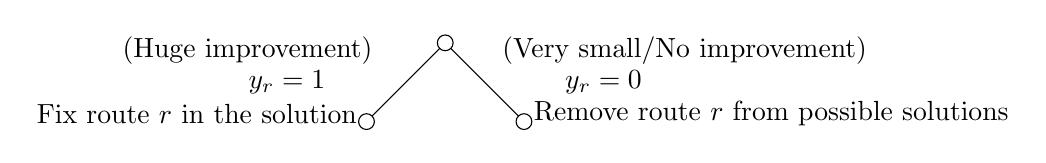
\begin{tikzpicture}[scale=0.2]
                    \draw (0, 5) circle [radius=0.5];
                    \draw (-5, 0) circle [radius=0.5];
                    \draw (5, 0) circle [radius=0.5];
                    \draw (0.353, 4.647) -- (4.647, 0.353);
                    \draw (-0.353, 4.647) -- (-4.647, 0.353);
                    \node [left] at (-7, 2.5) {$y_r = 1$};
                    \node [left] at (-5, 0.5) { Fix route $r$ in the solution};
                    \node [left] at (-4, 4.5) { (Huge improvement) };
                    \node [right] at (7, 2.5) {$y_r = 0$};
                    \node [right] at (5, 0.5) { Remove route $r$ from possible solutions};
                    \node [right] at (3, 4.5) { (Very small/No improvement) };
                \end{tikzpicture}
            \end{figure}

            The right sub-tree will continue to be searched very inefficiently, due to the unbalance of the tree. The good news is, there are possible improvements to this issue by applying different branching strategies. One of them is the Ryan-Foster Branching Rule, which is designed for the Set Covering Problem. For any fractional solution, there are at least two elements $(i,j)$ so that $i$ and $j$ are both partially covered by the same set $S$, but there is another set $T$ that only covers $i$
            \begin{figure}[h!]
                \centering
                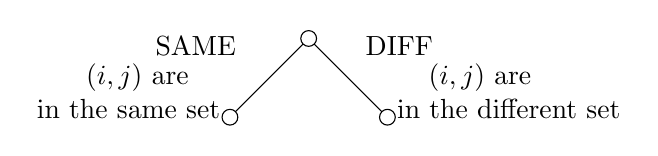
\begin{tikzpicture}[scale=0.2]
                    \draw (0, 5) circle [radius=0.5];
                    \draw (-5, 0) circle [radius=0.5];
                    \draw (5, 0) circle [radius=0.5];
                    \draw (0.353, 4.647) -- (4.647, 0.353);
                    \draw (-0.353, 4.647) -- (-4.647, 0.353);
                    \node [left] at (-7, 2.5) {$(i,j)$ are};
                    \node [left] at (-5, 0.5) { in the same set};
                    \node [left] at (-4, 4.5) {SAME};
                    \node [right] at (7, 2.5) {$(i,j)$ are};
                    \node [right] at (5, 0.5) { in the different set};
                    \node [right] at (3, 4.5) {DIFF};
                \end{tikzpicture}
            \end{figure}

            For the search go through the SAME branch, the following constraint will be added into the follow-up subproblems.

            \begin{equation*}
                \sum_{l: (i, l) \in E} w_{il} = \sum_{l: (j, l \in E)} w_{jl}
            \end{equation*}

            For the DIFF branch, the corresponded constraints will be

            \begin{equation*}
                \sum_{l: (i, l) \in E} w_{il} + \sum_{l: (j, l \in E)} w_{jl} \le 1
            \end{equation*}

            Second, there is a terrible symmetric issue/degeneracy issue in the subproblem - the subproblem will produce duplicate routes. One of the another solutions is for every route r in $y_r = 0$ branches, add the following constraints

            \begin{equation*}
                \sum_{(i, j) \in E, w_{ij}^r = 0, \forall r \in R^\prime} w_{ij} + \sum_{(i, j) \in E, w_{ij}^r = 1, \forall r \in R'} (1 - w_{ij}) \ge 1
            \end{equation*}

            The idea is to use the edges that have not yet been used more, and use the edges that have appeared in other edges less. (But it will still be bad...)
        
    \chapter{Benders Decomposition}
        \begin{center}
            \textit{``Learning from one's mistakes.''}
        \end{center}
        \section{Benders Decomposition}
            Benders Decomposition is usually applied for those problems that are easy to solve after fixing some of the variables. The general idea is to divide the problem into a master problem containing all complicated variables and subproblems containing simple variables. For example, given an MILP model as follows
            \begin{align*}
                \text{(MILP)} \quad \min \quad & f^\top y + c^\top x \\
                \text{s.t.} \quad & A y \ge b \\
                & By + Dx \ge d\\
                & x \ge 0\\
                & \mathbf{y} \in \mathbb{Y} \subseteq \mathbb{Z}_+
            \end{align*}

            In the formulation, decision variables $x$ are separable, thus, for a given $\bar{y} \in \mathbb{Y}$, a subproblem is defined a follows
            \begin{align*}
                \text{(Sub)} \quad \min \quad & f^\top \bar{y} + c^\top x\\
                \text{s.t.} \quad & B \bar{y} + Dx \ge d\\
                & x \ge 0
            \end{align*}

            In which $f^\top \bar{y}$ is a constant for given $\bar{y}$, rewrite (Sub) as follows

            \begin{align*}
                \text{(Sub)} \quad \eta(\bar{y}) = \min_x \{c^\top x | D x \ge d - B \bar{y}, x \ge 0\}
            \end{align*}

            Notice that $\bar{y}$ remains in the constraints of (Sub), every time when a new $\bar{y}$ is given, the feasible region changes, which makes it difficult to keep track of the model. To facilitate our analysis, we take the dual of (Sub), which maintains the same feasible region every time when a new $\bar{y}$ is given. The dual of the subproblem is defined as follows

            \begin{align*}
                \text{(Dual-Sub)} \quad \eta(\bar{y}) = \max_{\pi} \{\pi^\top (d - B\bar{y})| \pi^\top D \le c, \pi \ge 0\}
            \end{align*}

            Then, the equivalent formulation of the original problem is
            \begin{align*}
                \text{(Master)} \quad \min \quad & f^\top y + \eta\\
                & Ay \ge b\\
                & \eta \ge \max_\pi \{\pi^\top (d - By) | \pi^\top D \le c, \pi \ge 0\}\\
                & \mathbf{y} \in \mathbb{Y} \subseteq \mathbb{Z}_+
            \end{align*}

            Apply the Minkowski-Weyl Theorem to the (Dual-Sub), the feasible region $\{\pi|\pi^\top D \le c, \pi \ge 0\}$ can be represented by a set of extreme points (e.p.) and a set of extreme directions (e.d.). Thus, let

            \begin{itemize}
                \item $\pi_e \in V$ be the set of all extreme points, and 
                \item $\pi_d \in D$ be the set of all extreme directions
            \end{itemize}

            The original problem can be further rewritten as follows
            \begin{align*}
                \text{(Master)} \quad \min \quad & f^\top y + \eta\\
                & Ay \ge b\\
                & \eta \ge \pi_e^\top (d - By), \quad \forall \pi_e \in V\\
                & 0 \ge \pi_d^\top (d - By), \quad \forall \pi_d \in D\\
                & \eta \ge 0\\
                & \mathbf{y} \in \mathbb{Y} \subseteq \mathbb{Z}_+
            \end{align*}

            In which, $\eta \ge \pi_e^\top (d - By)$ are referred as optimality cuts, and $0 \ge \pi_d^\top (d - By)$ are referred as feasibility cuts. However, the set $V$ and $D$ are exponentially large, it is intractable if we have all feasibility cuts and optimality cuts added into the model. To reduce the computational burden, a Branch-and-Cut scheme algorithm framework is more widely implemented by researchers.

            Define the initial restricted master problem which only contains the integer variables $\mathbf{y}$ as follows

            \begin{align*}
                \text{(RMP)} \quad \min \quad &f^\top y + \eta\\
                & Ay \ge b \\
                & \eta \ge 0 \\
                & \mathbf{y} \in \mathbb{Y} \subseteq \mathbb{Z}_+
            \end{align*}

            Each iteration, an optimized $\bar{y}$ for the (RMP) will be given to the subproblem, which will create a (or multiple) optimality cut(s) or feasibility cut(s). Those cuts will be added into the model in a lazy manner. Each time when an optimality cut is found and added, the lower bound of the master problem will be lifted, otherwise, if a feasibility cut is found and added, the upper bound will be updated. The iteration terminates when the lower bound meet with the upper bound within an acceptable error.

        \section{A Uncapacitated Facilities Location Problem}
            \subsection{Formulation}
                Consider the following facility location problem, where $m$ is the number of potential facilities, $n$ is the number of customers, and $\mathbb{Y}$ is the set of feasible plans of facility location plans, where $\mathbf{y} \in \mathbb{Y} \subseteq \{0, 1\}^m$. $c_{ij}$ is the cost for customer $i$ to be assigned to facility $j$, $d_j$ is the cost for opening facility $j$. The formulation is as following
                
                \begin{table}[!htp]
                    \centering
                    \caption{Sets and Parameters}
                    \begin{tabular}{c|p{8cm}}
                        \hline
                        \textbf{Notations} & \textbf{Description} \\
                        \hline
                        $m$ & Number of potential facilities\\
                        $n$ & Number of customers\\
                        $F = \{1, 2, \ldots, m\}$ & Set of potential facilities \\
                        $C = \{1, 2, \ldots, n\}$ & Set of customers\\
                        $d_j$ & The cost of constructing facility $j$, where $j \in $.\\
                        $c_{ij}$& The cost for customer $i$ to receive service from facility $j$, where $i \in C$ and $j \in F$.\\
                        \hline
                    \end{tabular}
                \end{table}

                \begin{table}[!htp]
                    \centering
                    \caption{Decision variables}
                    \begin{tabular}{c|p{8cm}}
                        \hline
                        \textbf{Notations} & \textbf{Description}\\
                        \hline
                        $y_j$ & Binary variables, takes 1 if facility $j$ is decided to be constructed, where $j \in F$.\\
                        $x_{ij}$ & Continuous variables, the percentage of demand for customer $i$ to be fulfilled by facilities $j$, where $i \in C$ and $j \in F$.\\
                        \hline
                    \end{tabular}
                \end{table}

                \begin{align}
                    \text{(FLP)} \quad \min \quad & \sum_{i = 1}^n \sum_{j = 1}^m c_{ij} x_{ij} + \sum_{j = 1}^m d_j y_j \nonumber\\
                    \text{s.t.} \quad &\sum_{j = 1}^m x_{ij} \ge 1, \quad \forall i \in C \label{cons:demand}\\
                        &x_{ij} \le y_j, \quad \forall i \in C, j \in F \label{cons:open}\\
                        &x_{ij} \ge 0, \quad \forall i \in C, j \in F \label{cons:nonnegX}\\
                        &y_{j} \in \{0, 1\}, \quad \forall j \in F \label{cons:nonnegY}
                \end{align}

                In the formulation (FLP), 
                \begin{itemize}
                    \item Constraints (\ref{cons:demand}) indicate that for each customer $i$, its request needs to be fulfilled.
                    \item Constraints (\ref{cons:open}) indicate that a facility $j$ can only be able to serve customer $i$ if the facility is opened.
                    \item Constraints (\ref{cons:nonnegX}) is the nonnegative constraints for $\mathbf{x}$.
                    \item Constraints (\ref{cons:nonnegY}) defines $\mathbf{y}$ as binary variables.
                \end{itemize}

            \subsection{Solution Approach}
                If $y$ are fixed, i.e., $y = \bar{y} \in \mathbb{Y}$, the rest of the formulation will become an LP model with $x_{ij}$ as the nonnegative decision variables. 

                \begin{align*}
                    (\text{Sub}) \quad \min \quad & \sum_{i = 1}^n \sum_{j = 1}^m c_{ij} x_{ij} + \sum_{j = 1}^m d_j \bar{y_j}\\
                    \text{s.t.} \quad &\sum_{j = 1}^m x_{ij} \ge 1, \quad \forall i \in C\\
                        &x_{ij} \le \bar{y_j}, \quad \forall i \in C, j \in F\\
                        &x_{ij} \ge 0, \quad \forall i \in C, j \in F
                \end{align*}

                If we take the dual of this new LP, we get
                \begin{align*}
                    \text{(Dual-Sub)} \quad \max \quad & \sum_{i = 1}^n (\lambda_i - \sum_{j = 1}^m \bar{y}_j \pi_{ij}) + \sum_{j = 1}^m d_j \bar{y}_j \\
                    \text{s.t.} \quad & \lambda_i - \pi_{ij} \le c_{ij} \quad \forall i \in C, j \in F\\
                    & \lambda_i \ge 0\quad \forall i \in C\\
                    & \pi_{ij} \ge 0 \quad \forall i \in C, j \in F
                \end{align*}

                Now get rid of the constant in the objective function of (Sub) and (Dual-Sub), which is $\sum_{j = 1}^m d_j \bar{\mathbf{y}}$, we can then define

                \begin{align*}
                    \eta(\bar{\mathbf{y}}) &= \min_\mathbf{x} \{\sum_{i = 1}^n \sum_{j = 1}^m c_{ij} x_{ij} | \sum_{j = 1}^m x_{ij} \ge 1, x_{ij} \le \bar{y_j}, x_{ij} \ge 0, i \in C, j \in F\}\\
                    &= \max_\mathbf{\pi} \{\sum_{i=1}^n (\lambda_i - \sum_{j = 1}^m \bar{y_j} \pi_{ij})|\lambda_i - \pi_{ij} \le c_{ij}, \lambda_i \ge 0, \pi_{ij} \ge 0 i \in C, j \in F\}
                \end{align*}

                The (FLP) model can be equivalently rewritten as follows

                \begin{align*}
                    \text{(FLP)} \quad & = \min_{\bar{y} \in \mathbb{Y}}\{\sum_{j = 1}^m d_j \bar{y}_j + \eta(\bar{\mathbf{y}})\}\\
                    & = \min_{\bar{y} \in \mathbb{Y}} \{\sum_{j = 1}^m d_j \bar{y}_j + \max_\mathbf{\pi} \{\sum_{i=1}^n (\lambda_i - \sum_{j = 1}^m \bar{y_j} \pi_{ij})|\lambda_i - \pi_{ij} \le c_{ij}, \lambda_i \ge 0, \pi_{ij} \ge 0 i \in C, j \in F\}\}
                \end{align*}

                Notice that for index $i$, the customer, there is no constraint among them, which is logically to be true since in reality customers are not related to each other. 

                \begin{alignat*}{5}
                    \text{(Dual-Sub)} \quad v(\hat{\mathbf{y}}) = \max \quad & (\lambda_1 - \sum_{j = 1}^m \hat{y}_j \pi_{1j}) + &&(\lambda_2 - \sum_{j = 1}^m \hat{y}_j \pi_{2j}) + \ldots + &&(\lambda_n - \sum_{j = 1}^m \hat{y}_j \pi_{nj}) + && \sum_{j = 1}^m d_j \hat{y}_j \\
                    \text{s.t.} \quad                & \lambda_1 - \pi_{1j} \le c_{1j}                   &&                                                           &&                                                  && \quad \forall j \in \{1, 2, \ldots, m\}\\
                                                     &                                                   && \lambda_2 - \pi_{2j} \le c_{2j}                           &&                                                  && \quad \forall j \in \{1, 2, \ldots, m\}\\
                                                     & \cdots\\
                                                     &                                                   &&                                                           && \lambda_n - \pi_{nj} \le c_{nj}                  && \quad \forall j \in \{1, 2, \ldots, m\}\\
                                                     & \lambda_1 \ge 0                                   &&                                                           &&                                                  && \\
                                                     &                                                   && \lambda_i \ge 0                                           &&                                                  && \\
                                                     & \cdots\\
                                                     &                                                   &&                                                           && \lambda_n \ge 0                                  && \\
                                                     & \pi_{1j} \ge 0                                    &&                                                           &&                                                  && \quad j \in \{1, 2, \ldots, m\}\\
                                                     &                                                   && \pi_{2j} \ge 0                                            &&                                                  && \quad j \in \{1, 2, \ldots, m\}\\
                                                     & \cdots\\
                                                     &                                                   &&                                                           && \pi_{nj} \ge 0                                   && \quad j \in \{1, 2, \ldots, m\}\\
                \end{alignat*}

                Therefore, the due of subproblem can be further decomposed by $i$, for each $i$,

                \begin{align*}
                    \text{(Dual-Sub-$i$)} \quad \eta_i(\bar{\mathbf{y}}) = \max \quad & \lambda_i - \sum_{j = 1}^m \bar{y}_j \pi_{ij}\\
                    \text{s.t.} \quad & \lambda_i - \pi_{ij} \le c_{ij}, \quad \forall j \in F\\
                    & \lambda_i \ge 0, \quad \forall i \in C\\
                    & \pi_{ij} \ge 0, \quad \forall i \in C, j \in F
                \end{align*}

                The (Dual-Sub-$i$) can easily be solved as following
                \begin{align*}
                    &\bar{\lambda_i} = \min \{c_{ij}, j \in \mathbf{O}\}\\
                    &\begin{cases}
                        \bar{\pi_{ij}} = 0, \quad j \in \mathbf{O}\\
                        \bar{\pi_{ij}} = \max \{0, \bar{\lambda_i} - c_{ij}\}, \quad j \in \mathbf{C}
                    \end{cases}
                \end{align*}

                In which $\mathbf{O}$ is the set of indices $j$ where $\bar{y}_j = 1$ and $\mathbf{C}$ is the set of indices $j$ where $\bar{y}_j = 0$. The optimal value of dual variables can be interpreted in terms of facilities location problem. $\bar{\lambda_i}$ is the cost of serving customer $i$ when $y = \bar{y}$ and $\bar{\pi_{ij}}$ is the reduction in the cost of serving customer $i$ when facility $j$ is opened and $y_i = \bar{y_i}$.

                After solving the (Dual-Sub-$i$), we can find the objective function value as well as the dual variable values for (Dual-Sub). 

                The restricted master problem initialized with no additional constraints, as follows

                \begin{align*}
                    \text{(RMP)} \quad \min \quad & \sum_{j = 1}^m d_j y_j\\
                    \text{s.t.} \quad & \mathbf{y} \in \mathbb{Y}
                \end{align*}

                There is only one case where the (Dual-Sub) problem will be unbounded, which would be when $\bar{\mathbf{y}} = \mathbf{0}$. In that case, a feasibility cut will be added into the master problem, as follows
                \begin{equation}
                    0 \ge \sum_{i=1}^n (\bar{\lambda_i} - \sum_{j = 1}^m y_j \bar{\pi_{ij}})
                \end{equation}
                For other cases, as long as there is at least one facility opened, the Subproblem is always feasible, therefore, a feasibility cut will be added into the master problem, as follows
                \begin{equation*}
                    \eta \ge \sum_{i=1}^n (\bar{\lambda_i} - \sum_{j = 1}^m y_j \bar{\pi_{ij}})
                \end{equation*}

                The iteration continues until no more cut can be added into the master problem and we derive the optimal solutions.

        \section{Pareto-optimality cut}
            \subsection{Choosing procedure}
                \begin{definition}[dominance, pareto-optimal]
                    We say cut
                    \begin{equation}
                        z \ge hy + u^1(b - Dy) \succ z \ge hy + u^2(b - Dy)
                    \end{equation}
                    if
                    \begin{equation}
                        hy + u^1(b - Dy) \ge hy + u^2(b - Dy), \quad \forall y    
                    \end{equation}
                    with at least one strict inequality. Further, we call a cut \textbf{pareto optimal} if it is not dominated by any other cut.
                \end{definition}

                Notice that a Benders cut is determined by the vector $u$, so we want to find which of the produced multiple solutions to the subproblem are not dominated by others (i.e. which vectors produce pareto optimal cuts).

                Define a \textbf{core point} of $\mathbb{Y}$, $y^0 \in ri(\mathbb{Y}^c)$, which can be any point of the relative interior of convex hull of $\mathbb{Y}$.

                Assume that we have $\hat{y}$, the current solution to the master problem, and $v(\hat{y})$ is the optimal value of the subproblem. To find a pareto optimal cut among the multiple solutions $u$ of the dual of the subproblem $f(\hat{y})$, we solve the following linear program:

                \begin{align}
                    \max \quad & h^Ty^0 + u(b - Dy^0)\\
                    \text{s.t.} \quad & u(b - D\hat{y}) = v(\hat{y}) - h^T\hat{y} \label{cons:pareto1}\\
                    &uA \le c^T \label{cons:pareto2}
                \end{align}

                Constraints (\ref{cons:pareto1}) and (\ref{cons:pareto2}) ensure that we are searching only through alternative optimal solutions for the current subproblem. 

                Note that $y^0$ can be any arbitrary core point of $\mathbb{Y}$. In other words, choosing different core point and solving that problem we obtain different pareto optimal cut, among which we cannot tell which one is better.

                Let us see why is that true. Suppose that $y^0$ is a core point of $\mathbb{Y}$ and $U(\hat{y})$ is the set of optimal solutions to the subproblem:

                \begin{equation}
                    \max\{h^T\hat{y} + u(b - D\hat{y})\} \label{cons:sub}
                \end{equation}

                Let $u^0$ solve the problem:

                \begin{equation}
                    \max\{h^Ty^0 + u(b - Dy^0)\} \label{cons:sub0}
                \end{equation}  

                Now we can prove by contradiction that $u^0$ is not dominated by any other cut from $U(\hat{y})$. Suppose there exists $\bar{u}$, that dominates $u^0$:

                \begin{equation}
                    h^Ty + \bar{u}(b - Dy) \ge h^Ty + u^0(b - Dy)\ \ \forall y \in \mathbb{Y} \label{cons:dom}
                \end{equation}

                taking any point $w$ of the convex hull of $\mathbb{Y}^c$ (which can be represented as a convex combination of a finite number of points from $\mathbb{Y}$) we have:

                \begin{equation}
                    h^Tw + \bar{u}(b - Dw) \ge h^Tw + u^0(b - Dw)\ \ \forall w \in \mathbb{Y}^c
                \end{equation}

                note that with $y=\hat{y}$ in \ref{cons:dom}, $\bar{u}$ must be an optimal solution to \ref{cons:sub}. But then from \ref{cons:dom} and (\ref{cons:sub0}) we have:

                \begin{equation}
                    h^Ty + \bar{u}(b - Dy) = h^Ty + u^0(b - Dy)\ \ \forall y \in \mathbb{Y}
                \end{equation}

                and since $\bar{u}$ dominated $u^0$, there exists at least one $\bar{y}$ such that:

                \begin{equation}
                    h^T\bar{y} + \bar{u}(b - D\bar{y}) > h^T\bar{y} + u^0(b - D\bar{y})
                \end{equation}

            \subsection{Pareto Optimal Cuts for Facility Location Problem}
                Consider the previous facility location problem. If $y$ are fixed, i.e., $y = \hat{y} \in \mathbb{Y}$, the rest of the formulation will become a LP model with $x_{ij}$ as the nonnegative decision variables which can further be separated as a set of subproblems for each $i$, 
                \begin{alignat*}{2}
                    \text{(Dual-Sub-$i$)} \quad \max \quad & \lambda_i - \sum_{j = i}^m \hat{y}_j \pi_{ij}\\
                    \text{s.t.} \quad & \lambda_i - \pi_{ij} \le c_{ij}                  && \quad \forall j \in \{1, 2, \ldots, m\}\\
                                      & \lambda_i \ge 0                                  && \\
                                      & \pi_{ij} \ge 0                                   && \quad j \in \{1, 2, \ldots, m\}\\
                \end{alignat*}

                and each subproblem can be solved as following
                \begin{alignat*}{2}
                    &\hat{\lambda}_i = \min \{c_{ij}, j \in \mathbf{O}\} \\
                    &\hat{\pi}_{ij} = 0 &&\quad \text{ if } j \in \mathbf{O} \\
                    &\hat{\pi}_{ij} = \max\{0, \hat{\lambda}_i - c_{ij}\} &&\quad \text{ if } j \in \mathbf{C} \\
                \end{alignat*}

                then, the optimal objective function for the $i$th separated subproblem is $v_i(\mathbf{\hat{y}}) = \hat{\lambda}_i$. From our previous discussion, for each $i$, we can solve the following problem (Pareto-Sub-$i$) to get (part of) the Pareto-optimal cut $\mathbf{u}_{i} = (\lambda_i, \pi_{i1}, \pi_{i2}, \cdots, \pi_{im})$. (The Pareto-optimal cut is $\mathbf{u} = (\mathbf{u}_1, \mathbf{u}_2, \cdots, \mathbf{u}_n)$)

                \begin{alignat*}{2}
                    \text{(Pareto-Sub-$i$)} \quad \max \quad & \lambda_i - \sum_{j = i}^m y^0_j \pi_{ij}\\
                    \text{s.t.} \quad & \lambda_i - \sum_{j = i}^m \hat{y}_j \pi_{ij} = \hat{\lambda}_i\\
                                      & \lambda_i - \pi_{ij} \le c_{ij}                  && \quad \forall j \in \{1, 2, \ldots, m\}\\
                                      & \lambda_i \ge 0                                  && \\
                                      & \pi_{ij} \ge 0                                   && \quad j \in \{1, 2, \ldots, m\}\\
                \end{alignat*}

                where, as mentioned, $\mathbf{y}^0 \in ri(\mathbb{Y}^c)$. By observation, this problem can be solved as following. First, replace the objective function with the first equality constraint, then the formulation can be rewritten as

                \begin{alignat*}{2}
                    \text{(Pareto-Sub-$i$)} \quad \max \quad & \hat{\lambda}_i + \sum_{j = i}^m (\hat{y}_j - y_j^0) \pi_{ij}\\
                    \text{s.t.} \quad & \lambda_i - \pi_{ij} \le c_{ij}                  && \quad \forall j \in \{1, 2, \ldots, m\}\\
                                      & \lambda_i \ge 0                                  && \\
                                      & \pi_{ij} \ge 0                                   && \quad j \in \{1, 2, \ldots, m\}\\
                \end{alignat*}

                For those $j \in \mathbf{O}$, $\hat{y}_j = 1$, $\hat{y}_j - y_j^0 > 0$, for those $\pi_{ij}$ we want to maximize them, however, we have $\lambda_i - \hat{\lambda}_i = \sum_{j \in \mathbf{O}} \pi_{ij}$, i.e., summation of all such $\pi_{ij}$ is constrained, to maximize the objective function, we can choose the one where $\hat{y}_j - y_j^0$ is the most.

                For those $j \in \mathbf{C}$, $\hat{y}_j = 0$, $\hat{y}_j - y_j^0 < 0$, for those $\pi_{ij}$ we want to minimize them, therefore $\pi_{ij} = \max \{0, \lambda_i - c_{ij}\}$.

                Therefore, the objective function value will be a function of $\lambda_i$, or $f(\lambda_i)$ as 
                \begin{equation}
                    f(\lambda_i) = \hat{\lambda}_i + \max_j \{\hat{y}_j - y_j^0\} (\lambda_i - \hat{\lambda}_i) + \sum_{j \in \mathbf{C}} (\hat{y}_j - y_j^0)\max\{0, \lambda_i - c_{ij}\}
                \end{equation}

                This becomes a piece-wise linear function for $\lambda_i$, we can find the optimal value of $\lambda_i$ easily, and once it is found, $\pi_{ij}$ can be derived by $\max\{0, \lambda_i - c_{ij}\}$, therefore for a given $i$ we can get $\mathbf{u}_{i} = (\lambda_i, \pi_{i1}, \pi_{i2}, \cdots, \pi_{im})$. Repeat this for $n$ times, we can get the Pareto-optimal cut $\mathbf{u}$.

    \chapter{Heuristic and Metaheuristic Methods}
        \begin{center}
            \textit{``Puzzle.''}
        \end{center}

        \section{Heuristic-Search Procedures}

            The word ``heuristic'' stands for ``I found it'' in Greek. The heuristic algorithm are the procedures that we use some information available about the problem to
            \begin{itemize}
                \item reduce the search space
                \item or to speed up the search
                \item but not guarantee to find the optimum.
            \end{itemize}

            though there are some shortcomings about heuristic, still, we use heuristic because
            \begin{itemize}
                \item we need to avoid combinatorial explosion, because we need the solution FAST.
                \item we don't need the ``optimal'' solution, good approximation will be sufficient.
                \item The approximations may not be very good in the worst case, but in reality worst cases occur very rarely.
                \item Trying to understand why a heuristic works/does not work leads to a better understanding of the problem.
            \end{itemize}

            \subsection{Hill-Climbing: An Irrevocable Strategy}
                Hill-climbing is a local search algorithm used for optimization problems. It starts with an initial solution and iteratively makes small improvements by selecting a neighboring solution that improves the objective function. The process continues until no better neighboring solutions can be found, often resulting in a local optimum. It is simple and efficient but can get stuck in suboptimal solutions due to its greedy nature.

                The generic algorithm is as follows

                \begin{algorithm}[!htp]
                    \centering
                    \caption{Hill-climbing}
                    \begin{algorithmic}[1]
                        \State $S \gets$ an initial solution
                        \While {not \texttt{stopFlag}}
                            \State $R \gets$ \texttt{Neighbor(S.clone())}
                            \If {\texttt{OFV($R$)} is better than \texttt{OFV($S$)}}
                                \State $S \gets R$
                            \EndIf
                        \EndWhile
                        \State \Return $S$
                    \end{algorithmic}
                \end{algorithm}

                We can make this algorithm a little more aggressive: create $n$ neighbors to a candidate solution all at one time, and then possibly adopt the best one. This modified algorithm is called Steepest Ascent Hill-Climbing , because by sampling all around the original candidate solution and then picking the best, we’re essentially sampling the gradient and marching straight up it.

                The generic algorithm is as follows

                \begin{algorithm}[!htp]
                    \centering
                    \caption{Steep Ascent Hill-climbing}
                    \begin{algorithmic}[1]
                        \State $n \gets$ number of neighbors
                        \State $S \gets$ an initial solution
                        \While {not \texttt{stopFlag}}
                            \State $R \gets$ \texttt{Neighbor(S.clone())}
                            \For {$n - 1$ times}
                                \State $W \gets$ \texttt{Neighbor(S.clone())}
                                \If {\texttt{OFV($W$)} is better than \texttt{OFV($R$)}}
                                    \State $R \gets W$
                                \EndIf
                            \EndFor
                            \If {\texttt{OFV($R$)} is better than \texttt{OFV($S$)}}
                                \State $S \gets R$
                            \EndIf
                        \EndWhile
                        \State \Return $S$
                    \end{algorithmic}
                \end{algorithm}

                There are several weakness of the Hill-climbing algorithm:

                \begin{itemize}
                    \item They usually terminate at solutions that are only locally optimal.
                    \item There is no information as to the amount by which the discovered local optimum deviates from the global optimum, or perhaps even other local optima.
                    \item The optimum that's obtained depends on the initial configuration.
                    \item In general, it is not possible to provide an upper bound for the computation time.
                \end{itemize}

            \subsection{Uninformed Search}
                Uninformed search, also known as blind search, refers to a class of search algorithms that do not use any domain-specific knowledge or heuristic information to guide the search process. These algorithms explore the search space systematically without any additional information about the goal or the structure of the problem beyond the problem definition itself.

                \subsubsection{Depth-First and Backtracking: LIFO Search Strategies}

                    Depth-First Search (DFS) starts at a selected node (often the root in trees or any node in graphs) and explores as far as possible along each branch before backtracking. 

                    DFS uses a stack (either explicitly or through recursion) to keep track of nodes to visit. It is useful for tasks like solving mazes, topological sorting, and detecting cycles in graphs. However, it may not find the shortest path in unweighted graphs and can get stuck in infinite loops in graphs with cycles if not properly managed.

                \subsubsection{Breadth-First: A FIFO Search Strategy}

                    Breadth-First Search (BFS) explores all nodes at the present depth level before moving on to nodes at the next depth level.

                    BFS is useful for finding the shortest path in unweighted graphs, level-order traversal in trees, and solving puzzles like the shortest path in a maze. It ensures that all nodes at a particular depth are explored before moving deeper, making it effective for shortest-path problems. However, it can be memory-intensive due to the queue storing all nodes at the current depth level.

                \subsubsection{Iterative Deepening Search}
                
                    Iterative-Deepening Search combines BFS and DFS in an interesting way. IDS starts with a depth limit of 0 and increment it as long as it has not found a goal node. For every depth limit, IDS performs DFS up to the depth limit. This means that, if the current node is at the depth limit, IDS will not generate and add its successors to the frontier — essentially, IDS backtracks when it reaches the depth limit. Every time we increase the depth limit, IDS starts the depth-first search all over again.

                    IDS is an interesting hybrid of BFS and DFS. It is similar to DFS since it performs DFS for each depth limit. IDS is similar to BFS since it explores the search graph level by level by increasing the depth limit by one every time.

                    For space complexity, IDS performs DFS for every depth limit. Since IDS increases the depth limit by 1 each time, it will terminate at depth $d$, the depth of the shallowest goal node. The maximum length of the current path is $d$ and each node on the path has at most $b$ siblings.

                    Thus, the space complexity is $O(bd)$. This is linear in $d$, the depth of the shallowest goal node. The space complexity is similar to DFS.

                    In the worst case, IDS will visit all the nodes in the top $d$ levels. Thus, IDS’s time complexity is similar to that of BFS. The number of nodes up to depth $d$ is dominated by the number of nodes at depth $d$, which is $b^d$. Thus, the time complexity is $O(b^d)$. This is exponential in $d$, the depth of the shallowest goal node.

                    Some pros about IDS:

                    \begin{itemize}
                        \item Similar to DFS, IDS requires linear space only.
                        \item Similar to BFS, IDS is complete and is guaranteed to find the shallowest goal node.
                        \item IDS also has the same time complexity as BFS, although the exact number of nodes visited by IDS is larger than that of BFS.
                    \end{itemize}

            \subsection{Informed Search}
                Informed search, also known as heuristic search, refers to a class of search algorithms that use problem-specific knowledge or heuristic information to guide the search process. Unlike uninformed search algorithms, which explore the search space blindly, informed search algorithms leverage additional information (such as an estimate of the cost to reach the goal) to make more intelligent decisions about which paths to explore.

                For each node, we define the following notations for current node $n$.

                \begin{itemize}
                    \item $h(n)$ as the estimated cost from the current node $n$ to the destination.
                    \item $g(n)$ as the known (exact) actual cost from the start node to current node $n$
                    \item $f(n) = g(n) + h(n)$ is the heuristic knowledge. Think of $f(n)$ as an estimate of the cost of the cheapest path from the start state to a goal state through the current state $n$.
                \end{itemize}

                \subsubsection{A* search}
                    A* search explores the most promising next node, whereas depth first search goes as deep as possible in an arbitrary pattern and breadth first search explores all the nodes on one level before moving to the next. A* search uses a heuristic that provides a merit value for each node, whereas depth-first search and breadth-first search do not.

                    \begin{algorithm}
                        \centering
                        \caption{A* Search}
                        \begin{algorithmic}[1]
                        \State Initialize priority queue \texttt{Open} with $s$
                        \State Initialize set \texttt{Close} as empty
                        \State Initialize $f(s) = 0$
                        \While{$\texttt{Open} \neq \emptyset$}
                            \State $cur \gets$ node in \texttt{Open} with the lowest $f(n)$
                            \If{$cur == goal$}
                                \State \Return path found from $s$ to $cur$
                            \EndIf
                            \State $\texttt{Open} \gets \texttt{Open}\setminus \{cur\}$
                            \State $\texttt{Close} \gets \texttt{Close} \cup \{cur\}$
                            \For{each neighbor $n$ of $cur$}
                                \If{$n$ not in \texttt{Close}}
                                    \State $g^\prime(n) \gets g(cur) + cost(cur, n)$
                                    \If{$n$ not in \texttt{Open} or $g^\prime(n) < g(n)$}
                                        \State $g(n) \gets g^\prime(n)$
                                        \State $f(n) \gets g(n) + h(n)$
                                        \If{$n$ not in \texttt{Open}}
                                            \State Add $n$ to \texttt{Open}
                                        \EndIf
                                    \EndIf
                                \EndIf
                            \EndFor
                        \EndWhile
                        \end{algorithmic}
                    \end{algorithm}

                \subsubsection{Uniform Cost Search}
                    A special case of the A* search, where $h(n) = 0$, use the cost only. Technically this is not an informed search.

                \subsubsection{Best-first search}
                    Another special case of the A* search, where $g(n) = 0$, use the heuristic only.

        \section{Single-State Metaheuristic Methods}
            \subsection{Simulated Annealing}
                    Simulated Annealing is a probabilistic optimization technique inspired by the annealing process in metallurgy, where a material is heated and then slowly cooled to reduce defects. SA explores the solution space by accepting worse solutions with a certain probability, allowing it to escape local optima.

                    Simulated Annealing varies from Hill-Climbing in its decision of when to replace the original solution $S$ with a newly found neighborhood $R$. Specially, if $R$ is better than $S$, we always replace $S$ with $R$ as usual. But if $R$ is worse than $S$, we may still replace $S$ with $R$ with a certain probability $P(t, R, S)$:

                    \begin{equation}
                        P(t, R, S) = e^{\frac{\texttt{OFV(R)} - \texttt{OFV(S)}}{t}}, t > 0
                    \end{equation}

                    The generic algorithm for Simulated Annealing is as follows

                    \begin{algorithm}[!htp]
                        \centering
                        \caption{Simulated Annealing}
                        \begin{algorithmic}[1]
                            \State $t \gets$ initial temperature
                            \State $S \gets$ initial candidate solution
                            \State $Best \gets S$
                            \While {not \texttt{stopFlag}}
                                \State $R \gets$ \texttt{Neighbor(S.clone())}
                                \If {\texttt{OFV(R)} better than \texttt{OFV(S)}}
                                    \State $S \gets R$
                                \ElsIf {\texttt{Rnd()} $< e^{\frac{\texttt{OFV(R)} - \texttt{OFV(S)}}{t}}$}
                                    \State $S \gets R$
                                \EndIf
                                \State Decrease $t$
                                \If {\texttt{OFV(S)} better than \texttt{OFV(Best)}}
                                    \State $Best \gets S$
                                \EndIf
                            \EndWhile
                            \State \Return $Best$
                        \end{algorithmic}
                    \end{algorithm}

            \subsection{Tabu Search}
                    Tabu Search is a way of using memory in exchange of runtime. It keeps around a history of ``recently'' considered candidate solutions (known as a tabu list) and refuses to return to those candidates until they are sufficiently far in the past. Thus if we wander up a hill, we have no choice but to wander back down the other side because we are not permitted to stay at or return to the top of the hill. The key to Tabu Search is to maintain the tabu list with some maximum length. 

                    The generic algorithm for Tabu Search is as follows

                    \begin{algorithm}[!htp]
                        \centering
                        \caption{Tabu Search}
                        \begin{algorithmic}[1]
                            \State $l \gets$ desired maximum tabu list length
                            \State $n \gets$ number of new neighbor generate from current solution
                            \State $S \gets$ an initial solution
                            \State $Best \gets S$
                            \State $L \gets \{\}$ as a tabu list of length $l$
                            \State $L.enqueue(S)$
                            \While {not \texttt{stopFlag}}
                                \While {$L.length > l$}
                                    \State $L.pop()$
                                \EndWhile
                                \State $R \gets$ \texttt{Neighbor(S.clone())}
                                \For {$n$ times}
                                    \State $W \gets$ \texttt{Neighbor(S.clone())}
                                    \If {$W \notin L$ and \texttt{OFV($W$)} better than \texttt{OFV($R$)} or $R \in L$}
                                        \State $R \gets W$
                                    \EndIf
                                \EndFor
                                \If {$R \notin L$}
                                    \State $S \gets R$
                                    \State $L.enqueue(R)$
                                \EndIf
                                \If {\texttt{S} better than \texttt{Best}}
                                    \State $Best \gets S$
                                \EndIf
                            \EndWhile
                            \State \Return $Best$
                        \end{algorithmic}
                    \end{algorithm}

            \subsection{Iterated Local Search}
                    Iterated Local Search (ILS) tries to search through the space of local optima in a more intelligent fashion: it tries to stochastically hill-climb in the space of local optima. That is, ILS finds a local optimum, then looks for a ``nearby'' local optimum and possibly adopts that one instead, then finds a new ``nearby'' local optimum, and continue. The heuristic here is that you can often find a better local optima near to the current one, and walking from local optimum to local optimum in this way often outperforms just trying new locations entirely random.

                    There are two tricks in ILS, first, ILS does not pick a new restart location entirely at random, it maintains a ``home base'' local optimal and selects new restart locations that are near to the ``home base'' but not too close. We want the restart to be far away enough from current home base to wind up in a new local optimum, but not too far to be total random restart.

                    Second, when ILS discovers a new local optimum, it decides whether to retain the current ``home base'' local optimum, or to adopt the new local optimum as the ``home base''. There are two extremes on the spectrum, if we always accept the new local optimum no matter what, we are doing a random walk, if we always accept the local optimum when it is better than our current one, we are doing hill-climbing. ILS is something in-between those two extremes.

                    The generic algorithm for ILS is as follows
                    \begin{algorithm}[!htp]
                        \centering
                        \caption{Iterated Local Search with Random Restarts}
                        \begin{algorithmic}[1]
                            \State $T \gets$ possible time intervals
                            \State $S \gets$ an initial solution
                            \State Update ``home base'' $H \gets S$
                            \State $Best \gets S$
                            \While {not \texttt{stopFlag}}
                                \State $t \gets$ random time in the near future, sample from $T$
                                \While {not run out to time $t$}
                                    \State $R \gets$ \texttt{Neighbor(S.clone())}
                                    \If {\texttt{OFV($R$)} better than \texttt{OFV($S$)}}
                                        \State $S \gets R$
                                    \EndIf
                                    \If {\texttt{OFV($S$)} better than \texttt{OFV($Best$)}}
                                        \State $Best \gets S$
                                    \EndIf
                                    \State $H \gets$ New ``home base'' according to $S$
                                    \State $S \gets$ \texttt{Perturb($H$)}
                                \EndWhile
                            \EndWhile
                            \State \Return Best
                        \end{algorithmic}
                    \end{algorithm}

            \subsection{Greedy Randomized Adaptive Search Procedures}
                The Greedy Randomized Adaptive Search Procedures (GRASP) is a component-oriented method, designed for certain kinds of spaces consist of combinations of components drawn from a typically fixed set. It's the presence of this fixed set that we can take advantage of in a greedy, local fashion by maintaining historical ``quality'' values of individual components rather than complete solutions.

                GRASP is built on the notions of constructing and searching neighbors for feasible solutions, but it does not use any notion of component-level ``historical quality''. The overall algorithm is as follows: we create a feasible solution by constructing from among highest value (lowest cost) components and the do hill-climbing on the solution.

                \begin{algorithm}[!htp]
                    \centering
                    \caption{Greedy Randomized Adaptive Search Procedures (GRASP)}
                    \begin{algorithmic}[1]
                        \State $C \gets \{C_1, \cdots, C_n\}$ as a set of components
                        \State $p \gets$ percentage of components to include each iteration
                        \State $m \gets$ length of time to do hill-climbing
                        \State $Best \gets $\texttt{None}
                        \While {not \texttt{stopFlag}}
                            \State $S \gets \{\}$ as candidate solution
                            \While {$S$ is not a feasible solution}
                                \State $C^\prime \gets C_i \in C \setminus S$ which could be added to $S$ without being infeasible
                                \If {$C^\prime = \emptyset$}
                                    \State $S \gets \{\}$
                                \Else
                                    \State $C^{\prime\prime} \gets$ the $p\%$ highest value components in $C^\prime$
                                    \State $S \gets S \cup \{$component chosen uniformly at random from $C^{\prime\prime}\}$
                                \EndIf
                            \EndWhile
                            \For {$m$ times}
                                \State $R \gets$ \texttt{Neighbor(S.clone())}
                                \Comment $R$ need to remain feasible
                                \If {\texttt{OFV($R$)} better than \texttt{OFV($S$)}}
                                    \State $S \gets R$
                                \EndIf
                            \EndFor
                            \If {$B == $\texttt{None} or \texttt{OFV($S$)} better than \texttt{OFV($Best$)}}
                                \State $Best \gets S$
                            \EndIf
                        \EndWhile
                        \State \Return $Best$
                    \end{algorithmic}
                \end{algorithm}

        \section{Population-based Metaheuristic Methods}
            \subsection{Evolution Strategies}
                The family of evolution algorithms are based on a simple procedure for selecting individuals called truncation selection, and only use mutation as neighborhood searching operator. The simplest implementation is the $(\mu, \lambda)$ algorithm. We begin with a population of $\lambda$ number of randomly generated individuals. Each iteration we access the fitness of each individual and remove all but the $\mu$ fittest ones. Each of the $\mu$ fittest individuals get to produce descendants to repopulate the group until the number of individuals recover to $\lambda$ number.

                \begin{algorithm}[!htp]
                    \centering
                    \caption{The $(\mu, \lambda)$ Evolution Strategy}
                    \begin{algorithmic}[1]
                        \State $\mu \gets$ number of parents selected
                        \State $\lambda \gets$ number of children generated by the parents
                        \State $P \gets \{\}$
                        \While {$P.size < \lambda$}
                            \State $P \gets P \cup \{$new random individual$\}$
                        \EndWhile
                        \State $Best \gets$ the best individual among $P$
                        \While {not \texttt{stopFlag}}
                            \For {Each $P_i \in P$}
                                \If {\texttt{OFV(P$_i$)} better than \texttt{OFV(Best)}}
                                    \State $Best \gets P_i$
                                \EndIf
                            \EndFor
                            \State $Q \gets$ $\mu$ individuals in $P$ whose $OFV()$ are better
                            \State $P \gets \{\}$\Comment For $(\mu + \lambda)$, change it to $P \gets Q$
                            \For {Each $Q_i \in Q$}
                                \For {$\frac{\lambda}{\mu}$ times}
                                    \State $P \gets P \cup \{$ \texttt{Mutate(Q.clone())} $\}$
                                \EndFor
                            \EndFor
                        \EndWhile
                        \State \Return $Best$
                    \end{algorithmic}
                \end{algorithm}
                
                The $(\mu, \lambda)$ algorithm has three knobs with which we may adjust exploration versus exploitation.

                \begin{itemize}
                    \item The size of $\lambda$. This essentially controls the sample size for each population, and is basically the same thing as the $n$ variable in Steepest-Ascent Hill Climbing With Replacement. At the extreme, as $\lambda$ approaches $\infty$, the algorithm approaches exploration (random search).
                    \item The size of $\mu$. This controls how selective the algorithm is; low values of $\mu$ with respect to $\lambda$ push the algorithm more towards exploitative search as only the best individuals survive.
                    \item The degree to which Mutation is performed. If Mutate has a lot of noise, then new children fall far from the tree and are fairly random regardless of the selectivity of $\mu$
                \end{itemize}

            \subsection{Genetic Algorithm}
                The Genetic Algorithm is similar to the $(\mu, \lambda)$ Evolution Strategy in many respects: it iterates through fitness assessment, selection and breeding, and population reassembly. The primary difference is in how selection and breeding take place: whereas Evolution Strategies select all the parents and then create all the children, the Genetic Algorithm little-by-little selects a few parents and generates a few children until enough children have been created.To breed, we begin with an empty population of children. We then select two parents from the original population, copy them, cross them over with one another, and mutate the results. This forms two children, which we then add to the child population. We repeat this process until the child population is entirely filled.

                \begin{algorithm}[!htp]
                    \centering
                    \caption{Genetic Algorithm}
                    \begin{algorithmic}[1]
                        \State $p \gets$ size of population
                        \State $P \gets \{\}$
                        \While {$P.size < p$}
                            \State $P \gets P \cup \{$new random individual$\}$
                        \EndWhile
                        \State $Best \gets$ the best individual among $P$
                        \While {not \texttt{stopFlag}}
                            \For {Each $P_i \in P$}
                                \If {\texttt{OFV(P$_i$)} better than \texttt{OFV(Best)}}
                                    \State $Best \gets P_i$
                                \EndIf
                            \EndFor
                            \State $Q \gets \{\}$
                            \For {$p / 2$ times}
                                \State Select a Parent $P_a \gets$ \texttt{Select(P)}
                                \State Select another parent $P_b \gets$ \texttt{Select(P)}
                                \State Breed children $C_a, C_b \gets$ \texttt{Crossover(P$_a$, P$_b$)}
                                \State $Q \gets Q \cup \{C_a, C_b\}$
                            \EndFor
                            \State $P \gets Q$
                        \EndWhile
                        \State \Return $Best$
                    \end{algorithmic}
                \end{algorithm}

            \subsection{Particle Swarm Optimization}
                Particle Swarm Optimization (PSO) is a stochastic optimization technique somewhat similar to evolutionary algorithms but different in an important way. It’s modeled not after evolution per se, but after swarming and flocking behaviors in animals. Unlike other population-based methods, PSO does not resample populations to produce new ones: it has no selection of any kind. Instead, PSO maintains a single static population whose members are Tweaked in response to new discoveries about the space. The method is essentially a form of directed mutation.

                The key differential between the GA and PSO are threefold: 
                \begin{itemize}
                    \item first, in GA, each individual moves in discrete space, each represents a discrete solution, while in PSO, each particle moves in continue space, the location of each particle represents a continuum option.
                    \item second, in GA, individuals will be removed due to selection, but in PSO, the particles never die since there is no selection
                    \item third, GA improves the population mainly by crossover, however, PSO improves the population by mutation.
                \end{itemize} 

                \begin{algorithm}[!htp]
                    \centering
                    \caption{Particle Swarm Optimization}
                    \begin{algorithmic}[1]
                        \State $s \gets$ size of swarm
                        \State $\alpha \gets$ proportion of velocity to be retained
                        \State $\beta \gets$ proportion of personal best to be retained
                        \State $\delta \gets$ proportion of global best to be retained
                        \State $\epsilon \gets$ jump size of a particle
                        \State $P \gets \{\}$
                        \While {$P.size < s$}
                            \State $P \gets P \cup \{$new random individual $(\mathbf{x}, \mathbf{v})\}$
                        \EndWhile
                        \State $Best \gets$ the best individual among $P$
                        \While {not \texttt{stopFlag}}
                            \For {Each $P_i \in P$}
                                \If {\texttt{OFV(P$_i$)} better than \texttt{OFV(Best)}}
                                    \State $Best \gets P_i$
                                \EndIf
                            \EndFor
                            \For {$\mathbf{x_i} \in P$ with velocity $\mathbf{v_i}$}
                                \State $\mathbf{x^*} \gets$ location of previous best solution
                                \State $\mathbf{x^+_i} \gets$ location of $i$'s previous best location
                                \State Update speed $\mathbf{x_i} \gets \mathbf{x_i} + \epsilon (\alpha\mathbf{v_i} + \beta(\mathbf{x}^* - \mathbf{x_i}) + \delta(\mathbf{x^+}_i - \mathbf{x}_i))$
                            \EndFor
                        \EndWhile
                        \State \Return $Best$
                    \end{algorithmic}
                \end{algorithm}

            \subsection{Ant Colony Optimization}
                ACO is population-oriented. But there are two different kinds of ``populations'' in ACO. First, there is the set of components that make up a candidate solutions to the problem. In the Knapsack problem, this set would consist of all the blocks. In the TSP, it would consist of all the edges. The set of components never changes: but we will adjust the ``fitness'' (called the pheromone) of the various components in the population as time goes on.

                Each generation we build one or more candidate solutions, called ant trails in ACO parlance, by selecting components one by one based, in part, on their pheromones. This constitutes the second ``population'' in ACO: the collection of trails. Then we assess the fitness of each trail. For each trail, each of the components in that trail is then updated based on that fitness: a bit of the trail’s fitness is rolled into each component’s pheromone.

                \begin{algorithm}[!htp]
                    \centering
                    \caption{Ant Colony Optimization (ACO)}
                    \begin{algorithmic}[1]
                        \State $C \gets \{C_1, \cdots, C_n\}$ as a set of components
                        \State $p \gets$ size of population
                        \State $\mathbf{p} \gets (p_1, p_2, \cdots, p)$ as the pheromones of the components, initially 0
                        \State $Best \gets$ \texttt{None}
                        \While {not \texttt{stopFlag}}
                            \State $P \gets p$ trails built by iteratively selecting components based on pheromones and costs or values
                            \For {$P_i \in P$}
                                \State $P_i \gets$ \texttt{HillClimb($P_i$)}
                                \If {$B == $\texttt{None} or \texttt{OFV($S$)} better than \texttt{OFV($Best$)}}
                                    \State $Best \gets S$
                                \EndIf
                            \EndFor
                            \State Update $\mathbf{p}$ the pheromones for each $P_i \in P$
                        \EndWhile
                        \State \Return $Best$
                    \end{algorithmic}
                \end{algorithm}

        \section{Tuning the evolutionary algorithms}
            Almost every practical heuristic search algorithm is controlled by some set of parameters. E.g.,

            \begin{itemize}
                \item Genetic algorithm: population size, cross over rate, mutation rate, runtime limit, etc.
                \item Tabu search: tabu list length, tabu age, number of neighborhoods, runtime limit, etc.
                \item Simulated annealing: initial temperature, length staying at a temperature, accept rate, cooling rate, runtime limit, etc.
                \item $\cdots$
            \end{itemize}

            These parameters are applied to

            \begin{itemize}
                \item the representation
                \item the evaluation function
                \item the neighborhood searching operators
                \item the population size
                \item the stopping criteria
                \item $\cdots$
            \end{itemize}

            Since there are too many combinations of deciding the parameters, the trial-and-error method becomes very tedious and time-consuming, we need a theory to guide how to set some of the parameters of evolutionary algorithms.

            In general, there are two types of parameter settings:

            \begin{itemize}
                \item Parameter tuning: offline parameter search - before the GA is running
                \begin{itemize}
                    \item Parameter sweep (try everything)
                    \item Meta-GA ontop of GA
                    \item Racing strategy to find best parameters
                \end{itemize}
                \item Parameter control: online parameter search - during the GA is running
                \begin{itemize}
                    \item Deterministic genetic operators
                    \item Adaptive probabilities for mutation and crossover
                    \item Self-adaptive population size
                \end{itemize}
            \end{itemize}
            % \bibliography{literature}
\end{document}